\documentstyle[11pt,german,fleqn,psfig,DINA4]{artikel}
%\sloppy
\setlength{\parskip}{11pt}
\parindent=0pt
\pagestyle{headings}
\unitlength1cm
\mathindent1cm
%\includeonly{sa,sa6,lit}
\hyphenation{Sym-bol-ta-bel-le Sym-bol-ta-bel-len}
\renewcommand{\topfraction}{0.999}
\renewcommand{\bottomfraction}{0.999}
\renewcommand{\textfraction}{0.001}
\setcounter{topnumber}{2}
\setcounter{bottomnumber}{2}
\setcounter{totalnumber}{2}

\begin{document}

\tableofcontents

%\section{Einf"uhrung}
\label{einf}

%Neuronale Netze stellen eine Alternative zu "`klassischen"' symbolischen
%oder numerischen Verfahren dar, die f"ur geeignete Aufgabenstellungen
%einfachere und bessere Ergebnisse liefern kann.
%Einsatzbereiche sind z.B. die Mustererkennung oder das Verstehen und
%Verarbeiten von Bildern.
%Charakteristisch f"ur neuronale Netze ist, da"s die L"osung eines Problems
%nicht {\sl programmiert}, sondern anhand von Daten {\sl gelernt} wird.

%Jedes neuronale Netz besteht aus einer Menge von Neuronen bzw. Zellen,
%die untereinander durch ein gewichtetes Netzwerk verbunden sind.
%Jedes Neuron nimmt dabei zu jedem Zeitpunkt einen bestimmten 
%Aktivierungszustand an und besitzt einen Ausgabewert, der sich aus
%dem Aktivierungszustand durch Anwendung einer zum Neuron geh"orenden
%Ausgabefunktion berechnet. 

%Neuronen k"onnen in Eingabezellen, Ausgabezellen und "`versteckte"'
%Zellen eingeteilt werden.  
%Das neuronale Netz wird {\sl trainiert}, indem Eingabemuster 
%an die Eingabezellen
%angelegt werden (d.h. die Aktivierungen der Eingabezellen gesetzt werden)
%und in mehreren Schritten die Aktivierungen aller Zellen aus 
%den Ausgabewerten ihrer Vorg"anger sowie der 
%Gewichte der zugeh"origen Verbindungen neu berechnet werden.
%Anschlie"send werden die Werte der Ausgabezellen mit den gew"unschten
%Werten verglichen und die Gewichte der Verbindungen gem"a"s einer
%Lernregel in Abh"angigkeit von den beobachteten Abweichungen modifiziert.
%Das neuronale Netz {\sl lernt}.

Aufgabe der Studienarbeit war der Entwurf und die Implementierung eines
Programms, mit dem Eingabe- und Ausgabemuster f"ur neuronale Netze
transformiert und visualisiert werden k"onnen.
Als Eingabemuster ist hierbei ein Vektor zu verstehen, dessen Elemente
die Aktivierungen der Eingabezellen des neuronalen Netzes repr"asentieren.
Analog ist ein Ausgabemuster ein Vektor der Ausgabewerte der 
Ausgabezellen.
Trainings- bzw. Testdaten eines Netzes sind also
eine Menge von Eingabevektoren mit den zugeh"origen Ausgabevektoren.
Zur Spezifikation der Ausgabe werden zus"atzlich zu oder anstelle von den
Ausgabevektoren Klassen eingesetzt, die durch Nummern oder Klassensymbole
repr"asentiert werden.

Bevor Trainings- oder Testdaten in einem Simulator f"ur neuronale
Netze (wie z.B. KNet oder SNNS -- Stuttgarter Neuronale Netze Simulator --
der Universit"at Stuttgart) benutzt werden, ist es h"aufig w"unschenswert,
sich die Daten zun"achst graphisch oder textuell anzusehen und 
ggf.~einen oder mehrere Vorverarbeitungsschritte auf sie anzuwenden.
Desweiteren ben"otigen Simulatoren f"ur neuronale Netze zum Teil
sehr unterschiedliche Dateiformate f"ur die einzulesenden bzw.
zu schreibenden Trainingsvektoren.

Im Rahmen dieser Studienarbeit wurde das Programm "`Vistra"' entwickelt, das
\begin{itemize}
\item Trainingsdaten unterschiedlicher Formate lesen und schreiben
kann (Konvertierungsfunktion),
\item Trainingsdaten textuell und graphisch darstellen kann
(Visualisierungsfunktion),
\item Trainingsdaten transformieren und statistisch
auswerten kann (Manipulationsfunktion) sowie
\item um neue ASCII-Formate f"ur Trainingsvektor-Dateien erweitert werden 
kann mittels Vistra's Format-Beschreibungssprache FDL.
\end{itemize}
Durch die Konvertierungsfunktion ist Vistra vollkommen unabh"angig 
vom verwendeten Simulator f"ur neuronale Netze. 
Das Programm kann ganz allgemein zur Visualisierung und Manipulation von
Trainingsvektoren verwendet werden.

Auch eine Trennung von Trainings- und Testdaten wird unterst"utzt,
indem alle Transformationen, die auf einer Menge von Vektoren
ausgef"uhrt werden, in einer LOG-Datei festgehalten werden k"onnen.
Zu einem sp"ateren Zeitpunkt k"onnen die gleichen Transformationen 
dann mit einer anderen Menge von Trainingsvektoren wiederholt werden.
Zu diesem Zweck besitzt Vistra neben der interaktiven Benutzeroberfl"ache
auch noch einen Batch-Modus, in dem die in der LOG-Datei registrierten
Transformationen ausgef"uhrt werden k"onnen. 

Vistra wurde mit dem Gnu-C-Compiler (GCC) implementiert und verwendet
X-Windows (X11 Release 5) sowie das Athena Widget Set zur Realisierung
der graphischen Benutzer\-oberfl"ache. 
Vistra kann auf UNIX-Workstations der Fabrikate SUN und DEC compiliert
werden.

%\section[Funktionalit"at, Installation und Aufruf]{Funktionalit"at, 
Installation und Aufruf von Vistra}
\label{funk}

Dieses Kapitel gibt einen "Uberblick "uber die Funktionalit"at
von Vistra. 
Die Funktionen werden an dieser Stelle jedoch nur aufgelistet.
Eine detaillierte Bedienungsanleitung des Programms ist 
Gegenstand der n"achsten Kapitel.
Anschlie"send wird beschrieben, wie Vistra installiert wird und
wie die Syntax des Programmaufrufs mit seinen Optionen lautet.
 
\subsection{Funktionalit"at}
Die Funktionen von Vistra k"onnen in die drei Kategorien
{\sl Datei-Funktionen (Konvertierung), Transformationen} und
{\sl Visualisierungen} eingeteilt werden.

\subsubsection*{Datei-Funktionen (Konvertierung)}

Abbildung~\ref{flow} zeigt alle Arten von Dateien, die von Vistra
gelesen bzw.~geschrieben werden:

\begin{figure}[ht]
\hspace*{0.3cm}
\begin{picture}(14.4,6)
\put(0,4.8){\framebox(4,1.2){\parbox{4cm}
         {\begin{center} Trainingsvektor- \\ dateien \end{center}}}}
\put(0,3.2){\framebox(4,1.2){\parbox{4cm}
         {\begin{center} LOG-Dateien \end{center}}}}
\put(0,1.6){\framebox(4,1.2){\parbox{4cm}
         {\begin{center} Symboltabellen- \\ dateien \end{center}}}}
\put(0,0){\framebox(4,1.2){\parbox{4cm}
         {\begin{center} Formatbeschreibungs- \\ dateien \end{center}}}}
\put(5.2,2){\framebox(4,2){\parbox{4cm}
         {\begin{center} {\Large {\bf Vistra}} \end{center}}}}
\put(10.4,4){\framebox(4,1.2){\parbox{4cm}
         {\begin{center} Trainingsvektor- \\ dateien \end{center}}}}
\put(10.4,2.4){\framebox(4,1.2){\parbox{4cm}
         {\begin{center} LOG-Dateien \end{center}}}}
\put(10.4,0.8){\framebox(4,1.2){\parbox{4cm}
         {\begin{center} Symboltabellen- \\ dateien \end{center}}}}
\put(4,0.6){\vector(2,3){1.2}}
\put(4,2.2){\vector(2,1){1.2}}
\put(4,3.8){\vector(2,-1){1.2}}
\put(4,5.4){\vector(2,-3){1.2}}
\put(9.2,2.6){\vector(1,-1){1.2}}
\put(9.2,3){\vector(1,0){1.2}}
\put(9.2,3.4){\vector(1,1){1.2}} 
\end{picture}
\caption{\label{flow} Eingabe und Ausgabe von Vistra}
\end{figure}

Folgende Aktionen sind m"oglich:
\begin{itemize}

\item Trainingsvektor-Dateien unterschiedlicher Formate k"onnen eingelesen
und geschrieben werden. 
Zwei Formate stehen standardm"a"sig zur Verf"ugung:
\begin{itemize}
\item das N01-Format und
\item das LVQ-Format.
\end{itemize}
Beide Formate werden u.a. von KNet der Universit"at Stuttgart,
einem parallelen Simulator f"ur die selbstorganisierenden Karten
von Teuvo Kohonen (Kohonen Feature Maps), verwendet
(siehe \cite{bayer}). 
Das LVQ-Format ist ein ASCII-Format und stammt urspr"unglich
aus dem LVQ\_PAK, einem Public-Domain Paket, das "uber 
Internet von der Kohonen-Gruppe zur Verf"ugung gestellt 
wird\footnote{erh"altlich "uber die Internet-Adresse cochlea.hut.fi}.

Beim N01-Format handelt es sich um ein bin"ares Format. 
Die Vektoren liegen in maschinencodierter Form vor.
Bin"are Formate haben den Vorteil gegen"uber ASCII-Formaten, da"s sie
schneller eingelesen bzw.~geschrieben werden k"onnen, da 
zeitaufwendige Konvertierungen von Strings in Flie"skommazahlen 
vermieden werden.
Nachteilig ist, da"s sie maschinenabh"angig sind und vom Menschen
nicht gelesen werden k"onnen. 
Obwohl SUN- und DEC-Workstations unterschiedliche Codierungen f"ur
Zahlen verwenden, kann Vistra N01-Formate auf beiden Fabrikaten
lesen und schreiben.

Trainingsvektoren k"onnen in einem Format gelesen und in einem anderen
Format geschrieben werden.
Dadurch ist Vistra in der Lage, eine Vektordatei
von einem Format in ein anderes zu konvertieren.
N01- und LVQ-Format sind in Kapitel~\ref{formate} detailliert beschrieben.

\item Symboltabellen k"onnen eingelesen und geschrieben werden. 
Anstelle eines Ausgabevektors, wird einem Eingabevektor h"aufig nur
ein Symbol (ein String) zur Klassifikation der Ausgabe zugeordnet.
Eine Symboltabellen-Datei enth"alt dann eine Liste dieser Klassensymbole. 
Das genaue Aussehen von Symboltabellen-Dateien kann Kapitel~\ref{formate}
entnommen werden.

\item Neben dem LVQ-Format kann Vistra um weitere ASCII\--For\-mate 
f"ur Trainings\-vektor-Dateien erweitert werden.
Voraussetzung ist, da"s sich das Format durch Vistra's 
Formatbeschreibungssprache FDL ({\bf F}ormat {\bf D}escription 
{\bf L}anguage) 
hinreichend beschreiben l"a"st.
Ist dies der Fall, so kann Vistra ein solches Format sowohl lesen als
auch schreiben.
Zu diesem Zweck wurde ein Interpreter f"ur FDL entwickelt. 
FDL ist ausf"uhrlich in Kapitel~\ref{fdl} beschrieben.  

\item Vistra kann die auf den Trainingsvektoren durchgef"uhrten
Transformationen in einer LOG-Datei festhalten.
Dadurch wird es z.B.~m"oglich, mit Trainings- und Testvektoren, die zu
unterschiedlichen Zeitpunkten bzw. in separaten Dateien zur Verf"ugung stehen, 
die gleichen Transformationen durchzuf"uhren. 
Neben dem interaktiven Modus verf"ugt Vistra deshalb "uber einen Batch-Modus,
der die Transformationen einer LOG-Datei im Stapelbetrieb ausf"uhrt. 
\end{itemize}     

\subsubsection*{Transformationen}

Vistra kann folgende Transformationen auf einer Menge von
Vektoren durchf"uhren:

\begin{itemize}
\item Hauptachsentransformationen (PCA -- Principle Component Analysis)
\item Halblogarithmische Transformationen (HLOG) 
\item Diskrete eindimensionale Fourier Transformationen (FFT)
\item Normalisieren der Vektoren (auf die L"ange 1)
\item Skalieren auf einen bestimmten Wertebereich
\item Mischen der Vektoren ("`Randomize"')
\item Erweitern der Eingabevektoren mit den zugeh"origen Ausgabevektoren
\item Erweitern der Vektoren mit einem Klassenvektor
\item elementweise Addition, Subtraktion, Multiplikation und Division der
Vektoren oder Dimensionen mit Skalaren 
\item Manuelles Editieren einzelner Vektoren oder Dimensionen
\item Entfernen von Dimensionen
\item Entfernen von Vektoren
\end{itemize}

Zu jedem Vektor bzw.~jeder Dimension k"onnen au"serdem statistische
Werte wie Minima, Maxima, Mittelwerte, Standardabweichungen, L"angen
etc.~berechnet werden.   
Diese Werte k"onnen dann auch als Skalare zur elementweisen
Verkn"upfung in einer der vier Grundrechenarten verwendet werden.

\subsubsection*{Visualisierungs-Formen}

Die Vektoren (Eingabe- oder Ausgabevektoren) k"onnen auf folgende
Arten dargestellt werden:
\begin{itemize}
\item textuell
\item als Grauwertbilder
\item als Farbbilder
\item als Histogramme
\item als Linienz"uge
\item als 2-dimensionale Projektion in einem gemeinsamen Koordinatensystem
\end{itemize}

Die Gr"o"se der graphischen Darstellungen kann innerhalb vorgegebener
Grenzen variiert werden.
Die Visualisierungsformen werden in Kapitel~\ref{benutzung} behandelt.  

\subsection{Installation}

Die Installation von Vistra l"auft in folgenden Schritten ab:
\begin{enumerate}
\item Das ausf"uhrbare Programm "`vistra"' wird in ein beliebiges
Verzeichnis kopiert.
\item Es wird sichergestellt, da"s sich das Programm "`pca"' auf dem
Befehlspfad befindet. \\
Vistra ruft "`pca"' zur Durchf"uhrung von Hauptachsentransformationen auf.
Dazu wird die vom Original leicht abgewandelte Version von "`pca"' ben"otigt,
die die Eingabe im LVQ-Format erwartet und die Ausgabe ebenfalls im
LVQ-Format schreibt\footnote{die Originalversion von "`pca"'
ist "uber die Internet-Adresse ftp.icsi.berkeley.ed erh"altlich.}.
\item Es wird, falls gew"unscht, ein neues Verzeichnis angelegt, das
die Formatbeschreibungs-Dateien f"ur die ASCII-Formate aufbewahrt, 
um die Vistra erweitert werden soll.
Anstelle eines neuen Verzeichnisses k"onnen die Formatbeschreibungen auch
in ein bereits existierendes Verzeichnis gestellt werden.
Es sollte dann jedoch sichergestellt sein, da"s keine anderen Dateien in
diesem Verzeichnis auf {\tt .fmt} enden, da Vistra alle Dateien mit dieser
Endung f"ur Formatbeschreibungs-Dateien h"alt.   
\item Es wird eine Environment-Variable namens "`VISTRAFORMATS"' eingerichtet,
die auf den Pfadnamen des Format-Verzeichnisses aus Schritt~3
(hier als {\tt <format\_dir>} bezeichnet), gesetzt wird:
\begin{verbatim}
setenv VISTRAFORMATS <format_dir>
\end{verbatim} 
Existiert die Environment-Variable oder das angegebene Verzeichnis nicht,
so wird Vistra w"ahrend des Programmstarts eine entsprechende Warnung
ausgeben und die benutzerdefinierten Formate nicht einbinden k"onnen.
\end{enumerate}

\subsection{Aufruf}
\label{call}

Dieser Abschnitt beschreibt, wie und mit welchen Optionen Vistra
gestartet wird.
Dabei wird zwischen dem Aufruf des interaktiven Modus und
dem Aufruf des Batch-Modus unterschieden.

%\newpage
\subsubsection*{Interaktiver Modus}

Der Aufruf im interaktiven Modus sieht wie folgt aus:

{\tt vistra [ <options> ]  [ <patternfile> ]}

{\tt <patternfile>} steht hierbei f"ur den Dateinamen einer
Trainingsvektor-Datei.
Mit den Vektoren dieser Datei wird das Programm zu Beginn geladen.
Wird {\tt <patternfile>} weggelassen, so erscheint das Hauptfenster 
von Vistra zun"achst ohne Vektoren. 
Der Benutzer hat dann lediglich die M"oglichkeit, eine
Trainingsvektor-Datei nachtr"aglich zu laden oder das Programm wieder
zu verlassen.
  
{\tt <options>} steht f"ur eine Liste von einer oder mehreren der
in Tabelle~\ref{interoptions} aufgef"uhrten Optionen. 

\begin{table}[ht]
\begin{tabular}[t]{lp{10.5cm}}
{\bf Option} & {\bf Bedeutung} \\ \hline
{\tt -rfmt} {\tt <readformat>} & Ist nur von Bedeutung, wenn der Name einer
Trainingsvektor-Datei angegeben wird. 
{\tt <readformat>} gibt dann das Format dieser Datei an.
M"ogliche Werte sind {\tt n01, lvq} sowie die Namen aller benutzerdefinierten
Formate, um die Vistra erweitert wurde. 
Im letzten Fall mu"s der Namen der Formatbeschreibungs-Datei ohne die
Endung {\tt .fmt} angegeben werden. 
 
{\sl Default:} Suffix von {\tt <patternfile>}. \\
{\tt -log} & Ist nur von Bedeutung, wenn der Name einer Trainingsvektor-Datei
angegeben wird.
Durch diese Option wird ein Schalter gesetzt, der bewirkt, da"s die 
Transformationen, denen die Trainingsvektoren von {\tt <patternfile>}
unterzogen werden, in eine LOG-Datei geschrieben werden. 
Diese Speicherungsfunktion kann sp"ater "uber einen Men"upunkt beliebig
an- und ausgeschaltet werden. 

Der Name der LOG-Datei ist {\tt <patternfile>.log}.
Die LOG-Datei wird in das Verzeichnis von {\tt <patternfile>} gestellt
(falls {\tt <patternfile>} sich in einem Verzeichnis befindet, f"ur
das der Benutzer keine Schreibberechtigung besitzt, so sollte 
in einem anderen Verzeichnis ein Link auf diese Datei eingerichtet
werden). \\
{\tt -nf} {\tt <font>} & Im Hauptfenster von Vistra sind entweder
die Eingabevektoren oder die Ausgabevektoren einer Vektordatei permanent
in textueller Form sichtbar. 

Um m"oglichst viele Vektoren auf einmal auf dem Bildschirm zu haben, 
kann es w"unschenswert sein, den Text-Font selbst festzulegen, der zur 
Darstellung der Vektorelemente verwendet wird.
Dies geschieht, indem man f"ur {\tt <font>} den Namen eines
X-Windows Text-Fonts angibt. 

{\sl Default:} {\tt 7x13} \\
\end{tabular}
\caption{\label{interoptions} Command-line Optionen f"ur den interaktiven Modus}
\end{table}

%\newpage
\subsubsection*{Batch-Modus}

Der Batch-Modus von Vistra bietet die M"oglichkeit, Transformationen,
die der Benutzer im interaktiven Modus durchgef"uhrt hat, zu einem
sp"ateren Zeitpunkt auf Testvektoren oder anderen Trainingsvektoren 
zu wiederholen.
Dazu werden die Modifikationen bzw.~Transformationen w"ahrend des
interaktiven Programmlaufs in eine LOG-Datei geschrieben, die sp"ater
als Eingabe f"ur Vistra's Batch-Modus dient. 
Kapitel~\ref{log} beschreibt das Format der LOG-Dateien sowie die 
internen Abl"aufe w"ahrend des Batch-Betriebs.

Vistra wird im Batch-Modus wie folgt gestartet:
   
\nopagebreak
{\tt vistra -batch <logfile> [ <options> ] <patternfile>}

\begin{sloppypar}
{\tt <logfile>} ist der Name einer LOG-Datei, deren Befehle auf die
Vektor-Datei {\tt <patternfile>} angewandt werden. \\
{\tt <options>} steht f"ur eine Liste von einer oder mehreren der
in Tabelle~\ref{batchoptions} aufgef"uhrten Optionen.
\end{sloppypar}
 
\begin{table}[ht]
\begin{tabular}[t]{lp{10.2cm}}
{\bf Option} & {\bf Bedeutung} \\ \hline
{\tt -out} {\tt <outputfile>} &
{\tt <outputfile>} gibt den Namen der Datei an, in die die transformierten
Trainingsvektoren geschrieben werden. 

{\sl Default:} {\tt <patternfile>.out} \\
{\tt -rfmt} {\tt <readformat>} &
{\tt <readformat>} gibt das Format der Vek\-tor-Da\-tei {\tt <patternfile>} an.
M"ogliche Werte sind {\tt n01, lvq} oder der Namen eines benutzerdefinierten
Formats ohne die Endung {\tt .fmt}. 

{\sl Default:} Suffix von {\tt <patternfile>}. \\
{\tt -wfmt} {\tt <writeformat>} &
{\tt <writeformat>} gibt den Namen des Ausgabeformats an.
Alle Werte f"ur {\tt <readformat>} sind auch f"ur {\tt <writeformat>}
zul"assig. 

{\sl Default:} Suffix von {\tt <outputfile>}, falls eine Ausgabedatei 
angegeben ist. 
Ansonsten erh"alt die Ausgabe-Datei das gleiche Format wie die Eingabe-Datei.
\end{tabular}
\caption{\label{batchoptions} Command-line Optionen f"ur den Batch-Modus}
\end{table}







%\section{Interaktive Benutzung von Vistra}
\label{benutzung}

Mit Vistra k"onnen Trainings- und Testdaten f"ur neuronale Netze
visualisiert, editiert und transformiert werden.
Bevor die Bedienung von Vistra beschrieben wird, soll zun"achst
einmal exakt definiert werden, was unter Trainings- bzw.~Testdaten
zu verstehen ist.
Trainings- oder Testdaten umfassen
\begin{itemize}
\item $n$ Eingabevektoren ($n \geq 1$) \\ 
Jedes Element eines Eingabevektors entspricht dem Aktivierungszustand einer
Eingabezelle eines neuronalen Netzes.
\item optional $n$ Ausgabevektoren \\
Jedes Element eines Ausgabevektors entspricht dem Ausgabewert einer
Ausgabezelle eines neuronalen Netzes.
\item optional $n$ Klassen \\
Eine Klasse wird entweder durch eine Nummer repr"asentiert oder
durch einen String, der den Namen einer bestimmten Ausgabeklasse darstellt.
\end{itemize}

Um mit Vistra bearbeitet werden zu k"onnen, m"ussen diese Daten den 
folgenden Bedingungen gen"ugen:

\begin{sloppypar}
\begin{itemize}
\item Alle Eingabevektoren besitzen die gleiche Dimensionalit"at $i$ 
($i \geq 1$).
\item Falls Ausgabevektoren existieren, ist jedem Eingabevektor genau
ein Ausgabevektor zugeordnet.
\item Alle Ausgabevektoren besitzen die gleiche Dimensionalit"at $o$
($o \geq 1$).
\item Falls Klassensymbole oder -nummern existieren, ist jedem 
Eingabevektor genau eine Klasse zugeordnet.
\item Es m"ussen Ausgabevektoren, Klassensymbole oder Klassennummern
vorhanden sein. 
\end{itemize}
\end{sloppypar}

Diese Bedingungen werden immer dann "uberpr"uft, wenn Trainingsvektoren 
aus einer Datei eingelesen werden.

\subsubsection*{Klassen-Nummern}

Vistra weist jedem Trainingsvektor intern eine bestimmte Klassennummer zu.
Die Klassennummern werden nach dem Laden der Trainingsvektoren aus
den Klassensymbolen oder den Ausgabevektoren errechnet.
Sie werden aufsteigend, beginnend bei 1, vergeben. 

Existieren Klassensymbole, so erh"alt jedes unterschiedliche Symbol
eine eigene Nummer.
Die gr"o"ste Klassennummer entspricht in diesem Fall der Anzahl der
verschiedenen Klassen.
Existieren keine Klassensymbole, so berechnet Vistra die Klassennummern
aus den Ausgabevektoren, indem gleiche Ausgabevektoren gleiche
Klassennummern erhalten.
Die Klassennummern werden in der Reihenfolge vergeben, in der die Klassensymbole
bzw. die Ausgabevektoren in der Trainingsvektor-Datei erscheinen.
  
{\bf Beispiel:} Das xor-Problem kennt die zwei Klassen NULL und EINS.
Die Klasse NULL erh"alt die Klassennummer~1 und die Klasse EINS die Nummer~2.
Die Trainingsvektoren haben hier also folgende Nummern:

\begin{tabular}{ccc}
{\it Eingabevektor} & {\it Klassensymbol} & {\it Klassennummer} \\[1ex]
{\tt 0.0 0.0} & {\tt NULL} & {\tt 1} \\
{\tt 0.0 1.0} & {\tt EINS} & {\tt 2} \\
{\tt 1.0 0.0} & {\tt EINS} & {\tt 2} \\
{\tt 1.0 1.0} & {\tt NULL} & {\tt 1}  
\end{tabular}

Klassennummern k"onnen "uber Symboltabellen in Klassensymbole "ubersetzt
werden.
Symboltabellen stellen also Abbildungen von Klassennummern nach
Klassensymbolen dar und sind in Symboltabellen-Dateien gespeichert. 
Die $i$-te Zeile dieser Dateien enth"alt das Symbol der Klasse 
mit der Nummer $i$ (siehe auch Abschnitt~\ref{symtab}).

Da Vistra Symboltabellen-Dateien sowohl lesen als auch schreiben kann,
ist es m"oglich, die Klassensymbole durch einen 
anderen Satz von Symbolen zu ersetzen bzw.~Symbole erst zu einem 
sp"ateren Zeitpunkt als die Trainingsvektoren zu laden.
Letzteres ist beispielsweise n"otig, wenn Trainingsvektoren im 
N01-Format gelesen wurden, da das N01-Format anstelle von Klassensymbolen
nur Klassennummern verwendet.
Die zugeh"origen Symbole m"ussen "uber eine Symboltabelle nachtr"aglich
geladen werden.
Die Klassennummer verr"at dabei, welches Symbol f"ur welchen Trainingsvektor
zu verwenden ist.

\subsection{Das Hauptfenster}

Abbildung~\ref{hauptfenster} zeigt das Hauptfenster von Vistra.
Es erscheint, wenn Vistra im interaktiven Modus aufgerufen wird.

\begin{figure}[ht]
\centerline{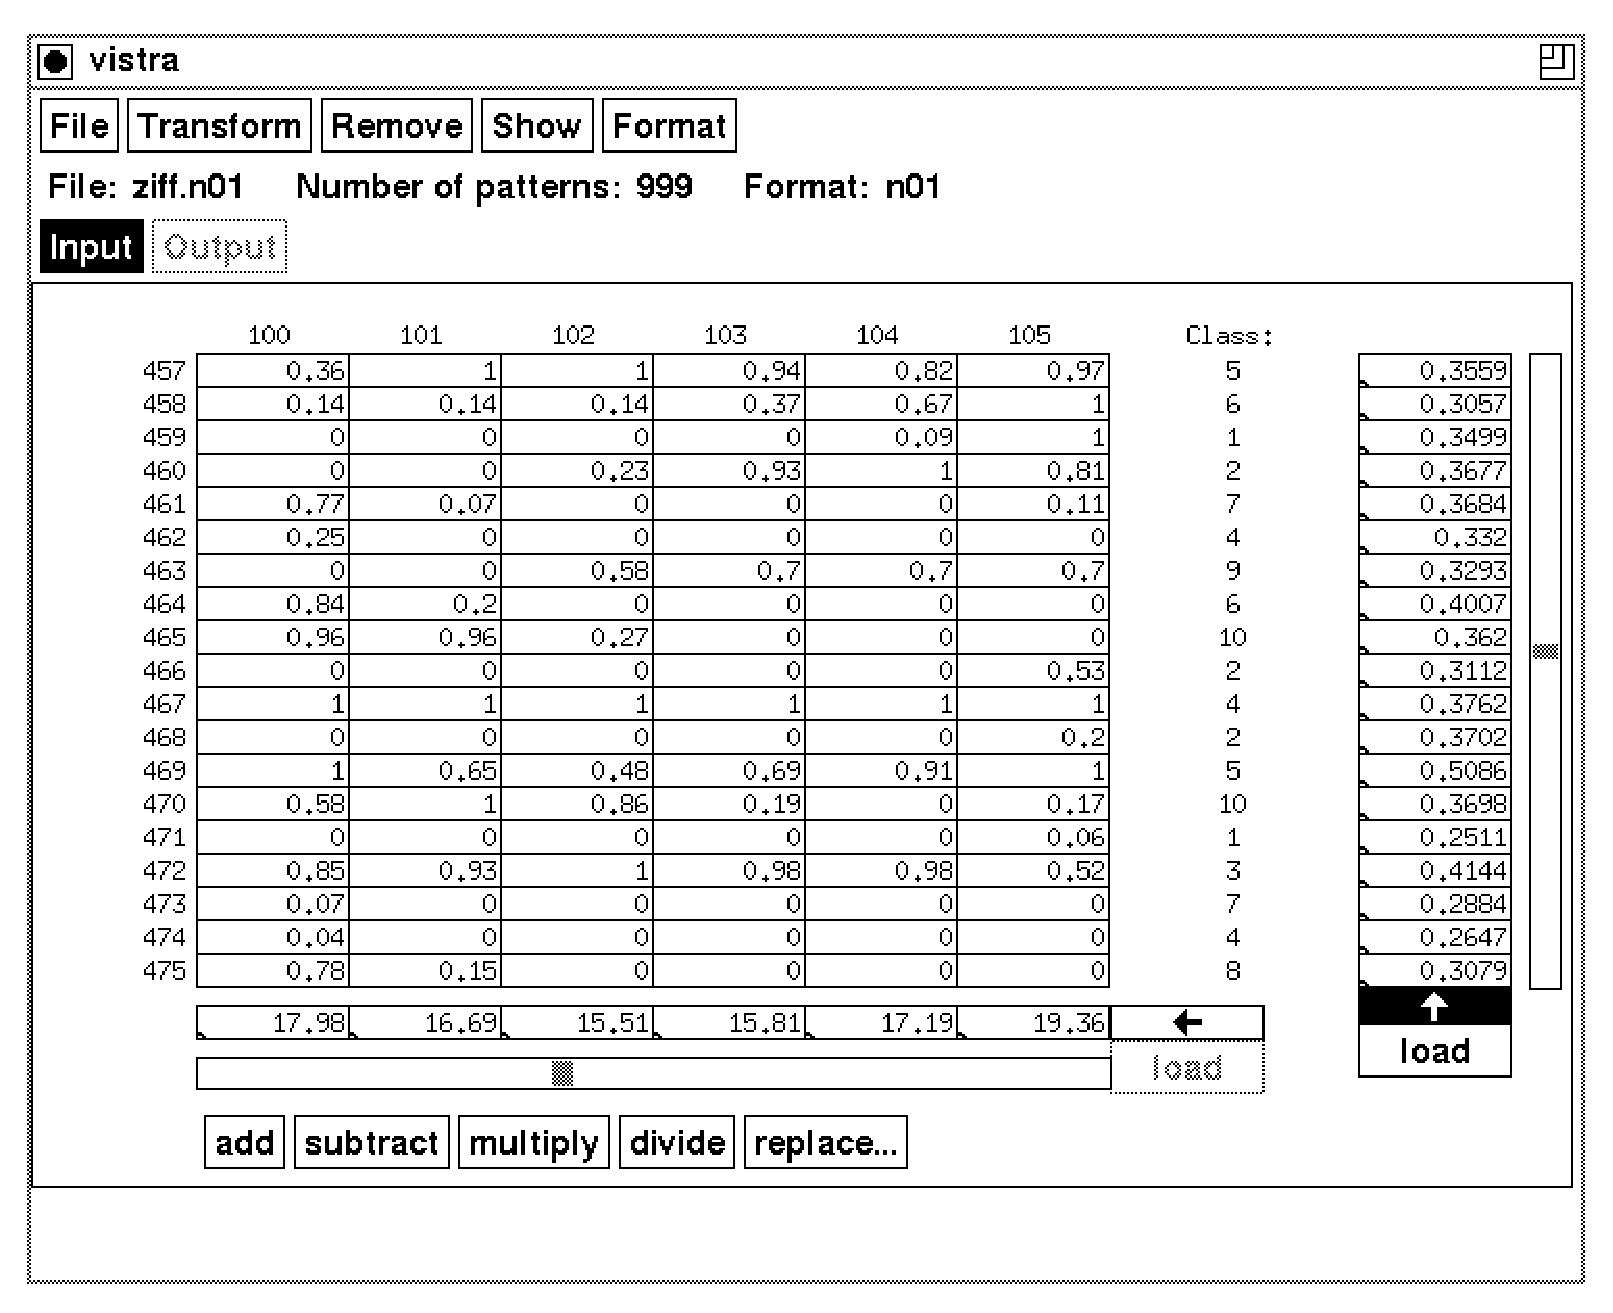
\psfig{file=main.ps,width=\textwidth,height=14cm}}
\caption{\label{hauptfenster} Das Hauptfenster von Vistra}
\end{figure}  

Das Hauptfenster ist in folgende Zonen eingeteilt:
\begin{itemize}
\item Direkt unter der Titelleiste befindet sich die {\bf Men"uleiste}, die
Men"u-Buttons f"ur das "`File"'-, "`Transform"'-, "`Remove"'-, "`Show"'- und 
"`Format"'-Men"u enth"alt.

\item Unterhalb der Men"uleiste folgt eine {\bf Info-Zeile}, die den Namen der
momentan geladenen Trainingsvektor-Datei, die Anzahl der Trainingsvektoren
sowie das momentan ausgew"ahlte Dateiformat anzeigt.

\item Es folgen {\bf zwei Buttons}, die mit "`Input"' bzw.~"`Output"' 
bezeichnet sind. 
Da im Hauptfenster immer nur ein Satz von Vektoren bearbeitet werden kann,
dienen diese Buttons zum Umschalten zwischen Eingabe- und Ausgabevektoren.
"Uber den Men"upunkt "`Input/output vectors"' des "`Show"'-Men"us
kann jedoch ein zweites Fenster ge"offnet werden, in dem immer diejenigen
Vektoren angezeigt werden, die momentan nicht im Hauptfenster bearbeitet 
werden (siehe auch Abschnitt~\ref{ssw}).
Ein Mausklick auf den "`Input"'- bzw. den "`Output"'-Button bewirkt 
ein Austauschen der beiden Fensterinhalte.

\item Ein {\bf Spreadsheet}, das entweder die Eingabe- oder die
Ausgabevektoren enth"alt.
Jede Zeile des Gitters entspricht einem Vektor.
Die Nummern der zum jeweiligen Zeitpunkt sichtbaren Vektoren sind
links neben dem Gitter angebracht.
Unmittelbar oberhalb des Gitters stehen die Nummern der sichtbaren
Dimensionen. \\
In Abbildung~\ref{hauptfenster} werden z.B. momentan die Dimensionen
100 bis 105 der Vektoren 457 bis 475 angezeigt.
Mithilfe der vertikalen bzw.~der horizontalen Scrollbars rechts 
bzw.~unterhalb des Gitters, k"onnen alle Vektorelemente bequem 
durchgebl"attert werden.

\begin{sloppypar}
Unmittelbar rechts neben dem Spreadsheet ist eine Spalte mit der
"Uberschrift "`class:"' zu sehen.
Sie enth"alt die Namen bzw.~Symbole der Klassen, denen die Vektoren
der entsprechenden Zeilen angeh"oren.
Sind keine Klassensymbole geladen, so sind an dieser Stelle die
zugeh"origen Klassennummern aufgef"uhrt. 
\end{sloppypar}

\item Direkt unterhalb bzw.~rechts neben dem Spreadsheet befinden sich 
{\bf horizontale bzw.~vertikale Skalarfelder}.
Sie dienen \ldots

\begin{enumerate}
\item zur Anzeige von Skalar-Werten, die aus den Zeilen-
bzw.~Spaltenvektoren des Spreadsheets abgeleitet werden.
Die vertikalen Felder werden dabei mit Skalaren gef"ullt, die
sich aus den Zeilenvektoren, also Eingabe- oder Ausgabevektoren,
ergeben.
Die horizontalen Felder beziehen sich hingegen auf die Spaltenvektoren
des Spreadsheets und enthalten daher Informationen "uber die einzelnen
Dimensionen der Vektoren.
\item als skalare Operanden zur Durchf"uhrung von Operationen
mit den Vektoren der Spreadsheet (Zeilen- oder Spaltenvektoren).
\end{enumerate}

Immer wenn neue Trainingsvektoren geladen werden bzw. von Eingabe- auf
Ausgabevektoren umgeschaltet wird (oder umgekehrt), werden alle 
vertikalen und horizontalen Skalarfelder auf den Wert "`0"' gesetzt.
Sp"ater k"onnen diese Felder auf zwei Arten mit Werten gef"ullt werden:

\begin{itemize}
\item von Hand mithilfe der Tastatur (dazu mu"s der Maus-Zeiger "uber
dem Eingabefeld stehen).
\item "uber einen Men"upunkt des "`Load"'-Men"us.
\end{itemize}

"Uber das "`Load"'-Men"u k"onnen Mittelwerte, Minima, Standardabweichungen
etc. von Vektoren oder Dimensionen berechnet werden.
Eine vollst"andige Liste der angebotenen Funktionen ist im
Abschnitt~\ref{loadmenu} zu finden.
Die Pfeile, die in Richtung der Skalarfelder zeigen, fungieren als
Schalter, mit denen zwischen den vertikalen und horizontalen Feldern
mittels Mausklick umgeschaltet wird.

Sind beispielsweise die vertikalen Felder selektiert, so beziehen sich
die Funktionen des "`Load"'-Men"us auf die Zeilen der Spreadsheet.
Die Minimum-Funktion des "`Load"'-Men"us w"urde die vertikalen Skalarfelder
mit dem jeweiligen minimalen Element des zugeh"origen Eingabe- bzw.
Ausgabevektors laden. 
Sind hingegen die horizontalen Felder ausgew"ahlt, so w"urden sie 
nach Ausf"uhrung der Minimum-Funktion die minimalen Elemente der einzelnen 
Dimensionen enthalten.

\item Mithilfe der {\bf Skalaroperations-Buttons} direkt unterhalb der 
horizontalen Scrollbar
werden die Zeilen- bzw.~Spaltenvektoren mit den Inhalten der vertikalen
bzw.~horizontalen Skalarfelder kombiniert.
Auch hier mu"s die Richtung der Operation vorher durch die Pfeile
eingestellt werden.
Sind die vertikalen Skalarfelder selektiert, so wird der $i$-te 
Zeilenskalar f"ur die Operation mit dem $i$-ten Zeilenvektor 
verwendet.
Sind hingegen die horizontalen Skalarfelder selektiert, so werden die
Spaltenskalare mit den Spaltenvektoren der Spreadsheet kombiniert.  
Folgende Vektor--Skalar Operationen sind m"oglich: 

\begin{tabular}{ll}
{\bf "`add"'} & elementweise Addition des Skalars \\
{\bf "`subtract"'} & elementweise Subtraktion des Skalars \\
{\bf "`multiply"'} & elementweise Multiplikation des Skalars \\
{\bf "`divide"'} & elementweise Division durch den Skalar \\
{\bf "`replace\ldots"'} & Ersetzen eines bestimmten Elements durch den Skalar \\
\end{tabular}

Im Falle von "`replace\ldots"' "offnet sich eine Dialogbox, in der
die Nummer des zu ersetzenden Elements angegeben werden mu"s.
Die "`replace\ldots"'-Funktion entspricht praktisch dem Ersetzen
einer Zeile bzw.~Spalte des Spreadsheets durch die Inhalte der horizontalen
bzw.~vertikalen Skalarfelder.

\item Der Platz unterhalb der Skalaroperations-Buttons dient zur
Anzeige von Mitteilungen "uber Operationen, Berechnungen usw., die
Vistra momentan durchf"uhrt.

"`Loading patterns\ldots"' beispielsweise besagt,
da"s Vistra zur Zeit eine Trainingsvektor-Datei einliest und deshalb
mit weiteren Benutzereingaben gewartet werden sollte.
\end{itemize}

Au"ser den Vektor--Skalar Operationen werden alle Aktionen des Hauptfensters
"uber entsprechende Men"upunkte aufgerufen.
Die folgenden Abschnitte beschreiben alle Aktionen Men"u f"ur Men"u. 
Generell gilt, da"s Operationen, deren Bezeichnungen auf "`\ldots"' enden, 
nicht sofort ausgef"uhrt werden, sondern zun"achst Dialogboxen "offnen,
in denen der Benutzer zus"atzliche Angaben zur Operation machen mu"s.  

\subsection{Das "`Load"'-Men"u}
\label{loadmenu}

Wie bereits erw"ahnt, dient das "`Load"'-Men"u zum Laden der
vertikalen oder der horizontalen Skalarfelder.
Mithilfe der beiden Pfeile k"onnen die zu ladenden Felder
ausgew"ahlt werden.
Unter jedem Pfeil befindet sich ein mit "`load"' gekennzeichneter
Men"ubutton, "uber den das "`Load"'-Men"u aufgerufen werden kann.

"Uber das "`Load"'-Men"u k"onnen sowohl skalare Werte zu den einzelnen
Vektoren bzw. Dimensionen bestimmt werden als auch globale Werte,
die von {\sl allen} Vektoren abh"angen (wie z.B. das minimale Element aller
Vektoren). 

Die ersten sieben Men"upunkte berechnen die Skalare aus den zugeh"origen
Zeilenvektoren (falls die vertikalen Felder selektiert sind), oder
aus den Spaltenvektoren des Spreadsheets
(falls die horizontalen Felder selektiert sind).  

\begin{samepage}
Sie lauten: \\
\begin{tabular}{lp{10.5cm}}
{\bf Men"upunkt} & {\bf geladen wird\ldots} \\[1ex]
"`minimum"' & das kleinste Element des Vektors \\
"`maximum"' & das gr"o"ste Element des Vektors \\
"`average"' & der Mittelwert der Vektorelemente \\
"`length"' & die L"ange des Vektors \\
"`standard deviation"' & die Standardabweichung $\sigma$ des 
Vektors $v$: \newline
\vspace{1ex}
\[ \sigma(v) = \sqrt{\frac{1}{dims} \sum_{i=1}^{dims} 
(v_{i} - \overline{v})^{2}} \]
\vspace{1ex}
\begin{tabbing}
$dims$ \qquad \= Dimensionalit"at von $v$ \\
$v_{i}$ \> $i$-tes Element von $v$ \\
$\overline{v}$ \> Mittelwert von $v$ 
\end{tabbing} \\
"`sum"' & die Summe aller Elemente des Vektors \\
"`pattern\ldots"' & das $i$-te Element des Vektors, wobei $i$ durch
den Benutzer in einer Dialogbox festgelegt wird 
\end{tabular}
\end{samepage}

Die n"achsten f"unf Men"upunkte f"ullen alle horizontalen bzw.~vertikalen
Skalarfelder mit einer Konstanten: \\

\nopagebreak
\begin{tabular}{lp{9.5cm}}
{\bf Men"upunkt} & {\bf geladen wird\ldots} \\[1ex]
"`overall minimum"' & das kleinste Element {\sl aller} Vektoren \\
"`overall maximum"' & das gr"o"ste Element {\sl aller} Vektoren \\
"`overall average"' & der Mittelwert der Elemente {\sl aller Vektoren} \\
"`overall std dev"' & die globale Standardabweichung $\sigma_{global}$
der Elemente {\sl aller} Vektoren $v_{i}$: \newline
\vspace{1ex}
\[ \sigma_{global} = \sqrt{\frac{1}{n\cdot dims} \sum_{i=1}^{n}
\sum_{j=1}^{dims} (v_{ij} - \overline{v})^{2}} \] 
\vspace{1ex}
\begin{tabbing}
$dims$ \qquad \= Dimensionalit"at der Vektoren $v_{i}$ \\
$n$ \> Anzahl der Vektoren in dem Spreadsheet \\
$v_{ij}$ \> $j$-tes Element des Vektors $v_{i}$ \\
$\overline{v}$ \> globaler Mittelwert ("`overall average"')      
\end{tabbing} \\
"`constant\ldots"' & eine beliebige Konstante, die vom Benutzer in einer 
Dialogbox eingegeben wird 
\end{tabular}

\subsection{Das "`Format"'-Men"u}

Vistra kann eine Vielzahl von Dateiformaten f"ur Trainingsvektoren lesen
und schreiben.
Neben dem LVQ- und dem N01-Format, die standardm"a"sig vorhanden sind,
handelt es sich um benutzerdefinierte ASCII-Formate, 
um die Vistra erweitert werden kann (wie in Kapitel~\ref{fdl} beschrieben).
Beim Lesen bzw.~Schreiben von Trainingsvektoren mu"s der Benutzer daher
das zu verwendende Format festlegen.
Dies geschieht "uber das "`Format"'-Men"u, in dem die Namen aller
dem Programm bekannten Formate aufgelistet sind.
 
Zu jedem Zeitpunkt ist ein Format selektiert und durch einen Haken links
vom Namen gekennzeichnet.
Zus"atzlich wird das ausgew"ahlte Format auch in der Info-Zeile angezeigt.
Die ersten drei Men"upunkte lauten "`see suffix"', "`lvq"' und "`n01"'.
"`see suffix"' bezeichnet hierbei kein bestimmtes Format, sondern legt fest, 
da"s das zu verwendende Format jeweils durch
die Endung des Dateinamens bestimmt ist.
Ist "`see suffix"' selektiert und soll z.B.~die Vektordatei "`ziffern.n01"'
geladen werden, so geht Vistra davon aus, da"s diese Datei im N01-Format
vorliegt.

Ab dem vierten Men"upunkt erscheinen die Namen der benutzerdefinierten
Formate.
Als Namen dienen hierbei die Dateinamen der FDL-Beschreibungen ohne
die Endung "`.fmt"'.  
 
\subsection{Das "`File"'-Men"u}

"Uber das "`File"'-Men"u k"onnen alle Vistra-Funktionen aufgerufen werden,
die mit dem Lesen oder dem Schreiben von Dateien zutun haben. 

\begin{description}
\item["`Load patterns\ldots"':] \mbox{} \\  
Lade neue Trainingsvektoren. \\
Es "offnet sich eine Dialogbox, in der der Name der Vektor-Datei
anzugeben ist.
Ist im "`Format"'-Men"u "`see suffix"' eingestellt, so gibt die Endung
des Dateinamens an, welches Format die Datei besitzt.

\item["`Write patterns\ldots"':] \mbox{} \\
Schreibe die bearbeiteten Trainingsvektoren in eine 
Trai\-nings\-vek\-tor-Datei. \\
Es "offnet sich eine Dialogbox, in der der Name der zu schreibenden Datei
anzugeben ist.
Ist im "`Format"'-Men"u "`see suffix"' eingestellt, so gibt die Endung
des Dateinamens an, in welchem Format die Trainingsvektoren geschrieben 
werden.

\item["`Load symbols\ldots"':] \mbox{} \\
Lade eine neue Symboltabelle. \\
Die Funktion ordnet den Klassennummern neue Symbole zu.
Die Symbole m"ussen dazu in einer Symboltabellen-Datei untergebracht sein.
Eine solche Symboltabellen-Datei hat Zeilenstruktur, wobei
die erste Zeile das erste Symbol enth"alt, die zweite Zeile das
zweite Symbol etc. 
Eine genaue Beschreibung des Formats findet sich im Abschnitt~\ref{symtab}.
Der Namen der Symboltabellen-Datei wird "uber eine Dialogbox vom Benutzer
erfragt.

Am Beispiel des xor-Problems soll dieser Proze"s veranschaulicht
werden. \\
Folgende Daten seien vor dem Laden im Speicher: 

\begin{tabular}{ccc}
{\sl Trainingsvektor} & {\sl Klassennummer} & {\sl Klassensymbol} \\[1ex]
{\tt 0 0} & {\tt 1} & {\tt NULL} \\
{\tt 0 1} & {\tt 2} & {\tt EINS} \\
{\tt 1 0} & {\tt 2} & {\tt EINS} \\
{\tt 1 1} & {\tt 1} & {\tt NULL} \\
\end{tabular}  

Die Symbole {\tt NULL} und {\tt EINS} sollen nun durch die Symbole
{\tt FALSE} und {\tt TRUE} ersetzt werden.
Dazu wird eine Symboltabellen-Datei mit folgendem Inhalt geladen: 
\begin{verbatim}
FALSE
TRUE
\end{verbatim}
Nach dem Laden liegen folgende Daten vor: 

\begin{tabular}{ccc}
{\sl Trainingsvektor} & {\sl Klassennummer} & {\sl Klassensymbol} \\[1ex]
{\tt 0 0} & {\tt 1} & {\tt FALSE} \\
{\tt 0 1} & {\tt 2} & {\tt TRUE} \\
{\tt 1 0} & {\tt 2} & {\tt TRUE} \\
{\tt 1 1} & {\tt 1} & {\tt FALSE} \\
\end{tabular}  

Mit der "`Load symbols\ldots"'-Funktion k"onnen Symbole nicht nur
ersetzt werden, sondern "uberhaupt erst einmal geladen werden.
Dies ist, wie bereits erw"ahnt, f"ur Trainingsvektoren sinnvoll, die 
im N01-Format geladen wurden, da das Format nur Klassennummern enth"alt.

Enth"alt eine Symboltabellen-Datei weniger Symbole als unterschiedliche
Klassen existieren, so erscheint eine Fehlermeldung.

\item["`Write symbols\ldots"':] \mbox{} \\
Schreibe die Symboltabelle in eine Symboltabellen-Datei. \\
Der Namen dieser Datei wird vom Benutzer "uber eine Dialogbox erfragt.
Ausgegeben werden die Klassensymbole oder, falls keine geladen sind,
die Ausgabevektoren (siehe Abschnitt~\ref{symtab}).
Existieren weder Symbole noch Ausgabevektoren, so werden einfach die
Klassennummern geschrieben.
  
\item["`Write to log file"':] \mbox{} \\ 
Dieser Men"upunkt stellt einen Schalter 
dar, wobei ein Haken anzeigt, ob die Funktion ein- oder abgeschaltet ist.
Solange sie eingeschaltet ist, werden alle Transformationen, die
auf den Eingabe- oder Ausgabevektoren durchgef"uhrt werden, in einer
LOG-Datei festgehalten.
Zu einem sp"ateren Zeitpunkt k"onnen die durchgef"uhrten Transformationen
dann mit denselben oder anderen Trainingsvektoren wiederholt werden.
Die Funktion kann w"ahrend einer Sitzung beliebig ein- oder ausgeschaltet
werden, wobei immer nur ans Ende der LOG-Datei angeh"angt wird.

Der Namen der LOG-Datei ist {\it pattern\_file\_name}{\tt\/.log},
wobei {\it pattern\_file\_name} den Namen der momentan  
geladenen Trainingsvektor-Datei repr"asentiert.
Sie wird daher in das Verzeichnis der Vektordatei gestellt.  
Das Format der LOG-Dateien wird ausf"uhrlich 
im Kapitel~\ref{log} behandelt.

\item["`Quit"':] \mbox{} \\
Beende Vistra.  
\end{description}

\subsection{Das "`Transform"'-Men"u}

Das "`Transform"'-Men"u enth"alt Funktionen zur Transformation der
Eingabevektoren oder der Ausgabevektoren, je nachdem, welche gerade
im Hauptfenster bearbeitet werden.
Es werden immer {\sl alle} Vektoren transformiert, das gezielte
Transformieren eines einzelnen Vektors ist weder zweckm"a"sig noch erlaubt. \\ 
Folgende Transformationen sind m"oglich:

\begin{description}
\item["`HLOG"':] \mbox{} \\
Es wird eine halblogarithmische 
Transformation mit den Vektoren durchgef"uhrt. \\
Sie kann nur auf Vektoren ausgef"uhrt werden, die eine quadratische
Anzahl von Dimensionen besitzen. 

Bei der Bilderkennung mit Hilfe neuronaler Netze bereiten gedrehte Objekte
besonders gro"se Probleme.
Eine Abhilfe kann die sogenannte halblogarithmische Transformation 
schaffen.
Die Vektorelemente (Bildpunkte) werden durch diese Transformation nicht
ver"andert, sondern lediglich anders angeordnet.

Man kann sich die Transformation folgenderma"sen vorstellen: \\
Man legt $b$ konzentrische Kreise mit exponentiell wachsenden Radien um den
Mittelpunkt des Bildes, wobei $b$ die Seitenl"ange des quadratischen Bildes 
in Bildpunkten ist.
Der Radius $r_i$ des $i$-ten Kreises ($i=0,1,\ldots,b-1$) betr"agt:

\[ r_i = \left( \frac{b}{2}\right)^{\frac{i}{b-1}} \qquad \mbox{Bildpunkte} \] 

Legt man nun Geraden durch den Mittelpunkt, die jeweils einen Winkel
von $\frac{2\pi}{b}$ ein\-schlie"sen, so wird die erste Spalte des neuen
Bildes aus den Bildpunkten des Originals gebildet, die im 
Gegenuhrzeigersinn unter den Schnittpunkten dieser Geraden mit dem innersten
Kreis liegen.
Die zweite Spalte erh"alt man aus den Schnittpunkten mit dem zweitinnersten 
Kreis usw.
Die Schnittpunkte mit dem "au"sersten Kreis liefern schlie"slich die Elemente 
der letzten Spalte des transformierten Bildes. 

Durch die halblogarithmische Transformation wird erreicht, da"s
Drehungen von Objekten im Original   
zu Verschiebungen im transformierten Bild f"uhren.
Verschiebungen k"onnen von neuronalen Netzen jedoch wesentlich leichter
erkannt werden.

\item["`FFT"':] \mbox{} \\
Es wird eine diskrete eindimensionale 
Fourier Transformation (FFT) auf den Vektoren durchgef"uhrt.
Diese Transformation ist nur f"ur Vektoren zul"assig, die $2^{n}$ 
($n \geq 1$) Dimensionen besitzen.

Bei der FFT handelt es sich um eine komplexwertige Vektorfunktion.
Bevor eine FFT auf einem Vektor $v$ durchgef"uhrt wird, m"ussen die
Vektorelemente $v_{i}$ deshalb zun"achst in komplexe Zahlen 
$(v_{i,real},v_{i,imag})$ "uberf"uhrt werden. \\
Dies geschieht in Vistra wie folgt:

\begin{tabular}{@{\hspace*{1cm}}lcl}
$v_{i,real}$ & := & $v_{i}$ \\
$v_{i,imag}$ & := & $0.0$ \\
\end{tabular}

Nach Durchf"uhrung der Fourier Transformation auf dem Vektor $v$
werden die komplexen Vektorelemente wieder in reelle Zahlen umgewandelt:

\hspace*{1cm} $v_{i} := \sqrt{v_{i,real}^{2} + v_{i,imag}^{2}}$

Die diskrete eindimensionale Fourier Transformation ist ausf"uhrlich
in \cite{jaehne} beschrieben. 

\item["`PCA"':] \mbox{} \\ 
Auf den Vektoren wird eine 
Haupt\-achsen-Trans\-form\-ation 
({\bf P}rinciple {\bf C}om\-po\-nent {\bf A}na\-ly\-sis) 
durchgef"uhrt. \\
F"ur eine Beschreibung sei auf \cite{hertz} oder \cite{bronstein} verwiesen. 

Vistra verwendet zur Durchf"uhrung der PCA-Transformation das 
Programm "`pca"', das Trainingsvektoren im LVQ-Format liest, die PCA
durchf"uhrt und die transformierten Vektoren anschlie"send im LVQ-Format 
nach stdout schreibt. 

Vistra schreibt daher in einem ersten Schritt die Trainingsvektoren 
im LVQ-Format in eine tempor"are Datei, ruft anschlie"send das Programm 
"`pca"' mit dieser Datei als Parameter auf, lenkt die Ausgabe auf 
eine weitere tempor"are Datei um und liest diese 
schlie"slich wieder im LVQ-Format ein.

\item["`Normalize"':] \mbox{} \\
Alle Vektoren des Spreadsheets werden 
normalisiert, d.h.~jeder Vektor $v$ 
wird elementweise durch seine L"ange $|v|$ dividiert, so da"s jeder Vektor
anschlie"send die L"ange $|v|=1$ besitzt:
 
\[ v := \frac{v}{|v|} \]

Diese Transformation kann auch leicht mithilfe der Skalarfelder 
durchgef"uhrt werden.
Zuerst l"adt man die vertikalen Skalarfelder mit den L"angen der Vektoren
(Men"upunkt "`length"' des "`Load"'-Men"us).
Anschlie"send wird der "`divide"'-Button gedr"uckt.

\item["`Scale\ldots"':] \mbox{} \\
Die Elemente aller Vektoren werden 
auf einen neuen Wertebereich skaliert, der in einer Dialogbox anzugeben ist. 

Die Skalierung erfolgt derart, da"s das kleinste Element des Spreadsheets
("`overall minimum"') auf die untere Intervallgrenze und das gr"o"ste
("`overall maximum"') auf die obere Intervallgrenze abgebildet wird.

\item["`Randomize"':] \mbox{} \\
Die Reihenfolge der Trainingsvektoren wird willk"urlich ver"andert.

\item["`Expand with class vector"':] \mbox{} \\
Jeder Vektor des Spreadsheets wird mit seinem Klassenvektor erweitert. 

Unter Klassenvektor versteht man dabei einen Vektor bestehend aus Nullen
und Einsen, wobei die Anzahl der Dimensionen der Anzahl unterschiedlicher
Klassen entspricht. 
Das $i$-te Element des Klassenvektors ist genau dann 1, wenn der
Trainingsvektor die Klassennummer $i$ besitzt, sonst 0. 

Das Erweitern durch die Klassenvektoren soll am xor-Beispiel veranschaulicht
werden. \\
Links sind die Vektoren vor und rechts nach der Transformation zu
sehen: 

\nopagebreak
\begin{tabular}{ccc}
{\sl Eingabevektoren vorher} & {\sl Klassen-Nr.} & 
{\sl Eingabevektoren nachher} \\[1ex] 
{\tt 0 0} & {\tt 1} & {\tt 0 0 1 0} \\  
{\tt 0 1} & {\tt 2} & {\tt 0 1 0 1} \\  
{\tt 1 0} & {\tt 2} & {\tt 1 0 0 1} \\  
{\tt 1 1} & {\tt 1} & {\tt 1 1 1 0} \\  
\end{tabular}
 
\item["`Expand with output vector"':] \mbox{} \\
Diese Transformation kann nur durchgef"uhrt werden, wenn 
Ausgabevektoren existieren.
Die Vektoren des Spreadsheets werden mit den Elementen des 
zugeh"origen Ausgabevektors erweitert.

\item["`Refresh class numbers"':] \mbox{} \\
Es werden die Klassennummern anhand der Ausgabevektoren neu berechnet. \\ 
Diese Funktion kann nur aufgerufen werden, wenn keine Klassensymbole geladen
sind.

Trainingsvektoren mit gleichen Ausgabevektoren erhalten die gleichen
Klassennummern.
Die vergebenen Nummern sind 1, 2,\ldots, $n$ , wobei $n$ 
der Anzahl unterschiedlicher Ausgabevektoren entspricht.
\end{description}
 
\subsection{Das "`Remove"'-Men"u}

Das "`Remove"'-Men"u h"alt Funktionen bereit, mit denen Trainingsvektoren
oder bestimmte Dimensionen der Vektoren entfernt werden k"onnen:

\begin{description}
\item["`Dimensions\ldots"':] \mbox{} \\
Es wird ein Bereich von Dimensionen (also Spalten des Spreadsheets) entfernt. \\
Dazu "offnet sich eine Dialogbox, in der die erste und die letzte der
zu entfernenden Dimensionen anzugeben ist.
Es k"onnen nicht alle Dimensionen entfernt werden.

\item["`Constant dims"':] \mbox{} \\
Es werden alle konstanten Dimensionen, also alle Spalten des
Spread\-sheets, 
in denen alle Elemente die gleichen Werte besitzen, entfernt.
Sind alle Dimensionen konstant, so kann die Operation nicht
ausgef"uhrt werden.

\item["`Vectors\ldots"':] \mbox{} \\
Es wird eine Reihe von Trainingsvektoren entfernt. \\
In einer Dialogbox ist der Nummernbereich der zu entfernenden Vektoren
zu spezifizieren.
Es k"onnen jedoch nicht alle Trainingsvektoren gel"oscht werden.
\end{description}

\subsection{Das "`Show"'-Men"u} 

Neben dem Hauptfenster existieren weitere Fenster, die alle "uber
einen entsprechenden Men"upunkt des "`Show"'-Men"us ge"offnet werden. \\
Folgende Men"upunkte stehen zur Verf"ugung:

\nopagebreak
\begin{description}
\item["`Graphics"':] \mbox{} \\
Es wird ein Graphik-Fenster ge"offnet. 
Ein Graphik-Fenster kann wahlweise die Ein\-ga\-be- oder die Ausgabevektoren
in einer von f"unf verschiedenen Darstellungsarten graphisch darstellen.
Es k"onnen beliebig viele solcher Graphik-Fenster ge"offnet werden.
Dadurch ist es m"oglich, ein und denselben Vektor 
auf mehrere Arten gleichzeitig wiederzugeben.
   
\item["`Statistics"':] \mbox{} \\
Es wird ein Fenster ge"offnet, das statistische Informationen "uber die
geladenen Trai\-nings\-vek\-to\-ren anzeigt.

\item["`Covariance matrix"':] \mbox{} \\
Es wird ein Fenster ge"offnet, 
das die Kovarianzmatrix der im Hauptfenster befindlichen Vektoren
anzeigt.

\item["`Input/output vectors"':] \mbox{} \\
Es wird ein Fenster ge"offnet, in dem die Eingabevektoren oder die
Ausgabevektoren textuell dargestellt werden. 
Dieses Fenster enth"alt immer genau diejenigen Vektoren, die momentan
nicht im Hauptfenster bearbeitet werden.
Auf diese Weise k"onnen zugeh"orige Eingabe- und Ausgabevektoren
gleichzeitig betrachtet werden.
\end{description}

Die folgenden Abschnitte zeigen diese Fenster nun der Reihe nach und
geben Hinweise zu deren Benutzung.
  
\subsection{Die Graphik-Fenster}

Zu jedem Zeitpunkt k"onnen mehrere Graphik-Fenster ge"offnet sein.
Jedes dieser Fenster kann Vektoren in einer der folgenden f"unf
Darstellungsarten graphisch wiedergeben:

\begin{itemize}
\item als Histogramm
\item als Linienzug
\item als Grauwertbild
\item als Farbbild
\item als 2-dimensionale Projektion
\end{itemize} 

Zwischen diesen Darstellungsarten kann beliebig umgeschaltet werden.
Auch die Gr"o"se der Abbildungen kann man innerhalb gewisser Grenzen
ver"andern.
Abbildung~\ref{grayMat} zeigt ein Graphik-Fenster, das momentan 
auf "`gray matrix"' eingestellt ist und einen Vektor als Grauwertbild
darstellt.

\begin{figure}[ht]
\centerline{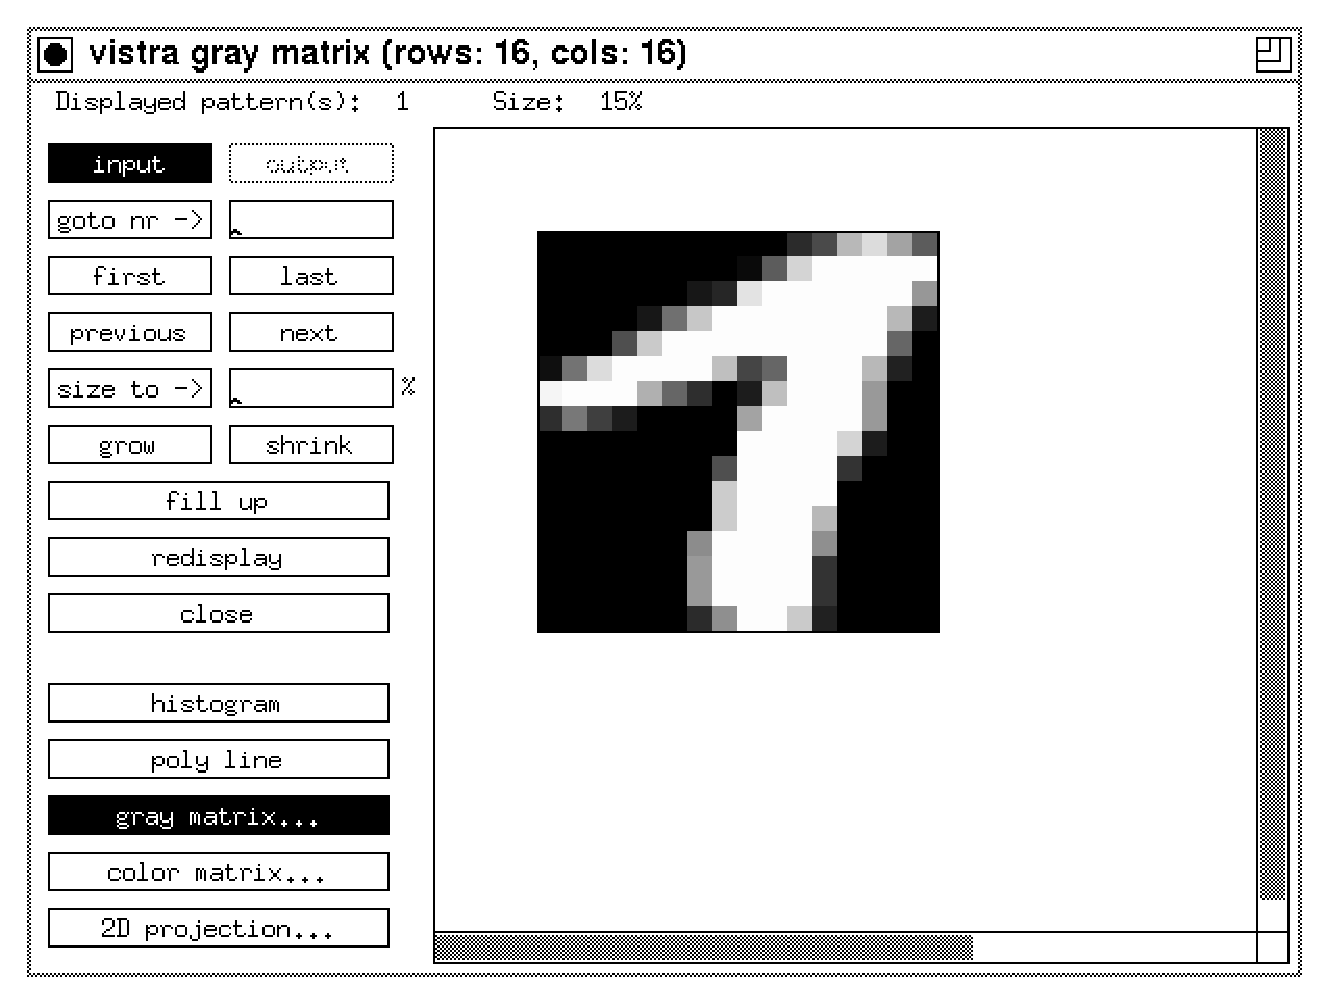
\psfig{file=gray.ps,width=\textwidth,height=10cm}}
\caption{\label{grayMat} Graphik-Fenster mit Grauwertbild}
\end{figure}

Der Titel des Fensters gibt an, welche Darstellungsart momentan gew"ahlt ist.
Unterhalb der Titelleiste erscheint eine Zeile, die Auskunft "uber die
Nummer des abgebildeten Vektors und die Gr"o"se der Abbildung (in \%
der Maximalgr"o"se) gibt.
F"ur die 2-dimensionale Projektion wird anstelle einer Vektor-Nummer
der String "`all"' angezeigt, da diese Darstellungsart alle Vektoren
gemeinsam in einer einzigen Graphik bzw.~Koordinatensystem wiedergibt. 

Am linken Rand des Graphik-Fensters befinden sich eine Reihe von 
Kommando-Buttons.
Durch sie werden Aktionen zum "`Durchbl"attern"' der Vektoren, zur
Ver\-gr"o"ser\-ung/Ver\-kleiner\-ung der Darstellungen oder zum Umschalten
zwischen Eingabe- und Ausgabevektoren bzw.~zum Umschalten zwischen den
verschiedenen Darstellungsarten, ausgef"uhrt. \\
Tabelle~\ref{gwcomms} beschreibt die Buttons des Graphik-Fensters.

\begin{table}[ht]
\begin{tabular}{lp{10.8cm}}
{\bf Button} & {\bf Aktion} \\ \hline
"`input"' & zeige einen Eingabevektor \\
"`output"' & zeige einen Ausgabevektor \\
"`goto nr --$>$"' & zeige den Vektor mit der Nummer, die das Eingabefeld rechts
daneben enth"alt \\
"`first"' & zeige den Vektor Nummer~1 \\
"`last"' & zeige den Vektor mit der h"ochsten Nummer \\
"`previous"' & zeige den vorhergehenden Vektor \\
"`next"' & zeige den n"achsten Vektor \\
"`size to --$>$"' & zeichne die Graphik in $i$ Prozent der Maximalgr"o"se, wobei
$i$ ins Eingabefeld rechts daneben einzutragen ist \\
"`grow"' & vergr"o"sere die Graphik \\
"`shrink"' & verkleinere die Graphik \\
"`fill up"' & nutze den Platz rechts und unterhalb des Diagramms zur 
gleichzeitigen Darstellung weiterer Vektoren.
"Uber jedem Diagramm befindet sich die Nummer des dargestellten Vektors.
Abbildung~\ref{fillup} zeigt ein Graphik-Fenster, das die Vektoren 1 bis 999
als Grauwertbilder minimaler Gr"o"se wiedergibt (1 Pixel pro Vektorelement).
  \\
"`redisplay"' & aktualisiere die Graphik (die dargestellten Vektoren
wurden im Hauptfenster seit dem letzten Zeichnen evtl.~modifiziert;
die graphische Darstellung w"are in diesem Fall veraltet) \\
"`close"' & schlie"se das Graphik-Fenster \\
"`histogram"' & zeige den Vektor als Histogramm \\
"`poly line"' & zeige den Vektor als Linienzug \\
"`gray matrix\ldots"' & zeige den Vektor als Grauwertbild. 
Die Anzahl der Zeilen und Spalten wird "uber eine Dialogbox durch den 
Benutzer festgelegt. \\
"`color matrix\ldots"' & zeige den Vektor als Farbbild.
Die Anzahl der Zeilen und Spalten wird "uber eine Dialogbox durch den
Benutzer festgelegt. \\
"`2D projection\ldots"' & stelle alle Vektoren in einem gemeinsamen
2-dimensionalen Koordinatensystem dar.
Der Benutzer legt in einer Dialogbox fest, welche Dimension die x-Werte
und welche Dimension die y-Werte liefern soll. 
\end{tabular}
\caption{\label{gwcomms} Die Buttons des Graphik-Fensters}
\end{table}

\begin{figure}[ht]
\centerline{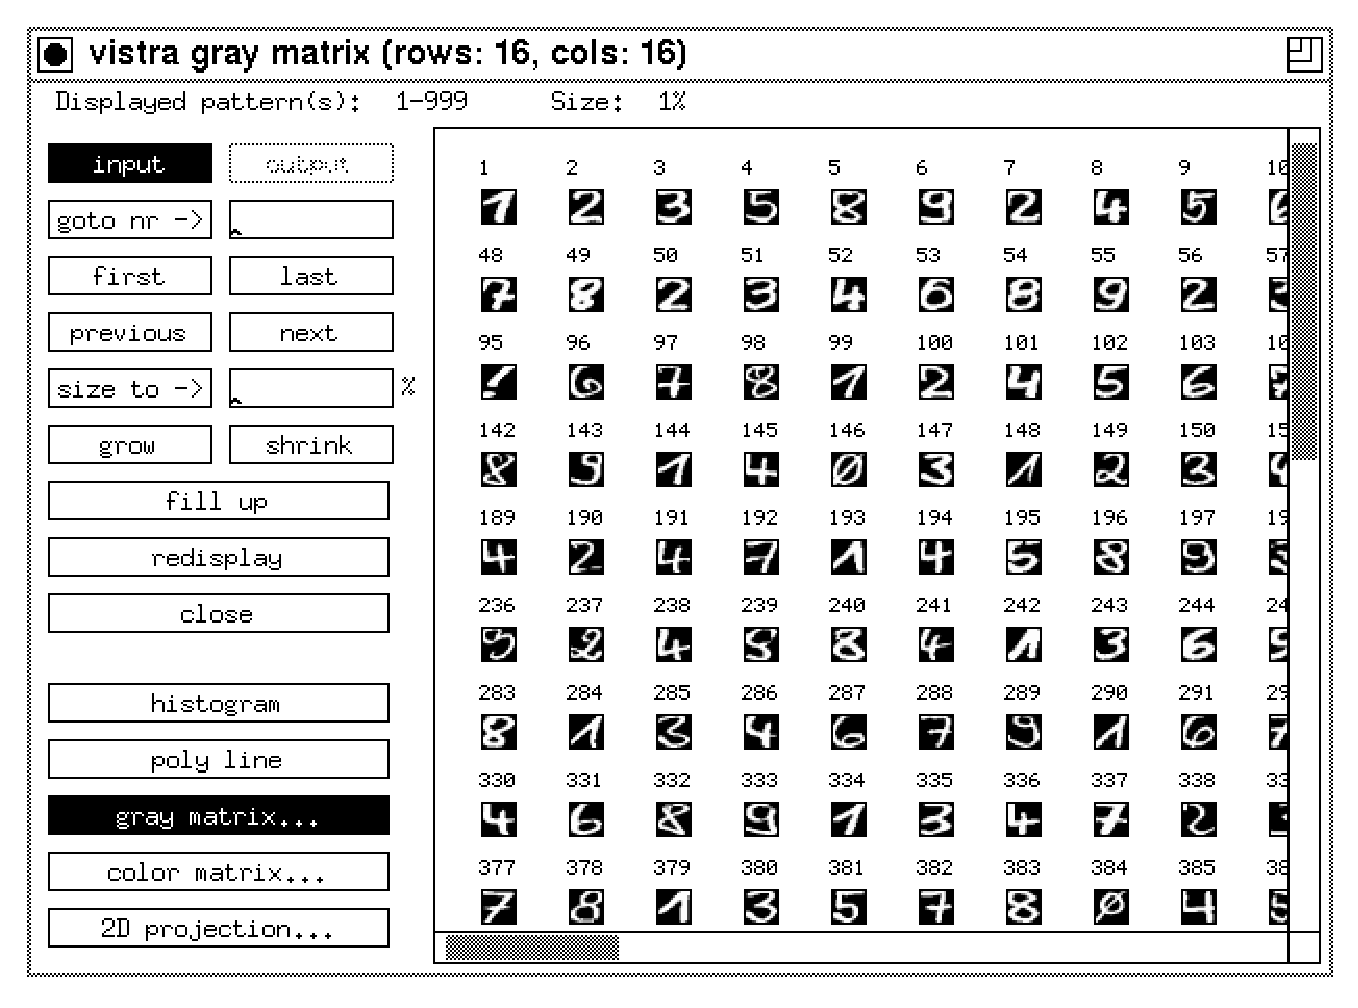
\psfig{file=fillup.ps,width=\textwidth,height=10cm}}
\caption{\label{fillup} Gleichzeitige Darstellung mehrerer Vektoren}
\end{figure}

{\bf WICHTIG:} Auch w"ahrend ein oder mehrere Graphik-Fenster ge"offnet 
sind, k"onnen die Vektoren im Hauptfenster weiterhin bearbeitet
bzw.~transformiert werden.
Aus diesem Grund ist es m"oglich, da"s ein Graphik-Fenster eine 
"`alte Version"' eines Vektors wiedergibt. 
Um sicherzustellen, da"s die Darstellung auf dem neuesten Stand ist,
sollte ein "`redisplay"' durchgef"uhrt werden oder irgendein anderer
Button gedr"uckt werden, der ein Neuzeichnen der Graphik bewirkt
(z.B.~"`next"', "`grow"' etc.). 

\subsection{Die Darstellungsarten}

\subsubsection*{Histogramm}

Ein Histogramm stellt eine Art "`Treppenfunktion"' in einem 
zweidimensionalen Koordinatensystem dar. 
Dabei liefert jedes Element $v_{i}$ des Vektors den Funktionswert 
f"ur den Bereich $[i\!-\!1,i]$ der x-Achse.
Abbildung~\ref{histo} zeigt ein Graphik-Fenster, das ein
Histogramm wiedergibt.
Der dargestellte Vektor besitzt 32 Dimensionen und ist das Ergebnis
einer vorausgegangen Fourier-Transformation.

\begin{figure}[ht]
\centerline{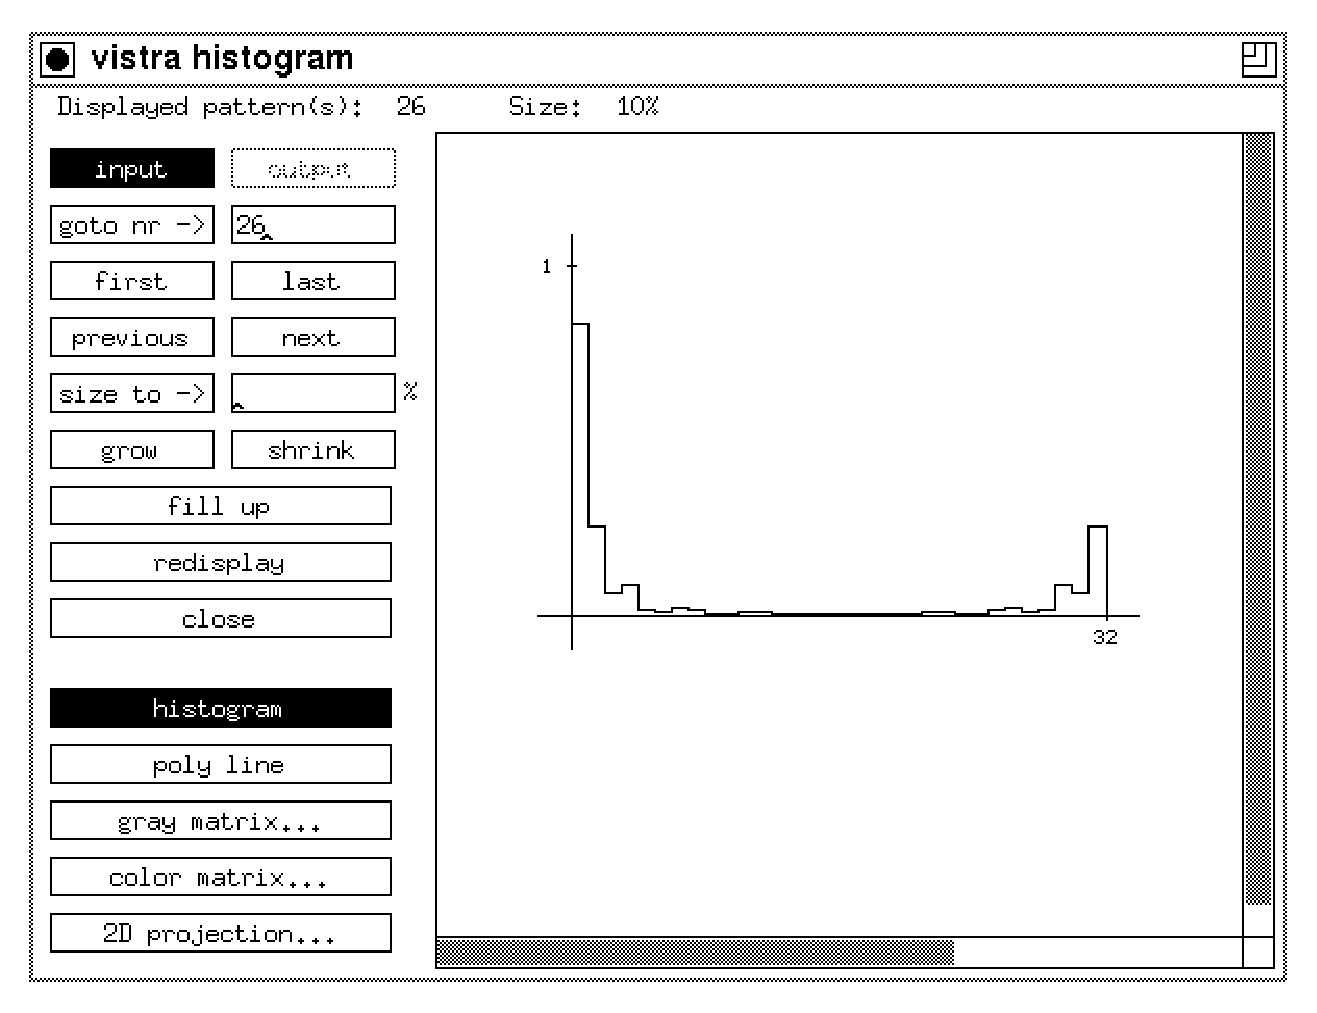
\psfig{file=histo.ps,width=\textwidth,height=10cm}}
\caption{\label{histo} Histogramm-Darstellung eines Vektors}
\end{figure} 

W"ahrend die H"ohe des Histogramms konstant bleibt, kann die Breite
"uber die entsprechenden Buttons des Graphik-Fensters ("`size to --$>$"',
"`grow"' oder "`shrink"') ver"andert werden.
Um die minimale Breite zu erhalten, gibt man als Gr"o"se "`0\%"' an.
Eine L"angeneinheit der x-Achse ist dann 1~Pixel breit.
 
\subsubsection*{Linienzug}

Ein Linienzug ist einem Histogramm sehr "ahnlich. 
Auch er wird in ein zweidimensionales Koordinatensystem gezeichnet.
Die Vektorelemente $v_{i}$ liefern dabei die Punkte $(i,v_{i})$, die
durch Linien verbunden werden.
Abbildung~\ref{poly} zeigt eine Linienzug-Darstellung des Vektors aus
Abbildung~\ref{histo}.

\begin{figure}[ht]
\centerline{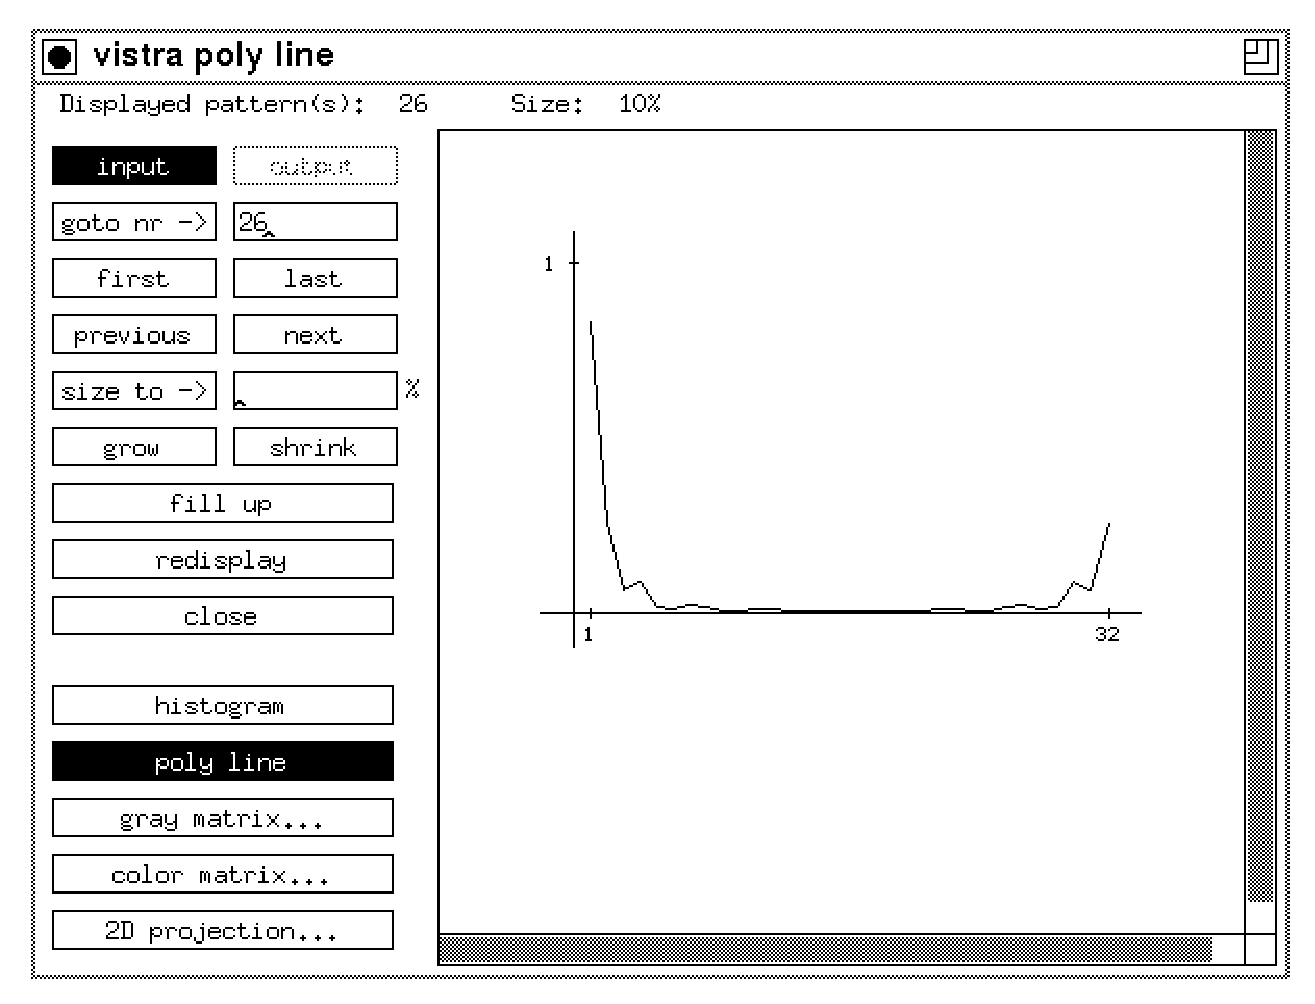
\psfig{file=poly.ps,width=\textwidth,height=10cm}}
\caption{\label{poly} Linienzug-Darstellung eines Vektors}
\end{figure} 

Die x-Achse kann "uber die entsprechenden Buttons des Graphik-Fensters
gedehnt oder geschrumpft werden.
Eine L"angeneinheit der x-Achse ist im Minimalfall genau ein Pixel breit. 

\subsubsection*{Grauwertbild}

Abbildung~\ref{grayMat} zeigte bereits ein Grauwertbild eines Vektors.
Der dargestellte Vektor besitzt 256 Dimensionen, die in eine Matrix
mit 16~Zeilen und 16~Spalten eingeteilt wurden.
Jedes Vektorelement wird durch ein Quadrat repr"asentiert, das in einem
bestimmten Grauton gezeichnet ist.
Das kleinste Element aller Eingabevektoren (bzw.~Ausgabevektoren)
erh"alt dabei die geringste Intensit"at und wird daher schwarz dargestellt.
Das gr"o"ste Element erh"alt die h"ochste Intensit"at und erscheint wei"s.
Werte dazwischen werden je nach Gr"o"se in einem Grauton dargestellt. 

Die Anzahl der Zeilen~bzw.~Spalten der Matrix wird vom Benutzer festgelegt. 
Die Anzahl der Zellen mu"s jedoch mindestens so gro"s wie die Dimensionalit"at
des abzubildenden Vektors sein.
Die ersten Elemente des Vektors werden durch die erste Zeile der Matrix
repr"asentiert, die n"achsten durch die zweite Zeile etc.
"`"Ubersch"ussige"' Zellen werden wei"s dargestellt. 

Die Elemente $v_{1}, \ldots, v_{7}$ eines 7-dimensionalen Vektors w"urden
wie folgt auf eine 3x3-Matrix verteilt werden:

\hspace*{2cm}
\begin{tabular}{|c|c|c|}
\hline $v_{1}$ & $v_{2}$ & $v_{3}$ \\
\hline $v_{4}$ & $v_{5}$ & $v_{6}$ \\
\hline $v_{7}$ & & \\ \hline
\end{tabular}    
 
Die Gr"o"se der quadratischen Zellen kann "uber die entsprechenden Buttons
des Graphik-Fensters ver"andert werden.
Die Minimalgr"o"se betr"agt ein Pixel. 

\subsubsection*{Farbbild}

Die Darstellung eines Vektors als Farbbild erfolgt analog der
Grauwert-Darstellung.
Einziger Unterschied ist die Verwendung des gesamten Farbspektrums
anstelle von Graut"onen.

\subsubsection*{2D-Projektion}

Die 2D-Projektion ist die einzige Darstellungsart, in der
{\it alle} Vektoren in einer einzigen Graphik wiedergegeben sind.
Jeder Vektor wird als ein Punkt in ein zweidimensionales Koordinatensystem
eingetragen.
Der Benutzer legt fest, welche Dimension der Vektoren die x-Werte und
welche die y-Werte liefert.

Abbildung~\ref{proj2D} zeigt ein Beispiel, in dem die Dimensionen~2 und 1
von insgesamt 10~000 Vektoren abgebildet sind.
Die Gr"o"se des Schaubilds kann "uber die entsprechenden Buttons des 
Graphik-Fensters variiert werden.

\begin{figure}[ht]
\centerline{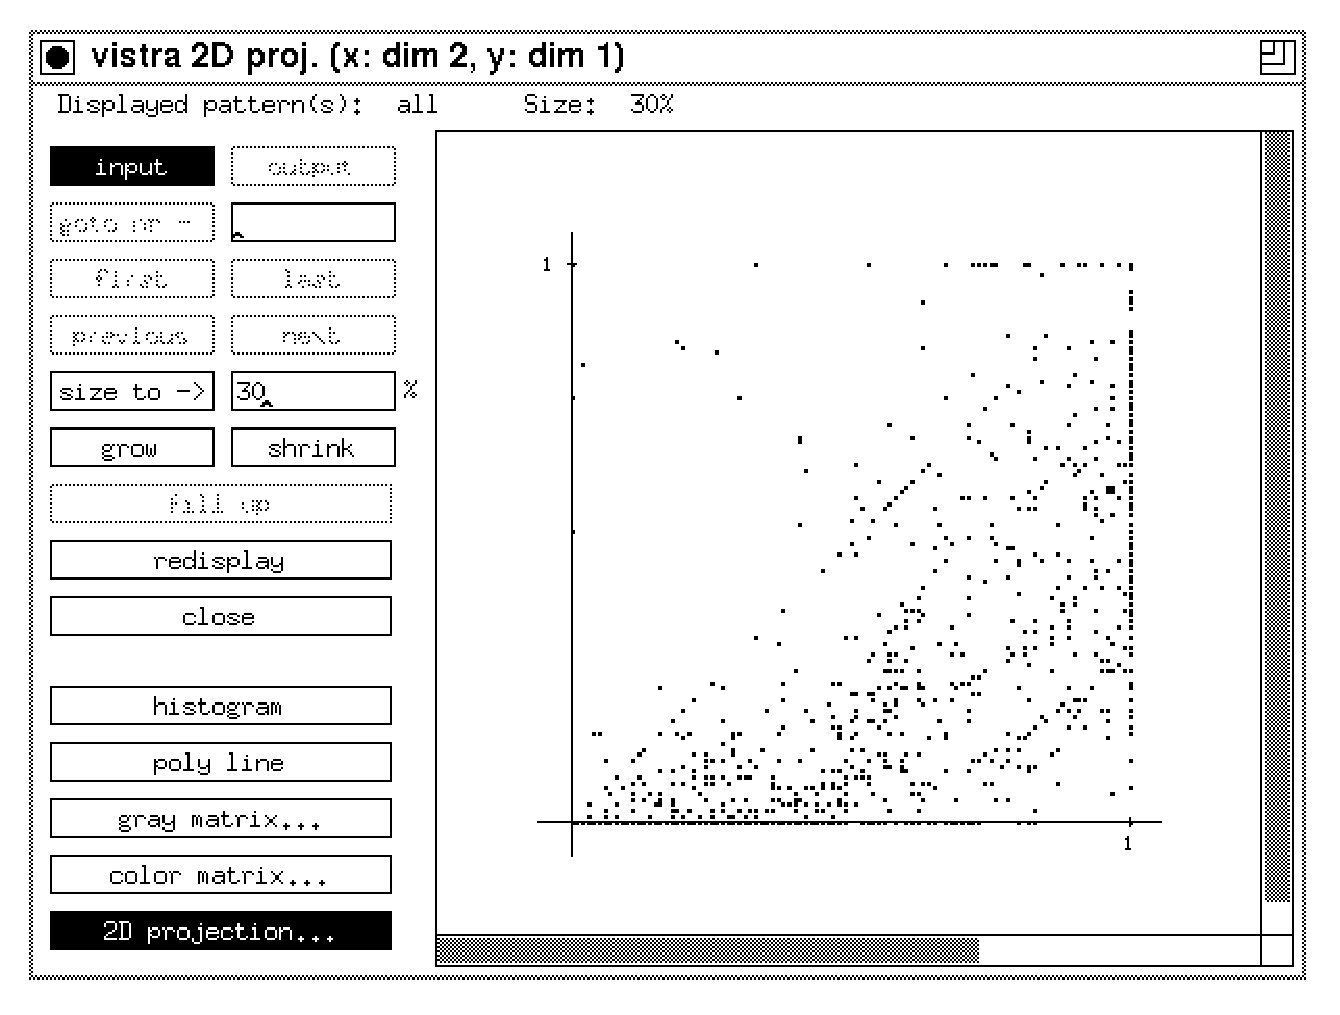
\psfig{file=proj2D.ps,width=\textwidth,height=10cm}}
\caption{\label{proj2D} Projektion zweier Dimensionen}
\end{figure}
 
\subsection{Das Statistik-Fenster}

Das Statistik-Fenster liefert allgemeine und statistische Informationen
"uber die geladenen Trainingsvektoren.
Abbildung~\ref{statistics} zeigt ein Beispiel.

\begin{figure}[ht]
\centerline{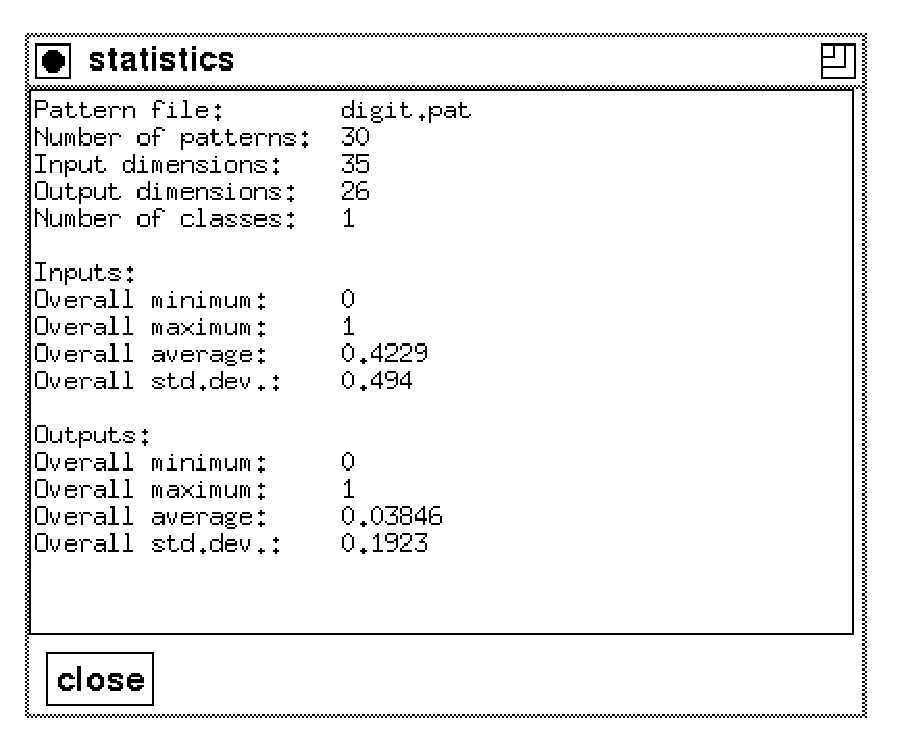
\psfig{file=stat.ps,width=10cm,height=8cm}}
\caption{\label{statistics} Das Statistik-Fenster}
\end{figure}

Der erste Teil zeigt allgemeine Informationen zu die Trainingsvektoren.
Die weiteren Abschnitte enthalten statistische Daten "uber 
die Eingabe- und Ausgabevektoren, wie sie auch "uber die "`Load"'-Men"us
des Hauptfensters berechnet werden k"onnen.  

Das Statistik-Fenster mu"s "uber "`close"' geschlossen werden, bevor
im Hauptfenster weitergearbeitet werden kann.

\subsection{Das Kovarianzmatrix-Fenster}

Das Kovarianzmatrix-Fenster zeigt eine Matrix, die alle Kovarianzen
zwischen je zwei Dimensionen der im Hauptfenster befindlichen Vektoren
enth"alt.
Stellt $nvecs$ die Anzahl der Vektoren und $ndims$ die Anzahl der
Dimensionen dar, so wird eine 
$ndims\times\/ndims$-Matrix $cov$ berechnet, in der das
Element $cov_{ij}$ die Kovarianz der Dimensionen $i$ und $j$ enth"alt. \\
Sei $avg_{i}$ der Mittelwert der Dimension $i$
($avg_{i} = \frac{1}{nvecs} \sum_{k=1}^{nvecs} v_{ki}$,  
$v_{k}$: $k$-ter Vektor), so berechnet sich $cov_{ij}$ wie folgt:

\[ cov_{ij} = \frac{1}{nvecs} \sum_{k=1}^{nvecs} 
(v_{ki} - avg_i)(v_{kj} - avg_j) 
\]    

F"ur $i=j$ erh"alt man aus obiger Formel:
\begin{displaymath}
cov_{ii} = \frac{1}{nvecs} \sum_{k=1}^{nvecs} 
(v_{ki} - avg_i)^{2}
\end{displaymath}
$cov_{ii}$ stellt also gerade die Varianz $\sigma^{2}_{i}$
der Dimension $i$ dar.
Die Matrix $cov$ ist au"serdem spiegelsymmetrisch, da f"ur alle $i,j$
gilt: $cov_{ij} = cov_{ji}$.

Abbildung~\ref{covariances} zeigt das Kovarianzmatrix-Fenster, das
die Kovarianzen f"ur folgende Vektoren enth"alt:

\nopagebreak
\begin{tabular}{l@{\hspace{1cm}}l}
{\sl Vektor~1:} & {\tt 0 2 1} \\
{\sl Vektor~2:} & {\tt 3 2 2} \\
{\sl Vektor~3:} & {\tt 1 2 3} \\
{\sl Vektor~4:} & {\tt 0 2 2} \\
\end{tabular}

\begin{figure}[ht]
\centerline{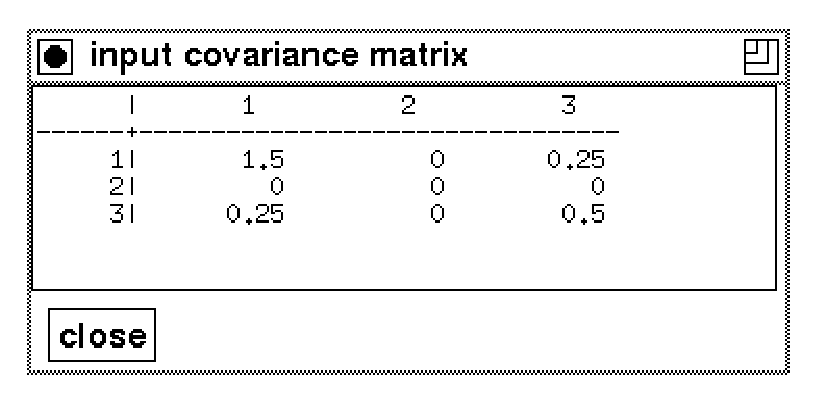
\psfig{file=cov.ps,width=8cm,height=4cm}}
\caption{\label{covariances} Das Kovarianzmatrix-Fenster}
\end{figure}

\subsection{Das Vektoren-Fenster}
\label{ssw}

Das Vektoren-Fenster kann nur ge"offnet werden, wenn Eingabe- und 
Ausgabevektoren vorhanden sind. 
Werden im Hauptfenster die Eingabevektoren (Ausgabevektoren) bearbeitet, 
so enth"alt das Vektoren-Fenster die Ausgabevektoren (Eingabevektoren).
Die Vektoren k"onnen im Vektoren-Fenster nur gelesen werden, 
Transformationen sind nur im Hauptfenster m"oglich.
Abbildung~\ref{vektorfenster} zeigt ein Vektoren-Fenster, in dem
momentan die Dimensionen 17 bis 22 der Vektoren 1 bis 22 angezeigt werden.
Der Titel des Fensters besagt, da"s es sich hierbei um die
Eingabevektoren handelt. 
"Uber den "`close"'-Button wird das Fenster wieder geschlossen. 

\begin{figure}[ht]
\centerline{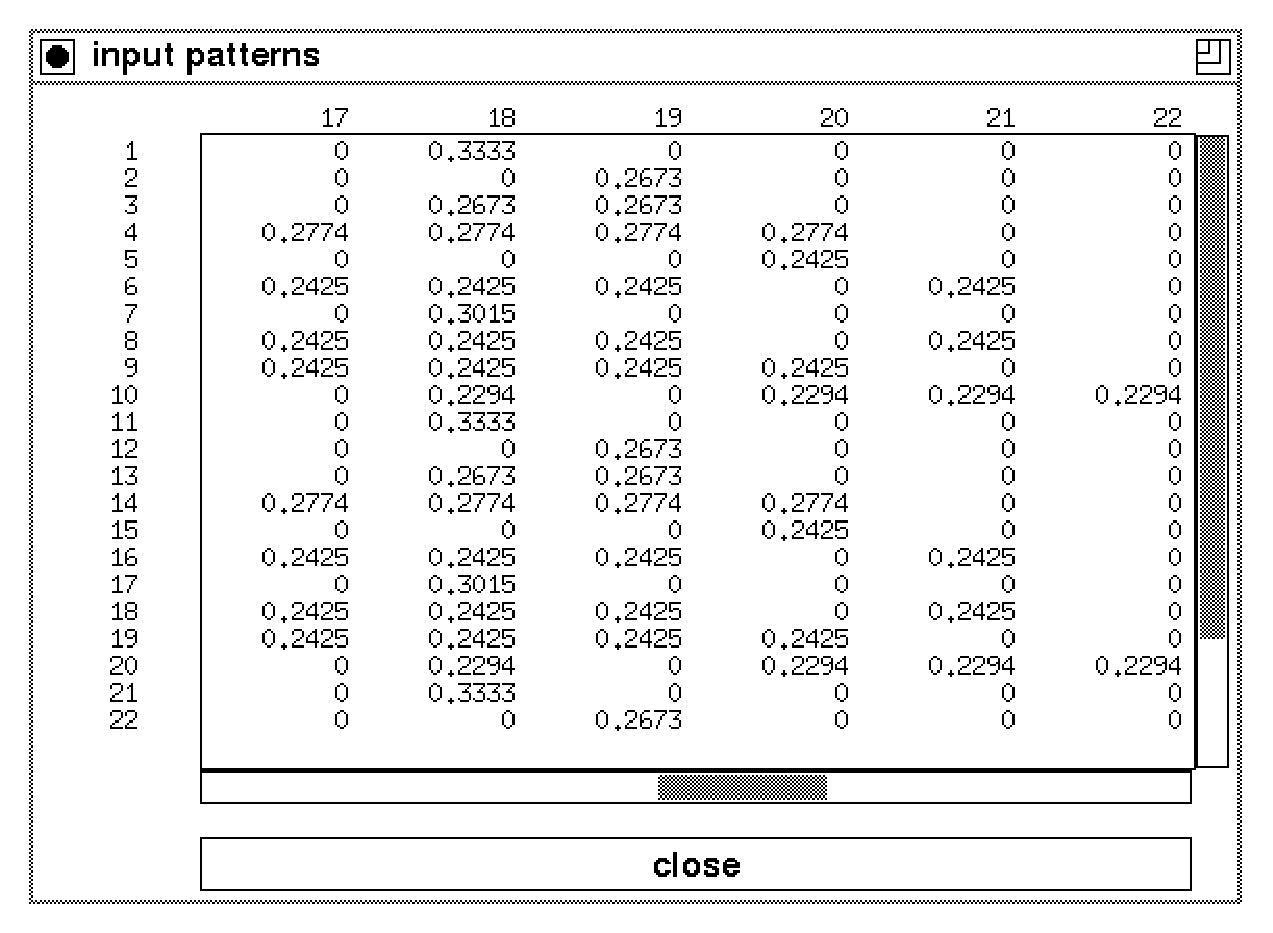
\psfig{file=readsh.ps,width=\textwidth,height=8cm}}
\caption{\label{vektorfenster} Das Vektoren-Fenster}
\end{figure}





%\section{Batch-Modus und LOG-Dateien}
\label{log}

Der Aufruf von Vistra im Batch-Modus wurde bereits in Abschnitt~\ref{call}
behandelt.
Dieses Kapitel beschreibt, wie LOG-Dateien zur Spezifikation eines 
durchzuf"uhrenden Jobs zu verwenden sind.

Eine LOG-Datei stellt eine Liste von Kommandos zur Transformation
von Trainingsvektoren dar.
Alle Transformationen, die interaktiv durchgef"uhrt werden, k"onnen 
mithilfe von LOG-Dateien auch im Stapelbetrieb durchgef"uhrt werden.
F"ur jede Transformation steht daf"ur ein entsprechendes Batch-Kommando
zur Verf"ugung.
Der Batch-Modus von Vistra erh"alt als Eingabe eine Trainingsvektor-Datei
und eine LOG-Datei, arbeitet die Befehle der LOG-Datei der Reihe nach
ab und schreibt die transformierten Trainingsvektoren wieder in eine
Ausgabe-Datei.  

Dem Batch-Modus fallen zwei Aufgaben zu:
\begin{itemize}
\item Transformationen k"onnen sowohl interaktiv "uber die X-Windows 
Oberfl"ache als auch als Job im Stapelbetrieb durchgef"uhrt werden.
Dazu ist eine LOG-Datei von Hand zu erstellen.
\item Der Batch-Modus erm"oglicht eine Trennung in
Trainings- und Testdaten oder ganz allgemein eine Aufteilung von
Trainingsvektoren in separate Dateien.
Die Transformationen, die interaktiv auf einen Satz der Trainingsvektoren 
angewandt werden, k"onnen in einer LOG-Datei festgehalten
werden, indem das Flag "`Write to log file"' des "`File"'-Men"us
gesetzt wird.
Sp"ater k"onnen die anderen Dateien durch Angabe dieser LOG-Datei 
im Batch-Modus auf die gleiche Weise umgewandelt werden.
\end{itemize}  
   
\subsection{Das Format von LOG-Dateien}

LOG-Dateien besitzen eine Zeilenstruktur.
Jede Zeile enth"alt eine Anweisung bzw. eine durchzuf"uhrende 
Transformation und besteht
aus ein oder mehreren W"ortern bzw. Zahlen, die
durch Blanks oder Tabulatoren getrennt sind.
Die Syntax einer Befehlszeile ist:

{\tt ('i'|'I'|'o'|'O') <command> [ <arg1> <arg2> ... ]}  

oder

{\tt \% <comment>}

Das erste Wort einer Zeile mu"s also immer ein einzelnes Zeichen sein.
Ein {\tt i} bzw. {\tt I} bedeutet, da"s die Anweisung auf die Eingabevektoren
anzuwenden ist, ein {\tt o} bzw. {\tt O}, da"s sie sich auf die
Ausgabevektoren bezieht. 
Generell wird in LOG-Dateien nicht zwischen Gro"s- und
Kleinschreibung unterschieden. \\  
{\tt \%} leitet eine Kommentarzeile ein. 
Alle Zeichen dieser Zeile werden von Vistra ignoriert.   

{\tt <command>} steht f"ur ein Schl"usselwort, das angibt, welche
Aktion bzw. Transformation durchzuf"uhren ist.

Manche Anweisungen ben"otigen zur genaueren Spezifikation einen oder
mehrere Parameter, die in obiger Syntax durch die Liste 
{\tt <arg1> <arg2> ...} repr"asentiert werden. 
Parameter k"onnen sowohl Strings als auch Zahlen sein.
 
F"ur jede Aktion, die im interaktiven Modus
Trainingsvektoren ver"andert, steht ein entsprechendes Batch-Kommando
zur Verf"ugung.
Neben Kommandos f"ur die Transformationen des "`Transform"'-Men"us und
des "`Remove"'-Men"us"' existieren auch f"ur das Laden der vertikalen
und horizontalen Skalarfelder (also f"ur jeden Men"upunkt des "`Load"'-Men"us)
sowie f"ur die Vektor--Skalar Operationen ("`add"', "`subtract"', "`multiply"',
"`divide"' und "`replace\ldots"') entsprechende Batch-Anweisungen.
W"ahrend eine LOG-Datei abgearbeitet wird, merkt sich Vistra neben den
aktuellen Werten der Trainingsvektoren auch die Inhalte der vertikalen
und horizontalen Skalarfelder zu den verschiedenen Zeitpunkten.

{\bf Beispiel:} \\
Mithilfe einer LOG-Datei sollen die Elemente der Trainingsvektoren auf
den Wertebereich [-1,1] skaliert werden.
Anschlie"send ist von jedem Vektorelement der statistische Mittelwert
der zugeh"origen Dimension abzuziehen. 
Zum Schlu"s soll noch eine Hauptachsentransformation (PCA) durchgef"uhrt
werden. 

\begin{samepage}
Diese Transformationen k"onnten im Batch-Modus durch folgende LOG-Datei
vollzogen werden:
\begin{verbatim}
i scale -1 1
% Mittelwerte der Dimensionen sollen 0 sein
i loadHoriz avg
i subtract horiz
% zum Schluss: Hauptachsentransformation
i pca
\end{verbatim}  
\end{samepage}
 
Tabelle~\ref{batchcommands} zeigt alle Batch-Anweisungen plus zugeh"orige
Parameter.

\begin{table}
\begin{tabular}{c|c|p{7.5cm}}
{\tt <command>} & {\tt <arg1> <arg2> ...} & {\bf Aktion} \\ \hline
{\tt pca} & & Hauptachsentransformation \\
{\tt fft} & & 1-dimensionale diskrete Fourier Trans\-for\-ma\-tion \\
{\tt hlog} & & halblogarithmische Transformation \\
{\tt scale} & {\it min\quad max} & skaliere aufs Intervall 
[{\it min}, {\it max}] \\
{\tt normalize} & & normalisiere auf L"ange 1 \\
{\tt randomize} & & mische die Vektoren willk"urlich \\
{\tt classExpand} & & erweitere mit Klassenvektor \\
{\tt outputExpand} & & erweitere mit Ausgabevektor \\
{\tt refreshClasses} & & berechne die Klassen aus den
Aus\-ga\-be\-vek\-toren \\
{\tt rmDimRange} & {\it from\quad to} & entferne die Dimensionen {\it from} 
bis {\it to} \\
{\tt rmConstDims} & & entferne alle konstanten Dimensionen \\
{\tt rmDims} & $dim_1 \ldots dim_n$ & entferne die Dimensionen 
$dim_1, \ldots, dim_n$ \\ 
{\tt loadVert} & {\it loadparams} & lade die vertikalen Skalarfelder 
je nach {\it loadparams} mit bestimmten Werten (siehe unten) \\
{\tt loadHoriz} & {\it loadparams} & lade die horizontalen Skalarfelder 
je nach {\it loadparams} mit bestimmen Werten (siehe unten) \\
{\tt add} & {\it direction} & addiere die vertikalen 
({\it direction} = {\tt vert})
bzw. die horizontalen ({\it direction} = {\tt horiz}) Skalare zu den 
zugeh"origen Vektoren bzw. Dimensionen \\
{\tt subtract} & {\it direction} & subtrahiere die vertikalen 
({\it direction} = {\tt vert}) bzw. die horizontalen 
({\it direction} = {\tt horiz}) 
Skalare von den zugeh"origen Vektoren bzw. Dimensionen \\
{\tt multiply} & {\it direction} & multipliziere die vertikalen 
({\it direction} = {\tt vert}) bzw. die horizontalen 
({\it direction} = {\tt horiz}) 
Skalare mit den zugeh"origen Vektoren bzw. Dimensionen \\
{\tt divide} & {\it direction} & dividiere die Vektoren 
({\it direction} = {\tt vert})
bzw. die Dimensionen ({\it direction} = {\tt horiz}) durch die zugeh"origen 
vertikalen bzw. horizontalen Skalare \\
{\tt replace} & {\it direction\quad nr} & ersetze den Vektor Nummer~{\it nr} 
({\it direction} = {\tt horiz}) bzw. die Dimension~{\it nr} 
({\it direction} = {\tt vert}) durch die horizontalen 
bzw. vertikalen Skalare \\
{\tt addConst} & {\it num} & addiere {\it num} zu jedem Vektorelement \\
{\tt subConst} & {\it num} & subtrahiere {\it num} von jedem Vektorelement \\
{\tt multConst} & {\it num} & multipliziere jedes Vektorelement mit 
{\it num} \\
{\tt divConst} & {\it num} & dividiere jedes Vektorelement durch {\it num} \\ 
\end{tabular}
\caption{\label{batchcommands} Die Batch-Anweisungen}
\end{table}
  
Durch die Batch-Anweisungen {\tt loadVert} und {\tt loadHoriz} k"onnen
die vertikalen bzw. horizontalen Skalarfelder mit Werten geladen werden.
Unter anderem stehen alle Funktionen zur Verf"ugung, die auch interaktiv "uber
das "`Load"'-Men"u aufgerufen werden k"onnen. 

{\it loadparams} aus Tabelle~\ref{batchcommands} kann folgende Werte
annehmen: 

\nopagebreak
\begin{tabular}{c|c}
{\it loadparams} & {\bf entspricht "`Load"'-Men"upunkt\ldots} \\ \hline
{\tt min} & "`minimum"' \\
{\tt max} & "`maximum"' \\
{\tt avg} & "`average"' \\
{\tt length} & "`length"' \\
{\tt sum} & "`sum"' \\
{\tt stddev} & "`standard deviation"' \\
{\tt pattern} {\it nr} & "`pattern\ldots"' \\
{\tt overallMin} & "`overall minimum"' \\
{\tt overallMax} & "`overall maximum"' \\
{\tt overallAvg} & "`overall average"' \\
{\tt overallStddev} & "`overall std dev"' \\
{\tt const} {\it number} & "`const\ldots"' \\
{\tt values} $val_1 \ldots val_n$ & --- \\
{\tt dim} \enspace $nr$ \enspace $value$ & --- \\  
\end{tabular} 

F"ur die Anweisung {\tt const} gibt {\it number} die zu ladende Konstante an.
Die Anweisung {\tt pattern} l"adt den Vektor Nummer {\it nr}
in die horizontalen Skalarfelder ({\tt <command> = loadHoriz})
bzw. die {\it nr}-te Dimension in die vertikalen Felder 
({\tt <command> = loadVert}). \\
Durch {\tt values} k"onnen die Werte, mit denen die vertikalen bzw.
horizontalen Skalarfelder geladen werden sollen, direkt angegeben werden.
Diese Werte wurden in obiger Tabelle mit $val_1 \ldots val_n$ bezeichnet.
$n$ mu"s dabei genau der Anzahl der betreffenden Skalarfelder
entsprechen. \\
Wie f"ur {\tt values} gibt es auch f"ur die Anweisung {\tt dim} keine
Entsprechung im "`Load"'-Men"u.
Mit {\tt dim} wird das $nr$-te vertikale ({\tt <command> = loadVert})
bzw. das $nr$-te horizontale Skalarfeld ({\tt <command> = loadHoriz})
auf den Wert $value$ gesetzt.
{\tt dim} entspricht im interaktiven Modus somit einer "Anderung 
eines Skalarfeldes von Hand.
F"ur jedes ge"anderte Feld wird eine {\tt dim}-Anweisung in die LOG-Datei
geschrieben.   
 
\subsubsection*{Fehlerbehandlung im Batch-Modus}

Trifft Vistra in der LOG-Datei auf eine Zeile mit fehlerhafter Syntax,
so wird eine Warnung auf stdout ausgegeben und mit der 
n"achsten Zeile fortgefahren.
Gleiches gilt f"ur Anweisungen, die aus anderen Gr"unden 
nicht ausgef"uhrt werden k"onnen.
Eine halblogarithmische Transformation ben"otigt beispielsweise Vektoren
mit einer quadratischen Anzahl von Dimensionen.
Ein weiteres Beispiel ist die {\tt loadVert values}-Anweisung, die
eine Warnung erzeugt, wenn die Anzahl der Werte nicht der Anzahl
der Trainingsvektoren entspricht. 

\subsection{LOG-Anweisungen der interaktiven Aktionen}

Dieser Abschnitt besch"aftigt sich mit der Frage, welche LOG-Anweisungen
f"ur die Aktionen, die interaktiv im Hauptfenster von Vistra 
durchgef"uhrt werden, in die LOG-Datei geschrieben werden, solange 
"`Write to log file"' gesetzt ist.
Dabei ist zu beachten, da"s eine Trennung von Trainingsvektoren nur
dann sinnvoll unterst"utzt wird, wenn ein und derselbe Vektor durch
Ausf"uhrung der LOG-Datei in genau der gleichen Weise ver"andert wird wie 
durch die interaktiv durchgef"uhrten Transformationen.

Vektor-Transformationen, deren Ergebnisse nur vom jeweiligen Vektor 
abh"angen, bereiten unter diesem Gesichtspunkt keine Probleme
(z.B. liefert eine Fourier Transformation auf den gleichen Vektor angewandt
immer das gleiche Resultat).
Schwierigkeiten machen jedoch Aktionen, die von {\it allen} geladenen
Vektoren abh"angen.
Darunter f"allt beispielsweise das Entfernen konstanter Dimensionen.
Eine Dimension, die f"ur eine Menge von Vektoren konstant ist, mu"s
nicht auch f"ur andere Vektormengen konstant sein.
W"urde in diesem Fall einfach nur {\tt rmConstDims} in die LOG-Datei
geschrieben, so k"onnten den Vektoren einer Datei evtl. ganz andere Dimensionen
entfernt werden als den Trainingsvektoren einer anderen Datei. 
Abhilfe kann nur geschaffen werden, wenn die LOG-Datei  
die tats"achlich entfernten Dimensionen explizit enth"alt (mithilfe
von {\tt rmDims}).      

"Ahnlich verh"alt es sich, wenn z.B. die horizontalen Skalarfelder 
mit den Minima der einzelnen Dimensionen geladen werden sollen.
Die Minima k"onnen je nach Vektormenge anders ausfallen, weshalb auch
hier anstelle von {\tt loadHoriz min} 
das Minimum jeder Dimension explizit in die LOG-Datei geschrieben wird.

Folgende Tabelle enth"alt in der linken Spalte die 
interaktiven Aktionen und in der rechten die daf"ur geschriebenen 
LOG-Anweisungen:

\begin{tabular}{l|l}
{\bf Men"upunkt/Button} & {\bf geschriebene LOG-Anweisung(en)} \\ \hline
"`HLOG"' & {\tt hlog} \\
"`FFT"' & {\tt fft} \\
"`PCA"' & {\tt pca} \\
"`Normalize"' & {\tt normalize} \\
"`Scale"' & {\tt multConst} {\it stretch} \\
& {\tt addConst} {\it shift} \\
"`Randomize"' & {\tt randomize} \\
"`Expand with class vector"' & {\tt classExpand} \\
"`Expand with output vector"' & {\tt outputExpand} \\
"`Refresh class numbers"' & {\tt refreshClasses} \\
"`Remove dimensions"' & {\tt rmDimRange} {\it from to} \\
"`Remove constant dims"' & {\tt rmDims} $dim_1 \ldots dim_n$ \\
"`add"' & {\tt add} {\it direction} \\
"`subtract"' & {\tt subtract} {\it direction} \\
"`multiply"' & {\tt multiply} {\it direction} \\
"`divide"' & {\tt divide} {\it direction} \\
"`replace"' & {\tt replace} {\it nr} \\
\end{tabular}

Eine Skalierung eines Wertebereichs auf einen anderen kann auf
eine Multiplikation und eine Addition zur"uckgef"uhrt werden.
Der betreffende Faktor bzw. Summand ist oben als {\it stretch} bzw.
{\it shift} bezeichnet. \\
{\it direction} steht entweder f"ur {\tt vert} oder f"ur {\tt horiz}.

In obiger Tabelle fehlen die Aktionen des "`Load"'-Men"us.
Bei ihnen h"angen die geschriebenen LOG-Anweisungen davon ab, ob die vertikalen
oder die horizontalen Skalarfelder geladen wurden:

\begin{tabular}{l|l|l}
{\bf "`Load"'-Men"upunkt} & {\bf vertikal} & {\bf horizontal} \\ \hline
"`minimum"' & {\tt loadVert min} & {\tt loadHoriz values} {\it valueList} \\
"`maximum"' & {\tt loadVert max} & {\tt loadHoriz values} {\it valueList} \\
"`average"' & {\tt loadVert avg} & {\tt loadHoriz values} {\it valueList} \\
"`length"' & {\tt loadVert length} & {\tt loadHoriz values} {\it valueList} \\
"`standard deviation"' & {\tt loadVert stddev} & {\tt loadHoriz values} 
{\it valueList} \\
"`sum"' & {\tt loadVert sum} & {\tt loadHoriz values} {\it valueList} \\
"`pattern"' & {\tt loadVert values} {\it valueList} &
{\tt loadHoriz values} {\it valueList} \\
"`overall minimum"' & {\tt loadVert const} {\it value} &
{\tt loadHoriz const} {\it value} \\   
"`overall maximum"' & {\tt loadVert const} {\it value} &
{\tt loadHoriz const} {\it value} \\   
"`overall average"' & {\tt loadVert const} {\it value} &
{\tt loadHoriz const} {\it value} \\   
"`overall std dev"' & {\tt loadVert const} {\it value} &
{\tt loadHoriz const} {\it value} \\   
"`const"' & {\tt loadVert const} {\it value} & 
{\tt loadHoriz const} {\it value} \\ 
\end{tabular}

{\it valueList} repr"asentiert hierbei eine Liste von Zahlen, die jeweils 
durch ein Blank voneinander getrennt sind.
Eine letzte M"oglichkeit zur Manipulation der Skalarfelder ist 
das direkte "Andern eines Feldinhalts von Hand mithilfe der Tastatur.
In diesem Fall wird einer der folgenden beiden Anweisungen in die
LOG-Datei geschrieben (je nachdem, ob es sich um ein vertikales oder
ein horizontales Skalarfeld handelt):

{\tt loadVert dim} \enspace $nr$ \enspace $value$ \qquad oder \\
{\tt loadHoriz dim} \enspace $nr$ \enspace $value$  

Das $nr$-te vertikale bzw. horizontale Skalarfeld wird hierdurch auf
den Wert $value$ gesetzt.
%\section{Datei-Formate}
\label{formate}

Dieses Kapitel beschreibt, welche Formate die LVQ-, N01- und 
Symboltabellen-Dateien haben bzw. haben
m"ussen, wenn sie von Vistra geschrieben bzw. gelesen werden
(siehe auch \cite{bayer}).
Das Format der LOG-Dateien wurde bereits in Kapitel~\ref{log} erl"autert.
Formatbeschreibungs-Dateien sind Thema des Kapitels~\ref{fdl}, 
in der die Syntax von FDL (Format Description Language) beschrieben
wird und einige Beispiele f"ur benutzerdefinierte ASCII-Dateiformate
gegeben werden.

\subsection{Das LVQ-Format}
\label{lvq}

Das LVQ-Format ist ein sehr einfaches Trainingsvektor-Format, das eine Menge von
Eingabevektoren enth"alt und jedem dieser Vektoren ein Klassensymbol
zuordnet.

Das LVQ-Format setzt sich aus einem Kopf und einem Rumpf zusammen.
Der Kopf besteht lediglich aus einer Zeile, die die Dimensionalit"at der
Eingabevektoren enth"alt.
Der Rumpf besitzt pro Eingabevektor eine Zeile, in der die Elemente
des jeweiligen Vektors gefolgt von seinem Klassensymbol aufgef"uhrt sind.

Folgendes Beispiel zeigt ein LVQ-File, das zweidimensionale
Trainingsvektoren enth"alt, die das xor-Problem definieren:

\nopagebreak
\begin{verbatim}
2
0 0 NULL
0 1 EINS
1.0 0.0 EINS
1 1.0 NULL
\end{verbatim}
   
\subsection{Das N01-Format}
\label{n01}
Das N01-Format ist ein bin"ares Format, das geschaffen wurde, um das
Einlesen bzw. Schreiben von Trainingsvektor-Dateien zu beschleunigen.
Bei sehr gro"sen Vektor-Dateien ist es daher empfehlenswert, 
anstelle eines ASCII-Formats dieses Format zu verwenden.

Die ersten 32 Bytes stellen den Kopf des N01-Formats dar.
Er hat folgende Gestalt:

\nopagebreak
\begin{tabular}[t]{l|l|l}
{\bf Bytes} & {\bf C-Typ} & {\bf Inhalt} \\ \hline
0~--~3 & char[4] & String ''N01'' mit abschlie"sender '$\backslash0$' \\
4~--~7 & unsigned int & Dimensionalit"at der Eingabevektoren \\
8~--~11 & unsigned int & Dimensionalit"at der Ausgabevektoren \\
12~--~15 & unsigned int & Anzahl der Trainingsvektoren \\
16~--~19 & unsigned int & Offset der Eingabedaten \\
20~--~23 & unsigned int & Offset der Ausgabedaten \\
24~--~27 & unsigned int & Offset der Klassennummern \\
28~--~31 & unsigned int & Anzahl unterschiedl.~Klassen 
\end{tabular}  

Die Offsets geben die File-Positionen innerhalb der N01-Datei an, an denen
die Eingabevektoren, Ausgabevektoren oder Klassennummern beginnen.
Die Eingabe- bzw. Ausgabevektoren sind als Felder von aufeinanderfolgenden
Flie"skommazahlen von jeweils 4 Bytes (C-Typ: {\tt float}) gespeichert.
In diesen Feldern erscheinen zun"achst alle Elemente des ersten 
Eingabe- bzw. Ausgabevektors, gefolgt von den Elementen des zweiten etc.
Die Klassennummern sind in einem Feld aufeinanderfolgender
Integer von jeweils 4 Bytes L"ange untergebracht (C-Typ: {\tt unsigned int}).
Die L"ange des Felds entspricht der Anzahl der Trainingsvektoren.

Das N01-Format wurde urspr"unglich f"ur DEC Workstations eingef"uhrt,
weshalb deren Maschinencodierung von {\tt float} bzw. {\tt unsigned} Typen
verwendet wird.
Hierbei erscheint das niederwertigste Byte als erstes,
das h"oherwertigste als letztes Byte innerhalb der Datei.

Vistra kann N01-Formate jedoch in jedem Fall lesen und schreiben
(unabh"angig davon, ob es auf einer SUN oder einer DEC l"auft).
Das Programm stellt fest, ob die Maschinencodierung des Rechners, auf dem
es l"auft, mit der DEC-Codierung "ubereinstimmt.
Ist dies nicht der Fall (wie bei den Maschinen der Marke SUN), so
werden alle Daten nach dem Einlesen bzw. vor dem Schreiben der N01-Datei
in geeigneter Weise konvertiert. 
    
\subsection{Das Format der Symboltabellen}
\label{symtab}

Symboltabellen-Dateien haben eine Zeilenstruktur.
Jede Zeile enth"alt genau ein Symbol, wobei 
die $i$-te Zeile der Datei das Klassensymbol zur Klassennummer $i$ enth"alt.

Abh"angig davon, ob die geladenen Trainingsvektoren explizite
Klassensymbole besitzen (die durch Strings repr"asentiert werden) oder nicht,
ist der Inhalt der einzelnen Zeilen verschieden.

Existieren explizite Klassensymbole, so werden diese als 
Zeileninhalte verwendet.
Wurde z.B.~ein LVQ-File wie das aus Kapitel~\ref{lvq} geladen, so existieren
solche Klassensymbole. \\ 
\begin{samepage} Die Symboltabellen-Datei s"ahe wie folgt aus:
\begin{verbatim}
NULL
EINS
\end{verbatim}
\end{samepage}

Existieren keine expliziten Klassensymbole, so werden die Ausgabevektoren
als solche betrachtet.
Identische Vektoren stellen dasselbe Klassensymbol dar.
Eine Zeile der Sym\-bol\-tabel\-len-Datei besteht dann gerade aus den Elementen
eines Ausgabevektors und die
Anzahl der Zeilen der Symboltabelle entspricht genau der Anzahl der
unterschiedlichen Ausgabevektoren.
Die Ausgabevektoren werden in der Reihenfolge ausgegeben, in der sie 
zum ersten Mal in den Trainingsvektoren auftauchen.

\begin{samepage}
Eine Symboltabelle f"ur Trainingsvektoren mit zweidimensionalen 
Ausgabevektoren, die keine expliziten Klassensymbole besitzen, k"onnte
wie folgt aussehen:
\begin{verbatim}
0.1 0.9
0.9 0.9
0.9 0.1
0.1 0.1
\end{verbatim}
\end{samepage}

%\section{Hinzuf"ugen neuer ASCII-Formate f"ur Vektordateien}
\label{fdl}

Vistra kann um benutzerdefinierte ASCII-Formate f"ur 
Trainingsvektor-Dateien erweitert werden.
Dazu sind folgende drei Schritte notwendig:

\begin{enumerate}
\item Erzeugen einer ASCII-Datei, die das neue Format in der 
Formatbeschreibungssprache FDL definiert.
Der Name dieser Datei mu"s auf {\tt .fmt} enden.
\item Kopieren der FDL-Datei in das Verzeichnis, das durch die 
Environment-Variable VISTRAFORMATS gegeben ist.
\item Neustarten von Vistra, um das neue Format einzubinden.
\end{enumerate}

\subsection{Die Formatbeschreibungssprache FDL}

Die Beschreibung eines Formats in FDL "ahnelt von der Struktur her 
einer Auspr"agung dieses Formats.

Der erste Unterschied besteht jedoch darin, da"s in der FDL-Beschreibung Angaben
"uber Dimensionen, die Anzahl der Vektoren etc. durch bestimmte
Steuersymbole, den sogenannten {\it Deskriptoren}, ersetzt werden.
Auch f"ur Klassensymbole, Eingabe- und Ausgabevektoren existieren
entsprechende Deskriptoren. \\ 
Der zweite Unterschied ist, da"s Wiederholungen (z.B.~eine Aufz"ahlung
aller Eingabevektoren) durch Schleifenkonstrukte dargestellt werden.

Zur Veranschaulichung soll eine FDL-Beschreibung des LVQ-Formats dienen.
Vistra be\-n"o\-tigt zwar keine FDL-Beschreibung dieses Standard-Formats, da
Lese- und Schreibroutinen festcodiert vorliegen.
Als einf"uhrendes Beispiel f"ur FDL ist sie jedoch sehr geeignet.   

\subsubsection*{Beispiel~1: FDL-Spezifikation des LVQ-Formats}
\begin{samepage} Eine FDL-Beschreibung des LVQ-Formats lautet:
\begin{verbatim}
%e <
{ %i %c < }
\end{verbatim}  
\end{samepage}
Die erste Zeile enth"alt zwei Deskriptoren.
{\tt \%e} gibt an, da"s an dieser Stelle die Dimensionalit"at der 
Eingabevektoren erscheint.
Der zweite Deskriptor {\tt <} bedeutet "`new-line"', d.h. "uberall wo
dieser Deskriptor auftaucht mu"s in der Vektor-Datei eine neue Zeile
beginnen.

Die zweite Zeile der obigen FDL-Beschreibung enth"alt eine 
{\it repetition}-Schleife.
Anfang bzw. Ende der Schleife sind durch {\tt \{} bzw. {\tt \}} markiert.
Der Rumpf besteht aus einer Liste von einem oder mehreren Deskriptoren,
in diesem Fall aus den Deskriptoren {\tt \%i}, {\tt \%c} und {\tt <}.  
Das {\it repetition}-Konstrukt repr"asentiert eine null- oder mehrmalige
Wiederholung der Deskriptoren innerhalb des Rumpfs.
Im Beispiel bedeutet dies, da"s in der Vektor-Datei zun"achst der
erste Eingabevektor gefolgt vom zugeh"origen Klassensymbol erscheint,
anschlie"send der zweite Eingabevektor mit zugeh"origem Klassensymbol
usw. 
Nach jedem Klassensymbol mu"s eine neue Zeile begonnen werden.

Neben Deskriptoren und {\it repetition}-Schleifen gibt es als letztes
FDL-Sprachmittel noch die sogenannten {\it matchOne}-Schleifen.
Eine {\it matchOne}-Schleife steht f"ur das null- oder mehrmalige
Ausw"ahlen einer Alternative.
Sie wird durch die Zeichen {\tt [} und {\tt ]} begrenzt und enth"alt im 
Rumpf eine oder mehrere Listen von Deskriptoren, die die
verschiedenen Alternativen darstellen und durch {\tt |} getrennt sind.
Die {\it matchOne}-Schleife wird verst"andlicher, wenn man sich ein
Beispiel ansieht.

\subsubsection*{Beispiel~2:}
Folgendes Format f"ur eine Vektor-Datei w"are denkbar:
\begin{itemize}
\item jede Zeile enth"alt einen Eingabevektor, einen Ausgabevektor oder
einfach einen Kommentar
\item eine Zeile, die einen Eingabevektor enth"alt, beginnt mit {\tt input:}
und wird gefolgt von den Vektorelementen
\item bei Ausgabevektoren beginnt die Zeile mit {\tt output:}
\item es spielt keine Rolle, ob zuerst die Eingabevektoren oder die
Ausgabevektoren erscheinen. 
Ein- und Ausgabevektoren d"urfen auch beliebig abwechseln.
\end{itemize}  
\begin{samepage}
Das Format w"urde in FDL wie folgt aussehen:
\begin{verbatim}
[ input:  %i < | 
  output: %o < | 
  * 
]
\end{verbatim}
\end{samepage}
Der {\tt *} ist ein Deskriptor, der f"ur einen beliebigen String bis
einschlie"slich dem
n"achsten {\it new-line}-Zeichen steht und im Beispiel~2 somit die
Kommentar-Zeilen repr"asentiert. \\
{\tt \%o} repr"asentiert einen Ausgabevektor. 

Folgende Vektor-Dateien des xor-Problems w"aren zul"assige
Auspr"agungen des Bei\-spiel-Formats~2:

\nopagebreak
\parbox[t]{6cm}{
{\sl Auspr"agung~1} \\[1ex]
{\tt Ausgabe-Muster \\
output: 0 \\
output: 1 \\
output: 1 \\
output: 0.0 \\ 
\\
Eingabe-Muster \\
input: 0.0 0.0 \\
input: 0 1 \\
input: 1.0 0 \\
und noch eins... \\
input: 1 1 }} 
\parbox[t]{6cm}{{\sl Auspr"agung~2} \\[1ex] 
{\tt die ersten 2 abwechselnd \\
input:   0  0 \\
output:  0 \\
input:   0  1 \\
output:  1 \\
die letzten 2 getrennt \\
input:   1  0 \\
input:   1  1 \\
output:  1 \\
output:  0 }
}

Bei der {\it matchOne}-Schleife ist zu beachten, da"s Vistra beim
Einlesen die Alternativen des Rumpfs in der Reihenfolge durchprobiert,
in der sie angegeben sind.
Ein {\tt *}, der eine Kommentarzeile repr"asentiert, sollte daher
stets die letzte Alternative darstellen, da dieser Deskriptor auf
jede Zeile der Vektordatei pa"st.
Im obigen Beispiel w"urden folglich auch die Zeilen mit den Vektoren
als Kommentarzeilen betrachtet und einfach "uberlesen werden.

\subsubsection*{Beispiel~3: das PAT-Format}

Als weiteres Beispiel dient ein Format, das vom SNNS (Stuttgarter
Neuronale Netze Simulator) der Universit"at Stuttgart f"ur die 
Trainingsvektoren verwendet wird. \\
Das PAT-Format kann textuell folgenderma"sen beschrieben werden:

\nopagebreak
\begin{itemize}
\item die Datei gliedert sich in einen Kopf und einen Rumpf
\item die ersten zwei Zeilen des Kopfs k"onnten wie folgt aussehen:
\begin{verbatim}
SNNS pattern definition file V1.4 
generated at Mon May 13 10:22:34 1993 
\end{verbatim}
Die erste Zeile enth"alt eine SNNS-Kennung plus Versionsnummer.
Die zweite Zeile gibt Datum und Uhrzeit an, zu der die Vektordatei
erzeugt wurde. 
\item Anschlie"send kann der Kopf folgende drei Muster enthalten:
\begin{itemize}
\item {\tt No. of patterns :} {\it numberOfPatterns}
\item {\tt No. of input units :} {\it inputDimension}
\item {\tt No. of output units :} {\it outputDimension}
\end{itemize} 
Dabei stehen die kursiv gedruckten W"orter f"ur Zahlen der 
entsprechenden Bedeutung.
\item der Rumpf besteht aus {\it numberOfPatterns} Bl"ocken der 
folgenden Form:
\begin{itemize}
\item ein Kommentar, der mit {\tt \#} beginnt
\item eine Zeile mit {\it inputDimension} Werten, die die Elemente
eines Eingabevektors darstellen 
\item eine Zeile mit {\it outputDimension} Werten, die die Elemente
des zugeh"origen Ausgabevektors darstellen 
\end{itemize}
\end{itemize}

Das xor-Problem k"onnte im PAT-Format wie folgt aussehen:

\nopagebreak
\begin{verbatim}
SNNS pattern definition file V1.4 
generated at Mon May 13 10:22:34 1993 

No. of patterns : 4
No. of input units : 2
No. of output units : 1
#1
0 0
0
#2
0 1
1
#3
1.0 0.0
1.0
#4
1 1
0
\end{verbatim}

Folgende Beschreibung in FDL w"are m"oglich:

\nopagebreak
\begin{verbatim}
SNNS pattern definition file V1.4 * 
generated at * \
[ No. of patterns : %n \ |
  No. of input units : %e \ |
  No. of output units : %a \ |
  *
]
{ #* 
  %i %o <
}
\end{verbatim}

Obige Beschreibung l"a"st durch den Deskriptor {\tt *} zu, da"s hinter
der Versionsnummer in der ersten Zeile noch weitere Zeichen stehen d"urfen.
Der {\tt *} in der zweiten Zeile ersetzt das Datum und die Uhrzeit.
Dabei wurde der Umstand ausgen"utzt, da"s der SNNS die Uhrzeit 
beim Einlesen von PAT-Dateien einfach ignoriert.
Eine Vektordatei, die durch Vistra mithilfe der obigen FDL-Spezifikation
geschrieben wird, kann aus diesem Grund auch ohne Zeitangabe vom SNNS
korrekt eingelesen werden.  

Desweiteren enth"alt obige FDL-Beschreibung von PAT zwei Deskriptoren, die
noch nicht erl"autert wurden.
{\tt \%n} repr"asentiert eine ganze Zahl $\geq 1$, die die Anzahl der 
Trainingsvektoren angibt, die in der Vektor-Datei enthalten sind.

Zur Erl"auterung des Deskriptors {\tt $\backslash$}, 
mu"s man mehr
"uber die Verwendung der FDL-Be\-schreib\-ungen durch Vistra wissen. \\
Vistra benutzt die FDL-Spezifikationen von Formaten sowohl zum Lesen
als auch zum Schreiben von Vektor-Dateien im betreffenden Format.
Dabei wird jeder Deskriptor bzw. jede Schleife als Anweisung f"ur
einen Interpreter betrachtet.
Es existiert jeweils ein Interpreter f"ur das Schreiben und f"ur das Lesen.
Je nach Deskriptor f"uhren die Interpreter unterschiedliche Aktionen 
auf der zu lesenden bzw. zu schreibenden Vektor-Datei aus.

Der Deskriptor {\tt $\backslash$} wird beim Lesen von Vektor-Dateien ignoriert.
Er stellt lediglich beim Schreiben eine Anweisung f"ur den Interpreter
dar.
Sie lautet: "`beginne eine neue Zeile"'.
Der Deskriptor {\tt <} hat beim Schreiben einer Datei genau die gleiche
Wirkung, im Gegensatz zu {\tt $\backslash$} jedoch auch beim Lesen 
eine Bedeutung, 
die wie folgt lautet: "`teste, ob das n"achste Wort in einer neuen Zeile
beginnt; falls nicht, erzeuge einen Fehler"'.

\subsection{Die Syntax von FDL}

Die Syntax von FDL kann in BNF-Notation wie folgt beschrieben werden:

\begin{tabular}[t]{lll}
{\it fdl\_description} & ::= & {\it stmt\_list} \\
{\it stmt\_list} & ::= & {\it fdl\_stmt stmt\_list} $|$ {\it fdl\_stmt} \\
{\it fdl\_stmt} & ::= & {\it descriptor\_list $|$ matchOne\_loop $|$
repetition\_loop} \\
{\it repetition\_loop} & ::= & {\bf '\{'} {\it descriptor\_list} {\bf '\}'} \\
{\it matchOne\_loop} & ::= & {\bf '['} {\it alternatives} {\bf ']'} \\
{\it alternatives} & ::= & {\it descriptor\_list} {\bf '$|$'} 
            {\it alternatives} $|$ {\it descriptor\_list} \\
{\it descriptor\_list} & ::= & {\it descriptor descriptor\_list} $|$
            {\it descriptor} \\
{\it descriptor} & ::= & {\it any\_string} $|$ {\bf '?'} $|$ {\bf '*'} $|$
            {\bf '$<$'} $|$ {\bf '$\backslash$'} $|$ \\ 
& &         {\bf '\%e'} $|$ {\bf '\%E'} $|$ {\bf '\%a'} $|$ {\bf '\%A'} $|$ \\
& &         {\bf '\%i'} $|$ {\bf '\%I'} $|$ {\bf '\%o'} $|$ {\bf '\%O'} $|$ \\
& &         {\bf '\%c'} $|$ {\bf '\%C'} $|$ {\bf '\%n'} $|$ {\bf '\%N'}
\end{tabular}
       
Die Terminale dieser Grammatik sind fettgedruckt.
Um sie besser von den Nichtterminalen in obiger Grammatik zu unterscheiden,
wurden sie zus"atzlich in einfache Anf"uhrungszeichen eingeschlossen, die
jedoch in einer FDL-Beschreibung wegzulassen sind.

\begin{sloppypar}
Eine FDL-Beschreibung besteht aus einer Liste von Deskriptoren, 
{\it repetition-} und {\it matchOne-}Schleifen, wobei die Schleifen
nicht geschachtelt werden d"urfen.
Die Terminale der Grammatik k"onnen durch null oder mehrere Blanks, 
Tabulatoren oder Newlines getrennt sein.
\end{sloppypar}

Das Nichtterminal {\it any\_string} steht f"ur einen beliebigen String,
der kein Terminal enth"alt.
Soll ein String ein Zeichen enthalten, das ein Terminal der Grammatik
ist, so mu"s diesem ein {\tt \%}-Zeichen vorangestellt werden, damit es nicht
als Grammatik-Symbol fehlinterpretiert wird.

\begin{samepage} Hier die Liste aller Zeichenkombinationen, 
die die Terminale der Grammatik als einfaches Textzeichen repr"asentieren:
\begin{verbatim}
%{ = {   %} = }   %[ = [   %| = |   %] = ] 
%? = ?   %* = *   %< = <   %\ = \   %% = % 
\end{verbatim}    
\end{samepage}

\subsection{Zusammenfassung der Deskriptoren}

Tabelle~\ref{descriptors} enth"alt eine vollst"andige Liste aller 
FDL-Deskriptoren.

\begin{table}[thb]
\begin{tabular}{l|p{5.8cm}|p{5.8cm}}
{\bf Deskriptor} & {\bf steht f"ur\ldots} & {\bf geschrieben wird\ldots} \\
\hline
{\it any\_string} & {\it any\_string} & {\it any\_string} \\
{\tt ?} & ein beliebiges Wort &
'? ' \\
{\tt *} & alle Zeichen bis einschlie"slich dem n"achsten Zeilenende & 
'$\backslash$n' \\
{\tt <} & ein Zeilenende & '$\backslash$n' \\
{\tt $\backslash$} & --- (der Deskriptor {\tt $\backslash$} wird beim
Einlesen ignoriert und hat nur f"ur das Schreiben von 
Trai\-nings\-vek\-tor-Dateien eine Bedeutung) & '$\backslash$n' \\
{\tt \%e}, {\tt \%E} & eine ganze Zahl $\geq 1$, die die Dimensionalit"at der
Ein\-gabe\-vek\-toren spezifiziert & die Dimensionalit"at der 
Ein\-gabe\-vektoren \\
{\tt \%a}, {\tt \%A} & eine ganze Zahl $\geq 0$, die die Dimensionalit"at der
Ausgabevektoren spezifiziert. 0 bedeutet, da"s keine Ausgabevektoren
existieren. & die Dimensionalit"at der Ausgabevektoren oder '0', falls 
keine vorhanden \\
{\tt \%i}, {\tt \%I} & einen Eingabevektor. Die Vektorelemente m"ussen durch
ein oder mehrere Newlines, Tabulatoren oder Blanks getrennt sein. 
& ein Eingabevektor \\
{\tt \%o}, {\tt \%O} & einen Ausgabevektor. Die Vektorelemente m"ussen durch
ein oder mehrere Newlines, Tabulatoren oder Blanks getrennt sein.
  & ein Ausgabevektor, falls einer 
existiert, sonst eine Klassennummer. \\
{\tt \%c}, {\tt \%C} & ein Wort, das ein Klassensymbol darstellt. &
ein Klassensymbol, falls eines existiert, sonst eine Klassennummer. \\
{\tt \%n}, {\tt \%N} & eine ganze Zahl $\geq 1$, die die 
Anzahl der Trainingsvektoren
spezifiziert. & die Anzahl der Trainingsvektoren     
\end{tabular}  
\caption{\label{descriptors} Die FDL-Deskriptoren}
\end{table}

Die zweite Spalte der Tabelle gibt an, was durch die jeweiligen Deskriptoren
repr"asentiert wird.
Trifft der Interpreter beim Einlesen einer Trainingsvektor-Datei auf
einen Deskriptor, so wird "uberpr"uft, ob die dem aktuellen Dateizeiger 
folgenden Zeichen der Vektor-Datei zum Deskriptor passen oder nicht.
Passen sie, werden diese Zeichen eingelesen und in
internen Programmvariablen gespeichert (f"ur {\tt \%n} wird z.B. eine
positive ganze Zahl eingelesen, die die Anzahl der Trainingsvektoren
spezifiziert und die die weiteren Aktionen des Interpreters beeinflu"st)
oder die Zeichen werden einfach "uberlesen (z.B. bei {\tt *}).   
Pa"st der Inhalt der Vektor-Datei nicht zum Deskriptor, so wird
eine Fehlermeldung generiert, die die darauf hinweist, da"s die einzulesende
Vektor-Datei ein falsches Format besitzt und die Trainingsvektoren
nicht eingelesen werden k"onnen.

Die dritte Spalte beschreibt, was beim Schreiben einer Trainingsvektor-Datei
anstelle eines Deskriptors ausgegeben wird.

Die beiden n"achsten Abschnitte stellen die Vorgehensweise der
FDL-Interpreter beim Lesen bzw. Schreiben von Trainingsvektor-Dateien
detailliert dar. 

\newpage
\subsection{Der Lese-Interpreter}

Wie bereits erw"ahnt, besteht eine FDL-Beschreibung aus einer 
Folge von {\it Deskriptoren, repetition-}Schleifen und 
{\it matchOne-}Schleifen.
Diese FDL-Konstrukte sind als Anweisungen f"ur einen Interpreter 
zu verstehen, der das Einlesen von Trainingsvektor-Dateien 
steuert, die in einem benutzerdefinierten Format vorliegen. 
Abbildung~\ref{lesen} zeigt ein Programmschema, das die Arbeitsweise 
des Lese-Interpreters vereinfacht darstellt. 

\begin{figure}[ht]
\centerline{\fbox{\parbox{15cm}{
{\bf for each} $fdl\_stmt$ {\bf do} \\
\hspace*{0.5cm} {\bf switch(}$fdl\_stmt${\bf )} \\
\hspace*{1cm} $fdl\_stmt = desc$: \\
\hspace*{2cm} {\bf if} Deskriptor $desc$ pa"st auf den 
Vektordatei-Inhalt {\bf then} \\ 
\hspace*{2.5cm} lese alle Zeichen ein, die durch den Deskriptor abgedeckt 
werden \\
\hspace*{3cm} (siehe Spalte~2 der Tabelle~\ref{descriptors}); \\
\hspace*{2.5cm} speichere dabei gelesene Vektoren, Dimensionsangaben etc.; \\
\hspace*{2.5cm} "uberpr"ufe die Konsistenz der Angaben und erzeuge ggf. \\
\hspace*{3cm} eine Fehlermeldung; \\
\hspace*{2cm} {\bf else} Fehler \\
\hspace*{1cm} $fdl\_stmt = \{\ desc_{1}\ desc_{2}\ \ldots\ desc_{n}\ \}$: \\ 
\hspace*{2cm} $exitLoop$ := FALSE; \\
\hspace*{2cm} {\bf while not} $exitLoop$ {\bf do} \\
\hspace*{2.5cm} {\bf if} $desc_{1}$ pa"st auf den Vektordatei-Inhalt
{\bf then} \\ 
\hspace*{3cm} lese $desc_{1}, \ldots , desc_{n}$ ein; \\
\hspace*{3cm} {\bf if} alle Vektoren, Dimensionsangaben oder Klassen 
eingelesen {\bf then} \\
\hspace*{3.5cm} $exitLoop$ := TRUE; \\  
\hspace*{2.5cm} {\bf else} $exitLoop$ := TRUE; \\
\hspace*{2cm} {\bf endwhile} \\ 
\hspace*{1cm} $fdl\_stmt = [\ alt_{1}\ |\ alt_{2}\ |\ \ldots\ |\ alt_{n}\ ]$: \\ 
\hspace*{2cm} {\bf while} der erste Deskriptor hinter der Schleife 
(also nach '$]$') nicht \\
\hspace*{2cm} zum Vektordatei-Inhalt pa"st {\bf do} \\
%\hspace*{2.5cm} $altMatched$ := FALSE; \\
%\hspace*{2.5cm} $i$ := 1; \\
%\hspace*{2.5cm} {\bf while not} $altMatched$ {\bf and} $i \leq n$ {\bf do} \\
\hspace*{2.5cm} vergleiche zuerst $alt_1$, dann $alt_2$ etc. mit dem 
Vektordatei-Inhalt; \\ 
\hspace*{2.5cm} lese erste Deskriptor-Liste $alt_i$ ein, die pa"st; \\ 
\hspace*{2.5cm} {\bf if} keine Alternative pa"st {\bf then} Fehler; \\
\hspace*{2cm} {\bf endwhile} \\ 
\hspace*{0.5cm} {\bf endswitch} \\    
{\bf endfor} \\
"uberpr"ufe, ob \\
\hspace*{0.5cm} -- die Vektor-Datei vollst"andig gelesen wurde \\
\hspace*{0.5cm} -- mindestens ein Eingabevektor gelesen wurde \\
\hspace*{0.5cm} -- die Angabe "uber die Anzahl der Trainingsvektoren (\%n) mit
der \\
\hspace*{1cm} Anzahl gelesener Eingabevektoren "ubereinstimmt \\
\hspace*{0.5cm} -- Klassensymbole oder Ausgabevektoren gelesen wurden \\
\hspace*{0.5cm} -- die Anzahl gelesener Klassensymbole bzw. Ausgabevektoren
mit der Anzahl von \\ 
\hspace*{1cm} Eingabevektoren "ubereinstimmt 
(sofern Klassen bzw. Ausgabevektoren vorhanden) \\
Trifft einer dieser Punkte nicht zu, so erzeuge einen Fehler 
}}}
\caption{\label{lesen} Die Arbeitsweise des Lese-Interpreters}
\end{figure}

Konsistenzpr"ufungen finden nicht nur zum Schlu"s statt, sondern 
auch w"ahrend des Interpretierens von Deskriptoren, die mit {\tt \%} beginnen.
Diese Deskriptoren repr"asentieren Daten, die von Vistra intern gespeichert
werden.
Wird eine Konsistenzbedingung verletzt, so wird der Lesevorgang abgebrochen
und eine Fehlermeldung erzeugt, die die Art der Konsistenzverletzung
spezifiziert und die Zeile in der Trainingsvektor-Datei angibt, in der
der Fehler festgestellt wurde. 

Beim Interpretieren von {\tt \%e} bzw. {\tt \%a} wird "uberpr"uft, ob die
Angaben "uber die Dimensionalit"at der Eingabevektoren bzw. der Ausgabevektoren
mit fr"uher gelesenen Werten f"ur {\tt \%e} bzw. {\tt \%a} "ubereinstimmen.
Au"serdem werden die Angaben auch noch mit der Dimensionalit"at bereits
gelesener Eingabe- bzw. Ausgabevektoren verglichen.

Wird "uber {\tt \%n} die Anzahl der Trainingsvektoren eingelesen, so
wird dieser Wert mit evtl. vorher gemachten Angaben verglichen.
Au"serdem wird sichergestellt, da"s die Anzahl bisher gelesener 
Vektoren oder Klassen diesen Wert nicht "ubersteigt.

Beim Einlesen von Vektoren "uber die Deskriptoren {\tt \%i} oder {\tt \%o}
sind zwei F"alle zu unterscheiden.
Ist die Dimensionalit"at $d$ der Vektoren bereits bekannt (weil 
bereits ein entsprechender Vektor gelesen wurde oder bereits eine
{\tt \%e}- bzw. {\tt \%a}-Angabe gemacht wurde), so werden die n"achsten $d$
durch Whitespace getrennte Zahlen gelesen.
Ist die Dimensionalit"at unbekannt, so werden alle aufeinanderfolgenden
Zahlen der Vektor-Datei gelesen bis eine Zeichenfolge angetroffen wird,
die keine Zahl darstellt.  

%\newpage
\subsection{Der Schreib-Interpreter} 

Wie f"ur das Einlesen existiert auch f"ur das Schreiben von Trainingsvektoren
ein FDL-Interpreter.

Sehr einfach beschrieben, arbeitet der Interpreter wie folgt:

\nopagebreak
\begin{itemize}
\item F"ur einen {\it Deskriptor} wird eine Folge von Zeichen in die
Ausgabedatei geschrieben (siehe dritte Spalte der Tabelle~\ref{descriptors}).
\item Eine {\it repetition-}Schleife wird solange wiederholt, bis
kein Deskriptor des Schleifenrumpfs neue Daten mehr liefert.
Unter neuen Daten sind dabei bisher noch nicht geschriebene Eingabevektoren
({\tt \%i}), Ausgabevektoren ({\tt \%o}) oder Klassen ({\tt \%c}) zu verstehen 
bzw. bisher noch nicht 
geschriebene Angaben "uber die Anzahl von Trainingsvektoren ({\tt \%n}),
Eingabe-Dimensionen ({\tt \%e}) oder Ausgabe-Dimensionen ({\tt \%a}). 
\item Eine {\it matchOne-}Schleife wird solange wiederholt, 
bis in einem Schleifendurchlauf keine Alternative mehr geschrieben wurde.
Dabei werden die Alternativen (Deskriptor-Listen) in der Reihenfolge, in 
der sie aufgef"uhrt sind, geschrieben, sofern sie neue Daten liefern.       
\end{itemize}

Abbildung~\ref{schreiben} enth"alt eine vereinfachte Darstellung der
Arbeitsweise des Schreib-Inter\-pre\-ters in Form eines Programmschemas.

\begin{figure}[ht]
\centerline{\fbox{\parbox{15cm}{
{\bf for each} $fdl\_stmt$ {\bf do} \\
\hspace*{0.5cm} {\bf switch(}$fdl\_stmt${\bf )} \\
\hspace*{1cm} $fdl\_stmt = desc$: \\
\hspace*{2cm} schreibe Deskriptor $desc$ gem"a"s Spalte~3 der
Tabelle~\ref{descriptors}; \\
\hspace*{1cm} $fdl\_stmt = \{ desc_{1}\ desc_{2}\ \ldots\ desc_{n}\ \}$: \\
\hspace*{2cm} {\bf while} Liste $desc_{1} \ldots desc_{n}$ neue Daten
liefert {\bf do} \\
\hspace*{2.5cm} schreibe $desc_{1} \ldots desc_{n}$ gem"a"s Spalte~3 der
Tabelle~\ref{descriptors}; \\
\hspace*{2cm} {\bf endwhile} \\ 
\hspace*{1cm} $fdl\_stmt = [\ alt_{1}\ |\ alt_{2}\ |\ \ldots\ |\ alt_{n}\ ]$: \\ 
\hspace*{2cm} {\bf do} \\
\hspace*{2.5cm} $descriptor\_written =$ FALSE; \\
\hspace*{2.5cm} {\bf for} $alt := alt_{1}$ {\bf to} $alt_{n}$ {\bf do} \\
\hspace*{3cm} {\bf if} $alt$ liefert neue Daten {\bf then} \\
\hspace*{3.5cm} schreibe die Deskriptoren von $alt$ gem"a"s Spalte~3 der
Tabelle~\ref{descriptors}; \\
\hspace*{3.5cm} $descriptor\_written$ := TRUE; \\
\hspace*{3cm} {\bf endif} \\ 
\hspace*{2.5cm} {\bf endfor} \\
\hspace*{2cm} {\bf while} $descriptor\_written$ = TRUE; \\
\hspace*{0.5cm} {\bf endswitch} \\    
{\bf endfor} \\
"Uberpr"ufe, ob alle Eingabevektoren, Ausgabevektoren und Klassen geschrieben
wurden; \\
gebe ggf. eine entsprechende Warnung aus \\
}}}
\caption{\label{schreiben} Die Arbeitsweise des Schreib-Interpreters}
\end{figure}






%\newpage
\begin{thebibliography}{Bronstein 85}
\bibitem[Bayer 93]{bayer} H.~Bayer: {\it KPack (Version 3.1)
Benutzerhandbuch}, 1993.
\bibitem[Bronstein 85]{bronstein}
I.~N.~Bronstein, K.~A.~Semendjajew: {\it Taschenbuch der Mathematik};
Verlag Harri Deutsch, Thun und Frankfurt/Main, 1985.
\bibitem[Hertz 91]{hertz}
J.~Hertz, A.~Krogh, R.~G.~Palmer: {\it Introduction to the Theory
of Neural Computation}; Addison-Wesley, 1991.
\bibitem[J"ahne 91]{jaehne} 
B.~J"ahne: {\it Digitale Bildverarbeitung}; Springer-Verlag, Berlin, 1991.
\bibitem[Zell et al.~93]{zell}
A.~Zell et al.: {\it SNNS User Manual, Version 3.0}; 
Institut f"ur Parallele und Verteilte H"ochstleistungsrechner, 
Universit"at Stuttgart, 1993.
\end{thebibliography}
\addcontentsline{toc}{section}{Literatur}



\clearpage \section{Einf"uhrung}
\label{einf}

%Neuronale Netze stellen eine Alternative zu "`klassischen"' symbolischen
%oder numerischen Verfahren dar, die f"ur geeignete Aufgabenstellungen
%einfachere und bessere Ergebnisse liefern kann.
%Einsatzbereiche sind z.B. die Mustererkennung oder das Verstehen und
%Verarbeiten von Bildern.
%Charakteristisch f"ur neuronale Netze ist, da"s die L"osung eines Problems
%nicht {\sl programmiert}, sondern anhand von Daten {\sl gelernt} wird.

%Jedes neuronale Netz besteht aus einer Menge von Neuronen bzw. Zellen,
%die untereinander durch ein gewichtetes Netzwerk verbunden sind.
%Jedes Neuron nimmt dabei zu jedem Zeitpunkt einen bestimmten 
%Aktivierungszustand an und besitzt einen Ausgabewert, der sich aus
%dem Aktivierungszustand durch Anwendung einer zum Neuron geh"orenden
%Ausgabefunktion berechnet. 

%Neuronen k"onnen in Eingabezellen, Ausgabezellen und "`versteckte"'
%Zellen eingeteilt werden.  
%Das neuronale Netz wird {\sl trainiert}, indem Eingabemuster 
%an die Eingabezellen
%angelegt werden (d.h. die Aktivierungen der Eingabezellen gesetzt werden)
%und in mehreren Schritten die Aktivierungen aller Zellen aus 
%den Ausgabewerten ihrer Vorg"anger sowie der 
%Gewichte der zugeh"origen Verbindungen neu berechnet werden.
%Anschlie"send werden die Werte der Ausgabezellen mit den gew"unschten
%Werten verglichen und die Gewichte der Verbindungen gem"a"s einer
%Lernregel in Abh"angigkeit von den beobachteten Abweichungen modifiziert.
%Das neuronale Netz {\sl lernt}.

Aufgabe der Studienarbeit war der Entwurf und die Implementierung eines
Programms, mit dem Eingabe- und Ausgabemuster f"ur neuronale Netze
transformiert und visualisiert werden k"onnen.
Als Eingabemuster ist hierbei ein Vektor zu verstehen, dessen Elemente
die Aktivierungen der Eingabezellen des neuronalen Netzes repr"asentieren.
Analog ist ein Ausgabemuster ein Vektor der Ausgabewerte der 
Ausgabezellen.
Trainings- bzw. Testdaten eines Netzes sind also
eine Menge von Eingabevektoren mit den zugeh"origen Ausgabevektoren.
Zur Spezifikation der Ausgabe werden zus"atzlich zu oder anstelle von den
Ausgabevektoren Klassen eingesetzt, die durch Nummern oder Klassensymbole
repr"asentiert werden.

Bevor Trainings- oder Testdaten in einem Simulator f"ur neuronale
Netze (wie z.B. KNet oder SNNS -- Stuttgarter Neuronale Netze Simulator --
der Universit"at Stuttgart) benutzt werden, ist es h"aufig w"unschenswert,
sich die Daten zun"achst graphisch oder textuell anzusehen und 
ggf.~einen oder mehrere Vorverarbeitungsschritte auf sie anzuwenden.
Desweiteren ben"otigen Simulatoren f"ur neuronale Netze zum Teil
sehr unterschiedliche Dateiformate f"ur die einzulesenden bzw.
zu schreibenden Trainingsvektoren.

Im Rahmen dieser Studienarbeit wurde das Programm "`Vistra"' entwickelt, das
\begin{itemize}
\item Trainingsdaten unterschiedlicher Formate lesen und schreiben
kann (Konvertierungsfunktion),
\item Trainingsdaten textuell und graphisch darstellen kann
(Visualisierungsfunktion),
\item Trainingsdaten transformieren und statistisch
auswerten kann (Manipulationsfunktion) sowie
\item um neue ASCII-Formate f"ur Trainingsvektor-Dateien erweitert werden 
kann mittels Vistra's Format-Beschreibungssprache FDL.
\end{itemize}
Durch die Konvertierungsfunktion ist Vistra vollkommen unabh"angig 
vom verwendeten Simulator f"ur neuronale Netze. 
Das Programm kann ganz allgemein zur Visualisierung und Manipulation von
Trainingsvektoren verwendet werden.

Auch eine Trennung von Trainings- und Testdaten wird unterst"utzt,
indem alle Transformationen, die auf einer Menge von Vektoren
ausgef"uhrt werden, in einer LOG-Datei festgehalten werden k"onnen.
Zu einem sp"ateren Zeitpunkt k"onnen die gleichen Transformationen 
dann mit einer anderen Menge von Trainingsvektoren wiederholt werden.
Zu diesem Zweck besitzt Vistra neben der interaktiven Benutzeroberfl"ache
auch noch einen Batch-Modus, in dem die in der LOG-Datei registrierten
Transformationen ausgef"uhrt werden k"onnen. 

Vistra wurde mit dem Gnu-C-Compiler (GCC) implementiert und verwendet
X-Windows (X11 Release 5) sowie das Athena Widget Set zur Realisierung
der graphischen Benutzer\-oberfl"ache. 
Vistra kann auf UNIX-Workstations der Fabrikate SUN und DEC compiliert
werden.
 \clearpage
\clearpage \section[Funktionalit"at, Installation und Aufruf]{Funktionalit"at, 
Installation und Aufruf von Vistra}
\label{funk}

Dieses Kapitel gibt einen "Uberblick "uber die Funktionalit"at
von Vistra. 
Die Funktionen werden an dieser Stelle jedoch nur aufgelistet.
Eine detaillierte Bedienungsanleitung des Programms ist 
Gegenstand der n"achsten Kapitel.
Anschlie"send wird beschrieben, wie Vistra installiert wird und
wie die Syntax des Programmaufrufs mit seinen Optionen lautet.
 
\subsection{Funktionalit"at}
Die Funktionen von Vistra k"onnen in die drei Kategorien
{\sl Datei-Funktionen (Konvertierung), Transformationen} und
{\sl Visualisierungen} eingeteilt werden.

\subsubsection*{Datei-Funktionen (Konvertierung)}

Abbildung~\ref{flow} zeigt alle Arten von Dateien, die von Vistra
gelesen bzw.~geschrieben werden:

\begin{figure}[ht]
\hspace*{0.3cm}
\begin{picture}(14.4,6)
\put(0,4.8){\framebox(4,1.2){\parbox{4cm}
         {\begin{center} Trainingsvektor- \\ dateien \end{center}}}}
\put(0,3.2){\framebox(4,1.2){\parbox{4cm}
         {\begin{center} LOG-Dateien \end{center}}}}
\put(0,1.6){\framebox(4,1.2){\parbox{4cm}
         {\begin{center} Symboltabellen- \\ dateien \end{center}}}}
\put(0,0){\framebox(4,1.2){\parbox{4cm}
         {\begin{center} Formatbeschreibungs- \\ dateien \end{center}}}}
\put(5.2,2){\framebox(4,2){\parbox{4cm}
         {\begin{center} {\Large {\bf Vistra}} \end{center}}}}
\put(10.4,4){\framebox(4,1.2){\parbox{4cm}
         {\begin{center} Trainingsvektor- \\ dateien \end{center}}}}
\put(10.4,2.4){\framebox(4,1.2){\parbox{4cm}
         {\begin{center} LOG-Dateien \end{center}}}}
\put(10.4,0.8){\framebox(4,1.2){\parbox{4cm}
         {\begin{center} Symboltabellen- \\ dateien \end{center}}}}
\put(4,0.6){\vector(2,3){1.2}}
\put(4,2.2){\vector(2,1){1.2}}
\put(4,3.8){\vector(2,-1){1.2}}
\put(4,5.4){\vector(2,-3){1.2}}
\put(9.2,2.6){\vector(1,-1){1.2}}
\put(9.2,3){\vector(1,0){1.2}}
\put(9.2,3.4){\vector(1,1){1.2}} 
\end{picture}
\caption{\label{flow} Eingabe und Ausgabe von Vistra}
\end{figure}

Folgende Aktionen sind m"oglich:
\begin{itemize}

\item Trainingsvektor-Dateien unterschiedlicher Formate k"onnen eingelesen
und geschrieben werden. 
Zwei Formate stehen standardm"a"sig zur Verf"ugung:
\begin{itemize}
\item das N01-Format und
\item das LVQ-Format.
\end{itemize}
Beide Formate werden u.a. von KNet der Universit"at Stuttgart,
einem parallelen Simulator f"ur die selbstorganisierenden Karten
von Teuvo Kohonen (Kohonen Feature Maps), verwendet
(siehe \cite{bayer}). 
Das LVQ-Format ist ein ASCII-Format und stammt urspr"unglich
aus dem LVQ\_PAK, einem Public-Domain Paket, das "uber 
Internet von der Kohonen-Gruppe zur Verf"ugung gestellt 
wird\footnote{erh"altlich "uber die Internet-Adresse cochlea.hut.fi}.

Beim N01-Format handelt es sich um ein bin"ares Format. 
Die Vektoren liegen in maschinencodierter Form vor.
Bin"are Formate haben den Vorteil gegen"uber ASCII-Formaten, da"s sie
schneller eingelesen bzw.~geschrieben werden k"onnen, da 
zeitaufwendige Konvertierungen von Strings in Flie"skommazahlen 
vermieden werden.
Nachteilig ist, da"s sie maschinenabh"angig sind und vom Menschen
nicht gelesen werden k"onnen. 
Obwohl SUN- und DEC-Workstations unterschiedliche Codierungen f"ur
Zahlen verwenden, kann Vistra N01-Formate auf beiden Fabrikaten
lesen und schreiben.

Trainingsvektoren k"onnen in einem Format gelesen und in einem anderen
Format geschrieben werden.
Dadurch ist Vistra in der Lage, eine Vektordatei
von einem Format in ein anderes zu konvertieren.
N01- und LVQ-Format sind in Kapitel~\ref{formate} detailliert beschrieben.

\item Symboltabellen k"onnen eingelesen und geschrieben werden. 
Anstelle eines Ausgabevektors, wird einem Eingabevektor h"aufig nur
ein Symbol (ein String) zur Klassifikation der Ausgabe zugeordnet.
Eine Symboltabellen-Datei enth"alt dann eine Liste dieser Klassensymbole. 
Das genaue Aussehen von Symboltabellen-Dateien kann Kapitel~\ref{formate}
entnommen werden.

\item Neben dem LVQ-Format kann Vistra um weitere ASCII\--For\-mate 
f"ur Trainings\-vektor-Dateien erweitert werden.
Voraussetzung ist, da"s sich das Format durch Vistra's 
Formatbeschreibungssprache FDL ({\bf F}ormat {\bf D}escription 
{\bf L}anguage) 
hinreichend beschreiben l"a"st.
Ist dies der Fall, so kann Vistra ein solches Format sowohl lesen als
auch schreiben.
Zu diesem Zweck wurde ein Interpreter f"ur FDL entwickelt. 
FDL ist ausf"uhrlich in Kapitel~\ref{fdl} beschrieben.  

\item Vistra kann die auf den Trainingsvektoren durchgef"uhrten
Transformationen in einer LOG-Datei festhalten.
Dadurch wird es z.B.~m"oglich, mit Trainings- und Testvektoren, die zu
unterschiedlichen Zeitpunkten bzw. in separaten Dateien zur Verf"ugung stehen, 
die gleichen Transformationen durchzuf"uhren. 
Neben dem interaktiven Modus verf"ugt Vistra deshalb "uber einen Batch-Modus,
der die Transformationen einer LOG-Datei im Stapelbetrieb ausf"uhrt. 
\end{itemize}     

\subsubsection*{Transformationen}

Vistra kann folgende Transformationen auf einer Menge von
Vektoren durchf"uhren:

\begin{itemize}
\item Hauptachsentransformationen (PCA -- Principle Component Analysis)
\item Halblogarithmische Transformationen (HLOG) 
\item Diskrete eindimensionale Fourier Transformationen (FFT)
\item Normalisieren der Vektoren (auf die L"ange 1)
\item Skalieren auf einen bestimmten Wertebereich
\item Mischen der Vektoren ("`Randomize"')
\item Erweitern der Eingabevektoren mit den zugeh"origen Ausgabevektoren
\item Erweitern der Vektoren mit einem Klassenvektor
\item elementweise Addition, Subtraktion, Multiplikation und Division der
Vektoren oder Dimensionen mit Skalaren 
\item Manuelles Editieren einzelner Vektoren oder Dimensionen
\item Entfernen von Dimensionen
\item Entfernen von Vektoren
\end{itemize}

Zu jedem Vektor bzw.~jeder Dimension k"onnen au"serdem statistische
Werte wie Minima, Maxima, Mittelwerte, Standardabweichungen, L"angen
etc.~berechnet werden.   
Diese Werte k"onnen dann auch als Skalare zur elementweisen
Verkn"upfung in einer der vier Grundrechenarten verwendet werden.

\subsubsection*{Visualisierungs-Formen}

Die Vektoren (Eingabe- oder Ausgabevektoren) k"onnen auf folgende
Arten dargestellt werden:
\begin{itemize}
\item textuell
\item als Grauwertbilder
\item als Farbbilder
\item als Histogramme
\item als Linienz"uge
\item als 2-dimensionale Projektion in einem gemeinsamen Koordinatensystem
\end{itemize}

Die Gr"o"se der graphischen Darstellungen kann innerhalb vorgegebener
Grenzen variiert werden.
Die Visualisierungsformen werden in Kapitel~\ref{benutzung} behandelt.  

\subsection{Installation}

Die Installation von Vistra l"auft in folgenden Schritten ab:
\begin{enumerate}
\item Das ausf"uhrbare Programm "`vistra"' wird in ein beliebiges
Verzeichnis kopiert.
\item Es wird sichergestellt, da"s sich das Programm "`pca"' auf dem
Befehlspfad befindet. \\
Vistra ruft "`pca"' zur Durchf"uhrung von Hauptachsentransformationen auf.
Dazu wird die vom Original leicht abgewandelte Version von "`pca"' ben"otigt,
die die Eingabe im LVQ-Format erwartet und die Ausgabe ebenfalls im
LVQ-Format schreibt\footnote{die Originalversion von "`pca"'
ist "uber die Internet-Adresse ftp.icsi.berkeley.ed erh"altlich.}.
\item Es wird, falls gew"unscht, ein neues Verzeichnis angelegt, das
die Formatbeschreibungs-Dateien f"ur die ASCII-Formate aufbewahrt, 
um die Vistra erweitert werden soll.
Anstelle eines neuen Verzeichnisses k"onnen die Formatbeschreibungen auch
in ein bereits existierendes Verzeichnis gestellt werden.
Es sollte dann jedoch sichergestellt sein, da"s keine anderen Dateien in
diesem Verzeichnis auf {\tt .fmt} enden, da Vistra alle Dateien mit dieser
Endung f"ur Formatbeschreibungs-Dateien h"alt.   
\item Es wird eine Environment-Variable namens "`VISTRAFORMATS"' eingerichtet,
die auf den Pfadnamen des Format-Verzeichnisses aus Schritt~3
(hier als {\tt <format\_dir>} bezeichnet), gesetzt wird:
\begin{verbatim}
setenv VISTRAFORMATS <format_dir>
\end{verbatim} 
Existiert die Environment-Variable oder das angegebene Verzeichnis nicht,
so wird Vistra w"ahrend des Programmstarts eine entsprechende Warnung
ausgeben und die benutzerdefinierten Formate nicht einbinden k"onnen.
\end{enumerate}

\subsection{Aufruf}
\label{call}

Dieser Abschnitt beschreibt, wie und mit welchen Optionen Vistra
gestartet wird.
Dabei wird zwischen dem Aufruf des interaktiven Modus und
dem Aufruf des Batch-Modus unterschieden.

%\newpage
\subsubsection*{Interaktiver Modus}

Der Aufruf im interaktiven Modus sieht wie folgt aus:

{\tt vistra [ <options> ]  [ <patternfile> ]}

{\tt <patternfile>} steht hierbei f"ur den Dateinamen einer
Trainingsvektor-Datei.
Mit den Vektoren dieser Datei wird das Programm zu Beginn geladen.
Wird {\tt <patternfile>} weggelassen, so erscheint das Hauptfenster 
von Vistra zun"achst ohne Vektoren. 
Der Benutzer hat dann lediglich die M"oglichkeit, eine
Trainingsvektor-Datei nachtr"aglich zu laden oder das Programm wieder
zu verlassen.
  
{\tt <options>} steht f"ur eine Liste von einer oder mehreren der
in Tabelle~\ref{interoptions} aufgef"uhrten Optionen. 

\begin{table}[ht]
\begin{tabular}[t]{lp{10.5cm}}
{\bf Option} & {\bf Bedeutung} \\ \hline
{\tt -rfmt} {\tt <readformat>} & Ist nur von Bedeutung, wenn der Name einer
Trainingsvektor-Datei angegeben wird. 
{\tt <readformat>} gibt dann das Format dieser Datei an.
M"ogliche Werte sind {\tt n01, lvq} sowie die Namen aller benutzerdefinierten
Formate, um die Vistra erweitert wurde. 
Im letzten Fall mu"s der Namen der Formatbeschreibungs-Datei ohne die
Endung {\tt .fmt} angegeben werden. 
 
{\sl Default:} Suffix von {\tt <patternfile>}. \\
{\tt -log} & Ist nur von Bedeutung, wenn der Name einer Trainingsvektor-Datei
angegeben wird.
Durch diese Option wird ein Schalter gesetzt, der bewirkt, da"s die 
Transformationen, denen die Trainingsvektoren von {\tt <patternfile>}
unterzogen werden, in eine LOG-Datei geschrieben werden. 
Diese Speicherungsfunktion kann sp"ater "uber einen Men"upunkt beliebig
an- und ausgeschaltet werden. 

Der Name der LOG-Datei ist {\tt <patternfile>.log}.
Die LOG-Datei wird in das Verzeichnis von {\tt <patternfile>} gestellt
(falls {\tt <patternfile>} sich in einem Verzeichnis befindet, f"ur
das der Benutzer keine Schreibberechtigung besitzt, so sollte 
in einem anderen Verzeichnis ein Link auf diese Datei eingerichtet
werden). \\
{\tt -nf} {\tt <font>} & Im Hauptfenster von Vistra sind entweder
die Eingabevektoren oder die Ausgabevektoren einer Vektordatei permanent
in textueller Form sichtbar. 

Um m"oglichst viele Vektoren auf einmal auf dem Bildschirm zu haben, 
kann es w"unschenswert sein, den Text-Font selbst festzulegen, der zur 
Darstellung der Vektorelemente verwendet wird.
Dies geschieht, indem man f"ur {\tt <font>} den Namen eines
X-Windows Text-Fonts angibt. 

{\sl Default:} {\tt 7x13} \\
\end{tabular}
\caption{\label{interoptions} Command-line Optionen f"ur den interaktiven Modus}
\end{table}

%\newpage
\subsubsection*{Batch-Modus}

Der Batch-Modus von Vistra bietet die M"oglichkeit, Transformationen,
die der Benutzer im interaktiven Modus durchgef"uhrt hat, zu einem
sp"ateren Zeitpunkt auf Testvektoren oder anderen Trainingsvektoren 
zu wiederholen.
Dazu werden die Modifikationen bzw.~Transformationen w"ahrend des
interaktiven Programmlaufs in eine LOG-Datei geschrieben, die sp"ater
als Eingabe f"ur Vistra's Batch-Modus dient. 
Kapitel~\ref{log} beschreibt das Format der LOG-Dateien sowie die 
internen Abl"aufe w"ahrend des Batch-Betriebs.

Vistra wird im Batch-Modus wie folgt gestartet:
   
\nopagebreak
{\tt vistra -batch <logfile> [ <options> ] <patternfile>}

\begin{sloppypar}
{\tt <logfile>} ist der Name einer LOG-Datei, deren Befehle auf die
Vektor-Datei {\tt <patternfile>} angewandt werden. \\
{\tt <options>} steht f"ur eine Liste von einer oder mehreren der
in Tabelle~\ref{batchoptions} aufgef"uhrten Optionen.
\end{sloppypar}
 
\begin{table}[ht]
\begin{tabular}[t]{lp{10.2cm}}
{\bf Option} & {\bf Bedeutung} \\ \hline
{\tt -out} {\tt <outputfile>} &
{\tt <outputfile>} gibt den Namen der Datei an, in die die transformierten
Trainingsvektoren geschrieben werden. 

{\sl Default:} {\tt <patternfile>.out} \\
{\tt -rfmt} {\tt <readformat>} &
{\tt <readformat>} gibt das Format der Vek\-tor-Da\-tei {\tt <patternfile>} an.
M"ogliche Werte sind {\tt n01, lvq} oder der Namen eines benutzerdefinierten
Formats ohne die Endung {\tt .fmt}. 

{\sl Default:} Suffix von {\tt <patternfile>}. \\
{\tt -wfmt} {\tt <writeformat>} &
{\tt <writeformat>} gibt den Namen des Ausgabeformats an.
Alle Werte f"ur {\tt <readformat>} sind auch f"ur {\tt <writeformat>}
zul"assig. 

{\sl Default:} Suffix von {\tt <outputfile>}, falls eine Ausgabedatei 
angegeben ist. 
Ansonsten erh"alt die Ausgabe-Datei das gleiche Format wie die Eingabe-Datei.
\end{tabular}
\caption{\label{batchoptions} Command-line Optionen f"ur den Batch-Modus}
\end{table}






 \clearpage
\clearpage \section{Interaktive Benutzung von Vistra}
\label{benutzung}

Mit Vistra k"onnen Trainings- und Testdaten f"ur neuronale Netze
visualisiert, editiert und transformiert werden.
Bevor die Bedienung von Vistra beschrieben wird, soll zun"achst
einmal exakt definiert werden, was unter Trainings- bzw.~Testdaten
zu verstehen ist.
Trainings- oder Testdaten umfassen
\begin{itemize}
\item $n$ Eingabevektoren ($n \geq 1$) \\ 
Jedes Element eines Eingabevektors entspricht dem Aktivierungszustand einer
Eingabezelle eines neuronalen Netzes.
\item optional $n$ Ausgabevektoren \\
Jedes Element eines Ausgabevektors entspricht dem Ausgabewert einer
Ausgabezelle eines neuronalen Netzes.
\item optional $n$ Klassen \\
Eine Klasse wird entweder durch eine Nummer repr"asentiert oder
durch einen String, der den Namen einer bestimmten Ausgabeklasse darstellt.
\end{itemize}

Um mit Vistra bearbeitet werden zu k"onnen, m"ussen diese Daten den 
folgenden Bedingungen gen"ugen:

\begin{sloppypar}
\begin{itemize}
\item Alle Eingabevektoren besitzen die gleiche Dimensionalit"at $i$ 
($i \geq 1$).
\item Falls Ausgabevektoren existieren, ist jedem Eingabevektor genau
ein Ausgabevektor zugeordnet.
\item Alle Ausgabevektoren besitzen die gleiche Dimensionalit"at $o$
($o \geq 1$).
\item Falls Klassensymbole oder -nummern existieren, ist jedem 
Eingabevektor genau eine Klasse zugeordnet.
\item Es m"ussen Ausgabevektoren, Klassensymbole oder Klassennummern
vorhanden sein. 
\end{itemize}
\end{sloppypar}

Diese Bedingungen werden immer dann "uberpr"uft, wenn Trainingsvektoren 
aus einer Datei eingelesen werden.

\subsubsection*{Klassen-Nummern}

Vistra weist jedem Trainingsvektor intern eine bestimmte Klassennummer zu.
Die Klassennummern werden nach dem Laden der Trainingsvektoren aus
den Klassensymbolen oder den Ausgabevektoren errechnet.
Sie werden aufsteigend, beginnend bei 1, vergeben. 

Existieren Klassensymbole, so erh"alt jedes unterschiedliche Symbol
eine eigene Nummer.
Die gr"o"ste Klassennummer entspricht in diesem Fall der Anzahl der
verschiedenen Klassen.
Existieren keine Klassensymbole, so berechnet Vistra die Klassennummern
aus den Ausgabevektoren, indem gleiche Ausgabevektoren gleiche
Klassennummern erhalten.
Die Klassennummern werden in der Reihenfolge vergeben, in der die Klassensymbole
bzw. die Ausgabevektoren in der Trainingsvektor-Datei erscheinen.
  
{\bf Beispiel:} Das xor-Problem kennt die zwei Klassen NULL und EINS.
Die Klasse NULL erh"alt die Klassennummer~1 und die Klasse EINS die Nummer~2.
Die Trainingsvektoren haben hier also folgende Nummern:

\begin{tabular}{ccc}
{\it Eingabevektor} & {\it Klassensymbol} & {\it Klassennummer} \\[1ex]
{\tt 0.0 0.0} & {\tt NULL} & {\tt 1} \\
{\tt 0.0 1.0} & {\tt EINS} & {\tt 2} \\
{\tt 1.0 0.0} & {\tt EINS} & {\tt 2} \\
{\tt 1.0 1.0} & {\tt NULL} & {\tt 1}  
\end{tabular}

Klassennummern k"onnen "uber Symboltabellen in Klassensymbole "ubersetzt
werden.
Symboltabellen stellen also Abbildungen von Klassennummern nach
Klassensymbolen dar und sind in Symboltabellen-Dateien gespeichert. 
Die $i$-te Zeile dieser Dateien enth"alt das Symbol der Klasse 
mit der Nummer $i$ (siehe auch Abschnitt~\ref{symtab}).

Da Vistra Symboltabellen-Dateien sowohl lesen als auch schreiben kann,
ist es m"oglich, die Klassensymbole durch einen 
anderen Satz von Symbolen zu ersetzen bzw.~Symbole erst zu einem 
sp"ateren Zeitpunkt als die Trainingsvektoren zu laden.
Letzteres ist beispielsweise n"otig, wenn Trainingsvektoren im 
N01-Format gelesen wurden, da das N01-Format anstelle von Klassensymbolen
nur Klassennummern verwendet.
Die zugeh"origen Symbole m"ussen "uber eine Symboltabelle nachtr"aglich
geladen werden.
Die Klassennummer verr"at dabei, welches Symbol f"ur welchen Trainingsvektor
zu verwenden ist.

\subsection{Das Hauptfenster}

Abbildung~\ref{hauptfenster} zeigt das Hauptfenster von Vistra.
Es erscheint, wenn Vistra im interaktiven Modus aufgerufen wird.

\begin{figure}[ht]
\centerline{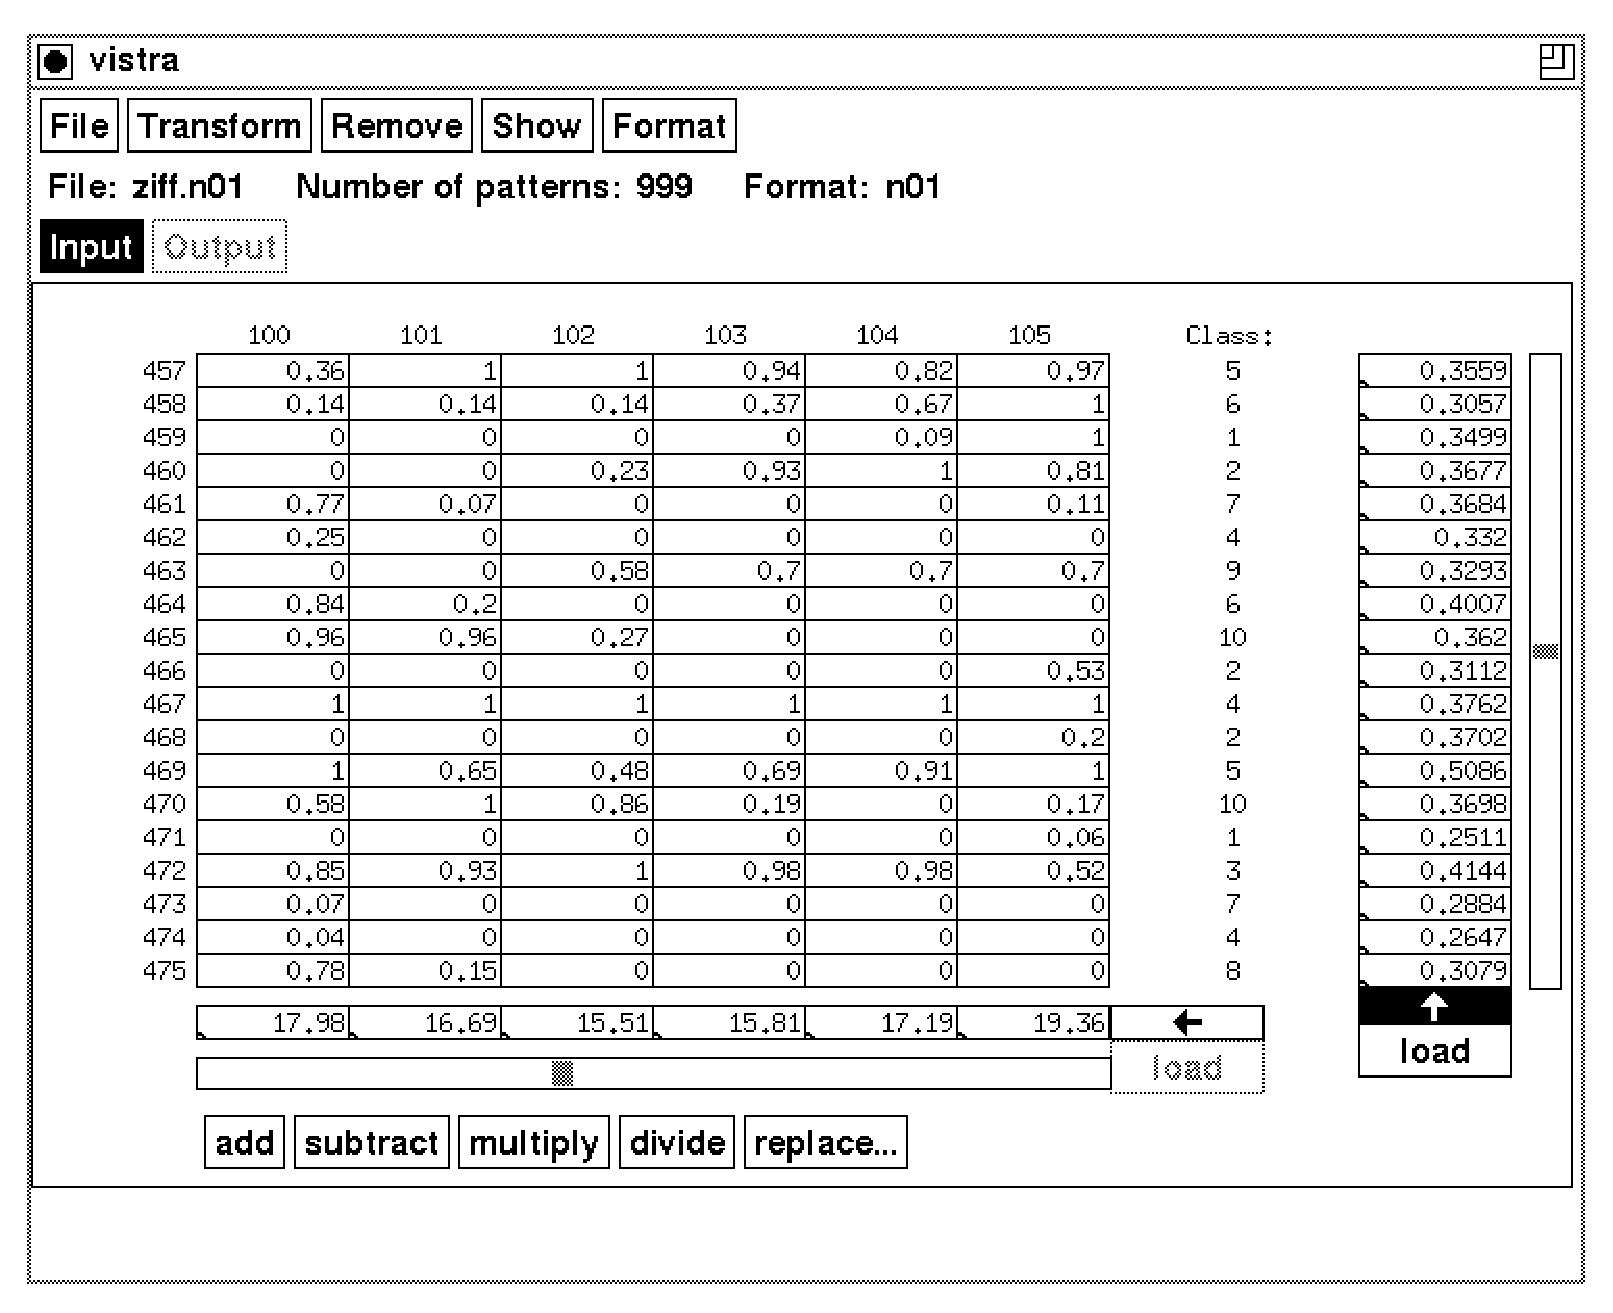
\psfig{file=main.ps,width=\textwidth,height=14cm}}
\caption{\label{hauptfenster} Das Hauptfenster von Vistra}
\end{figure}  

Das Hauptfenster ist in folgende Zonen eingeteilt:
\begin{itemize}
\item Direkt unter der Titelleiste befindet sich die {\bf Men"uleiste}, die
Men"u-Buttons f"ur das "`File"'-, "`Transform"'-, "`Remove"'-, "`Show"'- und 
"`Format"'-Men"u enth"alt.

\item Unterhalb der Men"uleiste folgt eine {\bf Info-Zeile}, die den Namen der
momentan geladenen Trainingsvektor-Datei, die Anzahl der Trainingsvektoren
sowie das momentan ausgew"ahlte Dateiformat anzeigt.

\item Es folgen {\bf zwei Buttons}, die mit "`Input"' bzw.~"`Output"' 
bezeichnet sind. 
Da im Hauptfenster immer nur ein Satz von Vektoren bearbeitet werden kann,
dienen diese Buttons zum Umschalten zwischen Eingabe- und Ausgabevektoren.
"Uber den Men"upunkt "`Input/output vectors"' des "`Show"'-Men"us
kann jedoch ein zweites Fenster ge"offnet werden, in dem immer diejenigen
Vektoren angezeigt werden, die momentan nicht im Hauptfenster bearbeitet 
werden (siehe auch Abschnitt~\ref{ssw}).
Ein Mausklick auf den "`Input"'- bzw. den "`Output"'-Button bewirkt 
ein Austauschen der beiden Fensterinhalte.

\item Ein {\bf Spreadsheet}, das entweder die Eingabe- oder die
Ausgabevektoren enth"alt.
Jede Zeile des Gitters entspricht einem Vektor.
Die Nummern der zum jeweiligen Zeitpunkt sichtbaren Vektoren sind
links neben dem Gitter angebracht.
Unmittelbar oberhalb des Gitters stehen die Nummern der sichtbaren
Dimensionen. \\
In Abbildung~\ref{hauptfenster} werden z.B. momentan die Dimensionen
100 bis 105 der Vektoren 457 bis 475 angezeigt.
Mithilfe der vertikalen bzw.~der horizontalen Scrollbars rechts 
bzw.~unterhalb des Gitters, k"onnen alle Vektorelemente bequem 
durchgebl"attert werden.

\begin{sloppypar}
Unmittelbar rechts neben dem Spreadsheet ist eine Spalte mit der
"Uberschrift "`class:"' zu sehen.
Sie enth"alt die Namen bzw.~Symbole der Klassen, denen die Vektoren
der entsprechenden Zeilen angeh"oren.
Sind keine Klassensymbole geladen, so sind an dieser Stelle die
zugeh"origen Klassennummern aufgef"uhrt. 
\end{sloppypar}

\item Direkt unterhalb bzw.~rechts neben dem Spreadsheet befinden sich 
{\bf horizontale bzw.~vertikale Skalarfelder}.
Sie dienen \ldots

\begin{enumerate}
\item zur Anzeige von Skalar-Werten, die aus den Zeilen-
bzw.~Spaltenvektoren des Spreadsheets abgeleitet werden.
Die vertikalen Felder werden dabei mit Skalaren gef"ullt, die
sich aus den Zeilenvektoren, also Eingabe- oder Ausgabevektoren,
ergeben.
Die horizontalen Felder beziehen sich hingegen auf die Spaltenvektoren
des Spreadsheets und enthalten daher Informationen "uber die einzelnen
Dimensionen der Vektoren.
\item als skalare Operanden zur Durchf"uhrung von Operationen
mit den Vektoren der Spreadsheet (Zeilen- oder Spaltenvektoren).
\end{enumerate}

Immer wenn neue Trainingsvektoren geladen werden bzw. von Eingabe- auf
Ausgabevektoren umgeschaltet wird (oder umgekehrt), werden alle 
vertikalen und horizontalen Skalarfelder auf den Wert "`0"' gesetzt.
Sp"ater k"onnen diese Felder auf zwei Arten mit Werten gef"ullt werden:

\begin{itemize}
\item von Hand mithilfe der Tastatur (dazu mu"s der Maus-Zeiger "uber
dem Eingabefeld stehen).
\item "uber einen Men"upunkt des "`Load"'-Men"us.
\end{itemize}

"Uber das "`Load"'-Men"u k"onnen Mittelwerte, Minima, Standardabweichungen
etc. von Vektoren oder Dimensionen berechnet werden.
Eine vollst"andige Liste der angebotenen Funktionen ist im
Abschnitt~\ref{loadmenu} zu finden.
Die Pfeile, die in Richtung der Skalarfelder zeigen, fungieren als
Schalter, mit denen zwischen den vertikalen und horizontalen Feldern
mittels Mausklick umgeschaltet wird.

Sind beispielsweise die vertikalen Felder selektiert, so beziehen sich
die Funktionen des "`Load"'-Men"us auf die Zeilen der Spreadsheet.
Die Minimum-Funktion des "`Load"'-Men"us w"urde die vertikalen Skalarfelder
mit dem jeweiligen minimalen Element des zugeh"origen Eingabe- bzw.
Ausgabevektors laden. 
Sind hingegen die horizontalen Felder ausgew"ahlt, so w"urden sie 
nach Ausf"uhrung der Minimum-Funktion die minimalen Elemente der einzelnen 
Dimensionen enthalten.

\item Mithilfe der {\bf Skalaroperations-Buttons} direkt unterhalb der 
horizontalen Scrollbar
werden die Zeilen- bzw.~Spaltenvektoren mit den Inhalten der vertikalen
bzw.~horizontalen Skalarfelder kombiniert.
Auch hier mu"s die Richtung der Operation vorher durch die Pfeile
eingestellt werden.
Sind die vertikalen Skalarfelder selektiert, so wird der $i$-te 
Zeilenskalar f"ur die Operation mit dem $i$-ten Zeilenvektor 
verwendet.
Sind hingegen die horizontalen Skalarfelder selektiert, so werden die
Spaltenskalare mit den Spaltenvektoren der Spreadsheet kombiniert.  
Folgende Vektor--Skalar Operationen sind m"oglich: 

\begin{tabular}{ll}
{\bf "`add"'} & elementweise Addition des Skalars \\
{\bf "`subtract"'} & elementweise Subtraktion des Skalars \\
{\bf "`multiply"'} & elementweise Multiplikation des Skalars \\
{\bf "`divide"'} & elementweise Division durch den Skalar \\
{\bf "`replace\ldots"'} & Ersetzen eines bestimmten Elements durch den Skalar \\
\end{tabular}

Im Falle von "`replace\ldots"' "offnet sich eine Dialogbox, in der
die Nummer des zu ersetzenden Elements angegeben werden mu"s.
Die "`replace\ldots"'-Funktion entspricht praktisch dem Ersetzen
einer Zeile bzw.~Spalte des Spreadsheets durch die Inhalte der horizontalen
bzw.~vertikalen Skalarfelder.

\item Der Platz unterhalb der Skalaroperations-Buttons dient zur
Anzeige von Mitteilungen "uber Operationen, Berechnungen usw., die
Vistra momentan durchf"uhrt.

"`Loading patterns\ldots"' beispielsweise besagt,
da"s Vistra zur Zeit eine Trainingsvektor-Datei einliest und deshalb
mit weiteren Benutzereingaben gewartet werden sollte.
\end{itemize}

Au"ser den Vektor--Skalar Operationen werden alle Aktionen des Hauptfensters
"uber entsprechende Men"upunkte aufgerufen.
Die folgenden Abschnitte beschreiben alle Aktionen Men"u f"ur Men"u. 
Generell gilt, da"s Operationen, deren Bezeichnungen auf "`\ldots"' enden, 
nicht sofort ausgef"uhrt werden, sondern zun"achst Dialogboxen "offnen,
in denen der Benutzer zus"atzliche Angaben zur Operation machen mu"s.  

\subsection{Das "`Load"'-Men"u}
\label{loadmenu}

Wie bereits erw"ahnt, dient das "`Load"'-Men"u zum Laden der
vertikalen oder der horizontalen Skalarfelder.
Mithilfe der beiden Pfeile k"onnen die zu ladenden Felder
ausgew"ahlt werden.
Unter jedem Pfeil befindet sich ein mit "`load"' gekennzeichneter
Men"ubutton, "uber den das "`Load"'-Men"u aufgerufen werden kann.

"Uber das "`Load"'-Men"u k"onnen sowohl skalare Werte zu den einzelnen
Vektoren bzw. Dimensionen bestimmt werden als auch globale Werte,
die von {\sl allen} Vektoren abh"angen (wie z.B. das minimale Element aller
Vektoren). 

Die ersten sieben Men"upunkte berechnen die Skalare aus den zugeh"origen
Zeilenvektoren (falls die vertikalen Felder selektiert sind), oder
aus den Spaltenvektoren des Spreadsheets
(falls die horizontalen Felder selektiert sind).  

\begin{samepage}
Sie lauten: \\
\begin{tabular}{lp{10.5cm}}
{\bf Men"upunkt} & {\bf geladen wird\ldots} \\[1ex]
"`minimum"' & das kleinste Element des Vektors \\
"`maximum"' & das gr"o"ste Element des Vektors \\
"`average"' & der Mittelwert der Vektorelemente \\
"`length"' & die L"ange des Vektors \\
"`standard deviation"' & die Standardabweichung $\sigma$ des 
Vektors $v$: \newline
\vspace{1ex}
\[ \sigma(v) = \sqrt{\frac{1}{dims} \sum_{i=1}^{dims} 
(v_{i} - \overline{v})^{2}} \]
\vspace{1ex}
\begin{tabbing}
$dims$ \qquad \= Dimensionalit"at von $v$ \\
$v_{i}$ \> $i$-tes Element von $v$ \\
$\overline{v}$ \> Mittelwert von $v$ 
\end{tabbing} \\
"`sum"' & die Summe aller Elemente des Vektors \\
"`pattern\ldots"' & das $i$-te Element des Vektors, wobei $i$ durch
den Benutzer in einer Dialogbox festgelegt wird 
\end{tabular}
\end{samepage}

Die n"achsten f"unf Men"upunkte f"ullen alle horizontalen bzw.~vertikalen
Skalarfelder mit einer Konstanten: \\

\nopagebreak
\begin{tabular}{lp{9.5cm}}
{\bf Men"upunkt} & {\bf geladen wird\ldots} \\[1ex]
"`overall minimum"' & das kleinste Element {\sl aller} Vektoren \\
"`overall maximum"' & das gr"o"ste Element {\sl aller} Vektoren \\
"`overall average"' & der Mittelwert der Elemente {\sl aller Vektoren} \\
"`overall std dev"' & die globale Standardabweichung $\sigma_{global}$
der Elemente {\sl aller} Vektoren $v_{i}$: \newline
\vspace{1ex}
\[ \sigma_{global} = \sqrt{\frac{1}{n\cdot dims} \sum_{i=1}^{n}
\sum_{j=1}^{dims} (v_{ij} - \overline{v})^{2}} \] 
\vspace{1ex}
\begin{tabbing}
$dims$ \qquad \= Dimensionalit"at der Vektoren $v_{i}$ \\
$n$ \> Anzahl der Vektoren in dem Spreadsheet \\
$v_{ij}$ \> $j$-tes Element des Vektors $v_{i}$ \\
$\overline{v}$ \> globaler Mittelwert ("`overall average"')      
\end{tabbing} \\
"`constant\ldots"' & eine beliebige Konstante, die vom Benutzer in einer 
Dialogbox eingegeben wird 
\end{tabular}

\subsection{Das "`Format"'-Men"u}

Vistra kann eine Vielzahl von Dateiformaten f"ur Trainingsvektoren lesen
und schreiben.
Neben dem LVQ- und dem N01-Format, die standardm"a"sig vorhanden sind,
handelt es sich um benutzerdefinierte ASCII-Formate, 
um die Vistra erweitert werden kann (wie in Kapitel~\ref{fdl} beschrieben).
Beim Lesen bzw.~Schreiben von Trainingsvektoren mu"s der Benutzer daher
das zu verwendende Format festlegen.
Dies geschieht "uber das "`Format"'-Men"u, in dem die Namen aller
dem Programm bekannten Formate aufgelistet sind.
 
Zu jedem Zeitpunkt ist ein Format selektiert und durch einen Haken links
vom Namen gekennzeichnet.
Zus"atzlich wird das ausgew"ahlte Format auch in der Info-Zeile angezeigt.
Die ersten drei Men"upunkte lauten "`see suffix"', "`lvq"' und "`n01"'.
"`see suffix"' bezeichnet hierbei kein bestimmtes Format, sondern legt fest, 
da"s das zu verwendende Format jeweils durch
die Endung des Dateinamens bestimmt ist.
Ist "`see suffix"' selektiert und soll z.B.~die Vektordatei "`ziffern.n01"'
geladen werden, so geht Vistra davon aus, da"s diese Datei im N01-Format
vorliegt.

Ab dem vierten Men"upunkt erscheinen die Namen der benutzerdefinierten
Formate.
Als Namen dienen hierbei die Dateinamen der FDL-Beschreibungen ohne
die Endung "`.fmt"'.  
 
\subsection{Das "`File"'-Men"u}

"Uber das "`File"'-Men"u k"onnen alle Vistra-Funktionen aufgerufen werden,
die mit dem Lesen oder dem Schreiben von Dateien zutun haben. 

\begin{description}
\item["`Load patterns\ldots"':] \mbox{} \\  
Lade neue Trainingsvektoren. \\
Es "offnet sich eine Dialogbox, in der der Name der Vektor-Datei
anzugeben ist.
Ist im "`Format"'-Men"u "`see suffix"' eingestellt, so gibt die Endung
des Dateinamens an, welches Format die Datei besitzt.

\item["`Write patterns\ldots"':] \mbox{} \\
Schreibe die bearbeiteten Trainingsvektoren in eine 
Trai\-nings\-vek\-tor-Datei. \\
Es "offnet sich eine Dialogbox, in der der Name der zu schreibenden Datei
anzugeben ist.
Ist im "`Format"'-Men"u "`see suffix"' eingestellt, so gibt die Endung
des Dateinamens an, in welchem Format die Trainingsvektoren geschrieben 
werden.

\item["`Load symbols\ldots"':] \mbox{} \\
Lade eine neue Symboltabelle. \\
Die Funktion ordnet den Klassennummern neue Symbole zu.
Die Symbole m"ussen dazu in einer Symboltabellen-Datei untergebracht sein.
Eine solche Symboltabellen-Datei hat Zeilenstruktur, wobei
die erste Zeile das erste Symbol enth"alt, die zweite Zeile das
zweite Symbol etc. 
Eine genaue Beschreibung des Formats findet sich im Abschnitt~\ref{symtab}.
Der Namen der Symboltabellen-Datei wird "uber eine Dialogbox vom Benutzer
erfragt.

Am Beispiel des xor-Problems soll dieser Proze"s veranschaulicht
werden. \\
Folgende Daten seien vor dem Laden im Speicher: 

\begin{tabular}{ccc}
{\sl Trainingsvektor} & {\sl Klassennummer} & {\sl Klassensymbol} \\[1ex]
{\tt 0 0} & {\tt 1} & {\tt NULL} \\
{\tt 0 1} & {\tt 2} & {\tt EINS} \\
{\tt 1 0} & {\tt 2} & {\tt EINS} \\
{\tt 1 1} & {\tt 1} & {\tt NULL} \\
\end{tabular}  

Die Symbole {\tt NULL} und {\tt EINS} sollen nun durch die Symbole
{\tt FALSE} und {\tt TRUE} ersetzt werden.
Dazu wird eine Symboltabellen-Datei mit folgendem Inhalt geladen: 
\begin{verbatim}
FALSE
TRUE
\end{verbatim}
Nach dem Laden liegen folgende Daten vor: 

\begin{tabular}{ccc}
{\sl Trainingsvektor} & {\sl Klassennummer} & {\sl Klassensymbol} \\[1ex]
{\tt 0 0} & {\tt 1} & {\tt FALSE} \\
{\tt 0 1} & {\tt 2} & {\tt TRUE} \\
{\tt 1 0} & {\tt 2} & {\tt TRUE} \\
{\tt 1 1} & {\tt 1} & {\tt FALSE} \\
\end{tabular}  

Mit der "`Load symbols\ldots"'-Funktion k"onnen Symbole nicht nur
ersetzt werden, sondern "uberhaupt erst einmal geladen werden.
Dies ist, wie bereits erw"ahnt, f"ur Trainingsvektoren sinnvoll, die 
im N01-Format geladen wurden, da das Format nur Klassennummern enth"alt.

Enth"alt eine Symboltabellen-Datei weniger Symbole als unterschiedliche
Klassen existieren, so erscheint eine Fehlermeldung.

\item["`Write symbols\ldots"':] \mbox{} \\
Schreibe die Symboltabelle in eine Symboltabellen-Datei. \\
Der Namen dieser Datei wird vom Benutzer "uber eine Dialogbox erfragt.
Ausgegeben werden die Klassensymbole oder, falls keine geladen sind,
die Ausgabevektoren (siehe Abschnitt~\ref{symtab}).
Existieren weder Symbole noch Ausgabevektoren, so werden einfach die
Klassennummern geschrieben.
  
\item["`Write to log file"':] \mbox{} \\ 
Dieser Men"upunkt stellt einen Schalter 
dar, wobei ein Haken anzeigt, ob die Funktion ein- oder abgeschaltet ist.
Solange sie eingeschaltet ist, werden alle Transformationen, die
auf den Eingabe- oder Ausgabevektoren durchgef"uhrt werden, in einer
LOG-Datei festgehalten.
Zu einem sp"ateren Zeitpunkt k"onnen die durchgef"uhrten Transformationen
dann mit denselben oder anderen Trainingsvektoren wiederholt werden.
Die Funktion kann w"ahrend einer Sitzung beliebig ein- oder ausgeschaltet
werden, wobei immer nur ans Ende der LOG-Datei angeh"angt wird.

Der Namen der LOG-Datei ist {\it pattern\_file\_name}{\tt\/.log},
wobei {\it pattern\_file\_name} den Namen der momentan  
geladenen Trainingsvektor-Datei repr"asentiert.
Sie wird daher in das Verzeichnis der Vektordatei gestellt.  
Das Format der LOG-Dateien wird ausf"uhrlich 
im Kapitel~\ref{log} behandelt.

\item["`Quit"':] \mbox{} \\
Beende Vistra.  
\end{description}

\subsection{Das "`Transform"'-Men"u}

Das "`Transform"'-Men"u enth"alt Funktionen zur Transformation der
Eingabevektoren oder der Ausgabevektoren, je nachdem, welche gerade
im Hauptfenster bearbeitet werden.
Es werden immer {\sl alle} Vektoren transformiert, das gezielte
Transformieren eines einzelnen Vektors ist weder zweckm"a"sig noch erlaubt. \\ 
Folgende Transformationen sind m"oglich:

\begin{description}
\item["`HLOG"':] \mbox{} \\
Es wird eine halblogarithmische 
Transformation mit den Vektoren durchgef"uhrt. \\
Sie kann nur auf Vektoren ausgef"uhrt werden, die eine quadratische
Anzahl von Dimensionen besitzen. 

Bei der Bilderkennung mit Hilfe neuronaler Netze bereiten gedrehte Objekte
besonders gro"se Probleme.
Eine Abhilfe kann die sogenannte halblogarithmische Transformation 
schaffen.
Die Vektorelemente (Bildpunkte) werden durch diese Transformation nicht
ver"andert, sondern lediglich anders angeordnet.

Man kann sich die Transformation folgenderma"sen vorstellen: \\
Man legt $b$ konzentrische Kreise mit exponentiell wachsenden Radien um den
Mittelpunkt des Bildes, wobei $b$ die Seitenl"ange des quadratischen Bildes 
in Bildpunkten ist.
Der Radius $r_i$ des $i$-ten Kreises ($i=0,1,\ldots,b-1$) betr"agt:

\[ r_i = \left( \frac{b}{2}\right)^{\frac{i}{b-1}} \qquad \mbox{Bildpunkte} \] 

Legt man nun Geraden durch den Mittelpunkt, die jeweils einen Winkel
von $\frac{2\pi}{b}$ ein\-schlie"sen, so wird die erste Spalte des neuen
Bildes aus den Bildpunkten des Originals gebildet, die im 
Gegenuhrzeigersinn unter den Schnittpunkten dieser Geraden mit dem innersten
Kreis liegen.
Die zweite Spalte erh"alt man aus den Schnittpunkten mit dem zweitinnersten 
Kreis usw.
Die Schnittpunkte mit dem "au"sersten Kreis liefern schlie"slich die Elemente 
der letzten Spalte des transformierten Bildes. 

Durch die halblogarithmische Transformation wird erreicht, da"s
Drehungen von Objekten im Original   
zu Verschiebungen im transformierten Bild f"uhren.
Verschiebungen k"onnen von neuronalen Netzen jedoch wesentlich leichter
erkannt werden.

\item["`FFT"':] \mbox{} \\
Es wird eine diskrete eindimensionale 
Fourier Transformation (FFT) auf den Vektoren durchgef"uhrt.
Diese Transformation ist nur f"ur Vektoren zul"assig, die $2^{n}$ 
($n \geq 1$) Dimensionen besitzen.

Bei der FFT handelt es sich um eine komplexwertige Vektorfunktion.
Bevor eine FFT auf einem Vektor $v$ durchgef"uhrt wird, m"ussen die
Vektorelemente $v_{i}$ deshalb zun"achst in komplexe Zahlen 
$(v_{i,real},v_{i,imag})$ "uberf"uhrt werden. \\
Dies geschieht in Vistra wie folgt:

\begin{tabular}{@{\hspace*{1cm}}lcl}
$v_{i,real}$ & := & $v_{i}$ \\
$v_{i,imag}$ & := & $0.0$ \\
\end{tabular}

Nach Durchf"uhrung der Fourier Transformation auf dem Vektor $v$
werden die komplexen Vektorelemente wieder in reelle Zahlen umgewandelt:

\hspace*{1cm} $v_{i} := \sqrt{v_{i,real}^{2} + v_{i,imag}^{2}}$

Die diskrete eindimensionale Fourier Transformation ist ausf"uhrlich
in \cite{jaehne} beschrieben. 

\item["`PCA"':] \mbox{} \\ 
Auf den Vektoren wird eine 
Haupt\-achsen-Trans\-form\-ation 
({\bf P}rinciple {\bf C}om\-po\-nent {\bf A}na\-ly\-sis) 
durchgef"uhrt. \\
F"ur eine Beschreibung sei auf \cite{hertz} oder \cite{bronstein} verwiesen. 

Vistra verwendet zur Durchf"uhrung der PCA-Transformation das 
Programm "`pca"', das Trainingsvektoren im LVQ-Format liest, die PCA
durchf"uhrt und die transformierten Vektoren anschlie"send im LVQ-Format 
nach stdout schreibt. 

Vistra schreibt daher in einem ersten Schritt die Trainingsvektoren 
im LVQ-Format in eine tempor"are Datei, ruft anschlie"send das Programm 
"`pca"' mit dieser Datei als Parameter auf, lenkt die Ausgabe auf 
eine weitere tempor"are Datei um und liest diese 
schlie"slich wieder im LVQ-Format ein.

\item["`Normalize"':] \mbox{} \\
Alle Vektoren des Spreadsheets werden 
normalisiert, d.h.~jeder Vektor $v$ 
wird elementweise durch seine L"ange $|v|$ dividiert, so da"s jeder Vektor
anschlie"send die L"ange $|v|=1$ besitzt:
 
\[ v := \frac{v}{|v|} \]

Diese Transformation kann auch leicht mithilfe der Skalarfelder 
durchgef"uhrt werden.
Zuerst l"adt man die vertikalen Skalarfelder mit den L"angen der Vektoren
(Men"upunkt "`length"' des "`Load"'-Men"us).
Anschlie"send wird der "`divide"'-Button gedr"uckt.

\item["`Scale\ldots"':] \mbox{} \\
Die Elemente aller Vektoren werden 
auf einen neuen Wertebereich skaliert, der in einer Dialogbox anzugeben ist. 

Die Skalierung erfolgt derart, da"s das kleinste Element des Spreadsheets
("`overall minimum"') auf die untere Intervallgrenze und das gr"o"ste
("`overall maximum"') auf die obere Intervallgrenze abgebildet wird.

\item["`Randomize"':] \mbox{} \\
Die Reihenfolge der Trainingsvektoren wird willk"urlich ver"andert.

\item["`Expand with class vector"':] \mbox{} \\
Jeder Vektor des Spreadsheets wird mit seinem Klassenvektor erweitert. 

Unter Klassenvektor versteht man dabei einen Vektor bestehend aus Nullen
und Einsen, wobei die Anzahl der Dimensionen der Anzahl unterschiedlicher
Klassen entspricht. 
Das $i$-te Element des Klassenvektors ist genau dann 1, wenn der
Trainingsvektor die Klassennummer $i$ besitzt, sonst 0. 

Das Erweitern durch die Klassenvektoren soll am xor-Beispiel veranschaulicht
werden. \\
Links sind die Vektoren vor und rechts nach der Transformation zu
sehen: 

\nopagebreak
\begin{tabular}{ccc}
{\sl Eingabevektoren vorher} & {\sl Klassen-Nr.} & 
{\sl Eingabevektoren nachher} \\[1ex] 
{\tt 0 0} & {\tt 1} & {\tt 0 0 1 0} \\  
{\tt 0 1} & {\tt 2} & {\tt 0 1 0 1} \\  
{\tt 1 0} & {\tt 2} & {\tt 1 0 0 1} \\  
{\tt 1 1} & {\tt 1} & {\tt 1 1 1 0} \\  
\end{tabular}
 
\item["`Expand with output vector"':] \mbox{} \\
Diese Transformation kann nur durchgef"uhrt werden, wenn 
Ausgabevektoren existieren.
Die Vektoren des Spreadsheets werden mit den Elementen des 
zugeh"origen Ausgabevektors erweitert.

\item["`Refresh class numbers"':] \mbox{} \\
Es werden die Klassennummern anhand der Ausgabevektoren neu berechnet. \\ 
Diese Funktion kann nur aufgerufen werden, wenn keine Klassensymbole geladen
sind.

Trainingsvektoren mit gleichen Ausgabevektoren erhalten die gleichen
Klassennummern.
Die vergebenen Nummern sind 1, 2,\ldots, $n$ , wobei $n$ 
der Anzahl unterschiedlicher Ausgabevektoren entspricht.
\end{description}
 
\subsection{Das "`Remove"'-Men"u}

Das "`Remove"'-Men"u h"alt Funktionen bereit, mit denen Trainingsvektoren
oder bestimmte Dimensionen der Vektoren entfernt werden k"onnen:

\begin{description}
\item["`Dimensions\ldots"':] \mbox{} \\
Es wird ein Bereich von Dimensionen (also Spalten des Spreadsheets) entfernt. \\
Dazu "offnet sich eine Dialogbox, in der die erste und die letzte der
zu entfernenden Dimensionen anzugeben ist.
Es k"onnen nicht alle Dimensionen entfernt werden.

\item["`Constant dims"':] \mbox{} \\
Es werden alle konstanten Dimensionen, also alle Spalten des
Spread\-sheets, 
in denen alle Elemente die gleichen Werte besitzen, entfernt.
Sind alle Dimensionen konstant, so kann die Operation nicht
ausgef"uhrt werden.

\item["`Vectors\ldots"':] \mbox{} \\
Es wird eine Reihe von Trainingsvektoren entfernt. \\
In einer Dialogbox ist der Nummernbereich der zu entfernenden Vektoren
zu spezifizieren.
Es k"onnen jedoch nicht alle Trainingsvektoren gel"oscht werden.
\end{description}

\subsection{Das "`Show"'-Men"u} 

Neben dem Hauptfenster existieren weitere Fenster, die alle "uber
einen entsprechenden Men"upunkt des "`Show"'-Men"us ge"offnet werden. \\
Folgende Men"upunkte stehen zur Verf"ugung:

\nopagebreak
\begin{description}
\item["`Graphics"':] \mbox{} \\
Es wird ein Graphik-Fenster ge"offnet. 
Ein Graphik-Fenster kann wahlweise die Ein\-ga\-be- oder die Ausgabevektoren
in einer von f"unf verschiedenen Darstellungsarten graphisch darstellen.
Es k"onnen beliebig viele solcher Graphik-Fenster ge"offnet werden.
Dadurch ist es m"oglich, ein und denselben Vektor 
auf mehrere Arten gleichzeitig wiederzugeben.
   
\item["`Statistics"':] \mbox{} \\
Es wird ein Fenster ge"offnet, das statistische Informationen "uber die
geladenen Trai\-nings\-vek\-to\-ren anzeigt.

\item["`Covariance matrix"':] \mbox{} \\
Es wird ein Fenster ge"offnet, 
das die Kovarianzmatrix der im Hauptfenster befindlichen Vektoren
anzeigt.

\item["`Input/output vectors"':] \mbox{} \\
Es wird ein Fenster ge"offnet, in dem die Eingabevektoren oder die
Ausgabevektoren textuell dargestellt werden. 
Dieses Fenster enth"alt immer genau diejenigen Vektoren, die momentan
nicht im Hauptfenster bearbeitet werden.
Auf diese Weise k"onnen zugeh"orige Eingabe- und Ausgabevektoren
gleichzeitig betrachtet werden.
\end{description}

Die folgenden Abschnitte zeigen diese Fenster nun der Reihe nach und
geben Hinweise zu deren Benutzung.
  
\subsection{Die Graphik-Fenster}

Zu jedem Zeitpunkt k"onnen mehrere Graphik-Fenster ge"offnet sein.
Jedes dieser Fenster kann Vektoren in einer der folgenden f"unf
Darstellungsarten graphisch wiedergeben:

\begin{itemize}
\item als Histogramm
\item als Linienzug
\item als Grauwertbild
\item als Farbbild
\item als 2-dimensionale Projektion
\end{itemize} 

Zwischen diesen Darstellungsarten kann beliebig umgeschaltet werden.
Auch die Gr"o"se der Abbildungen kann man innerhalb gewisser Grenzen
ver"andern.
Abbildung~\ref{grayMat} zeigt ein Graphik-Fenster, das momentan 
auf "`gray matrix"' eingestellt ist und einen Vektor als Grauwertbild
darstellt.

\begin{figure}[ht]
\centerline{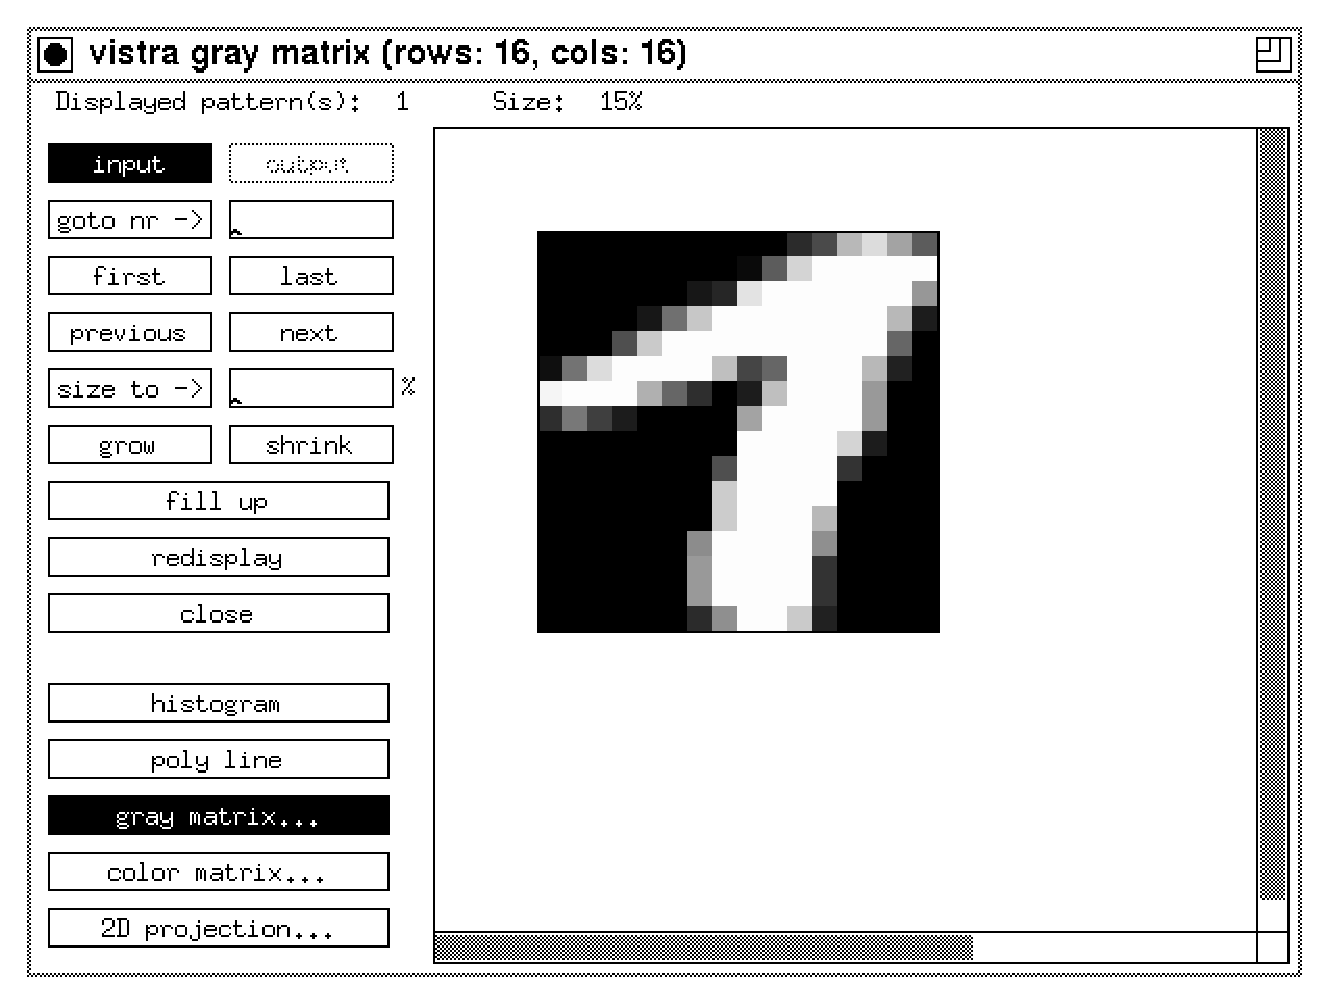
\psfig{file=gray.ps,width=\textwidth,height=10cm}}
\caption{\label{grayMat} Graphik-Fenster mit Grauwertbild}
\end{figure}

Der Titel des Fensters gibt an, welche Darstellungsart momentan gew"ahlt ist.
Unterhalb der Titelleiste erscheint eine Zeile, die Auskunft "uber die
Nummer des abgebildeten Vektors und die Gr"o"se der Abbildung (in \%
der Maximalgr"o"se) gibt.
F"ur die 2-dimensionale Projektion wird anstelle einer Vektor-Nummer
der String "`all"' angezeigt, da diese Darstellungsart alle Vektoren
gemeinsam in einer einzigen Graphik bzw.~Koordinatensystem wiedergibt. 

Am linken Rand des Graphik-Fensters befinden sich eine Reihe von 
Kommando-Buttons.
Durch sie werden Aktionen zum "`Durchbl"attern"' der Vektoren, zur
Ver\-gr"o"ser\-ung/Ver\-kleiner\-ung der Darstellungen oder zum Umschalten
zwischen Eingabe- und Ausgabevektoren bzw.~zum Umschalten zwischen den
verschiedenen Darstellungsarten, ausgef"uhrt. \\
Tabelle~\ref{gwcomms} beschreibt die Buttons des Graphik-Fensters.

\begin{table}[ht]
\begin{tabular}{lp{10.8cm}}
{\bf Button} & {\bf Aktion} \\ \hline
"`input"' & zeige einen Eingabevektor \\
"`output"' & zeige einen Ausgabevektor \\
"`goto nr --$>$"' & zeige den Vektor mit der Nummer, die das Eingabefeld rechts
daneben enth"alt \\
"`first"' & zeige den Vektor Nummer~1 \\
"`last"' & zeige den Vektor mit der h"ochsten Nummer \\
"`previous"' & zeige den vorhergehenden Vektor \\
"`next"' & zeige den n"achsten Vektor \\
"`size to --$>$"' & zeichne die Graphik in $i$ Prozent der Maximalgr"o"se, wobei
$i$ ins Eingabefeld rechts daneben einzutragen ist \\
"`grow"' & vergr"o"sere die Graphik \\
"`shrink"' & verkleinere die Graphik \\
"`fill up"' & nutze den Platz rechts und unterhalb des Diagramms zur 
gleichzeitigen Darstellung weiterer Vektoren.
"Uber jedem Diagramm befindet sich die Nummer des dargestellten Vektors.
Abbildung~\ref{fillup} zeigt ein Graphik-Fenster, das die Vektoren 1 bis 999
als Grauwertbilder minimaler Gr"o"se wiedergibt (1 Pixel pro Vektorelement).
  \\
"`redisplay"' & aktualisiere die Graphik (die dargestellten Vektoren
wurden im Hauptfenster seit dem letzten Zeichnen evtl.~modifiziert;
die graphische Darstellung w"are in diesem Fall veraltet) \\
"`close"' & schlie"se das Graphik-Fenster \\
"`histogram"' & zeige den Vektor als Histogramm \\
"`poly line"' & zeige den Vektor als Linienzug \\
"`gray matrix\ldots"' & zeige den Vektor als Grauwertbild. 
Die Anzahl der Zeilen und Spalten wird "uber eine Dialogbox durch den 
Benutzer festgelegt. \\
"`color matrix\ldots"' & zeige den Vektor als Farbbild.
Die Anzahl der Zeilen und Spalten wird "uber eine Dialogbox durch den
Benutzer festgelegt. \\
"`2D projection\ldots"' & stelle alle Vektoren in einem gemeinsamen
2-dimensionalen Koordinatensystem dar.
Der Benutzer legt in einer Dialogbox fest, welche Dimension die x-Werte
und welche Dimension die y-Werte liefern soll. 
\end{tabular}
\caption{\label{gwcomms} Die Buttons des Graphik-Fensters}
\end{table}

\begin{figure}[ht]
\centerline{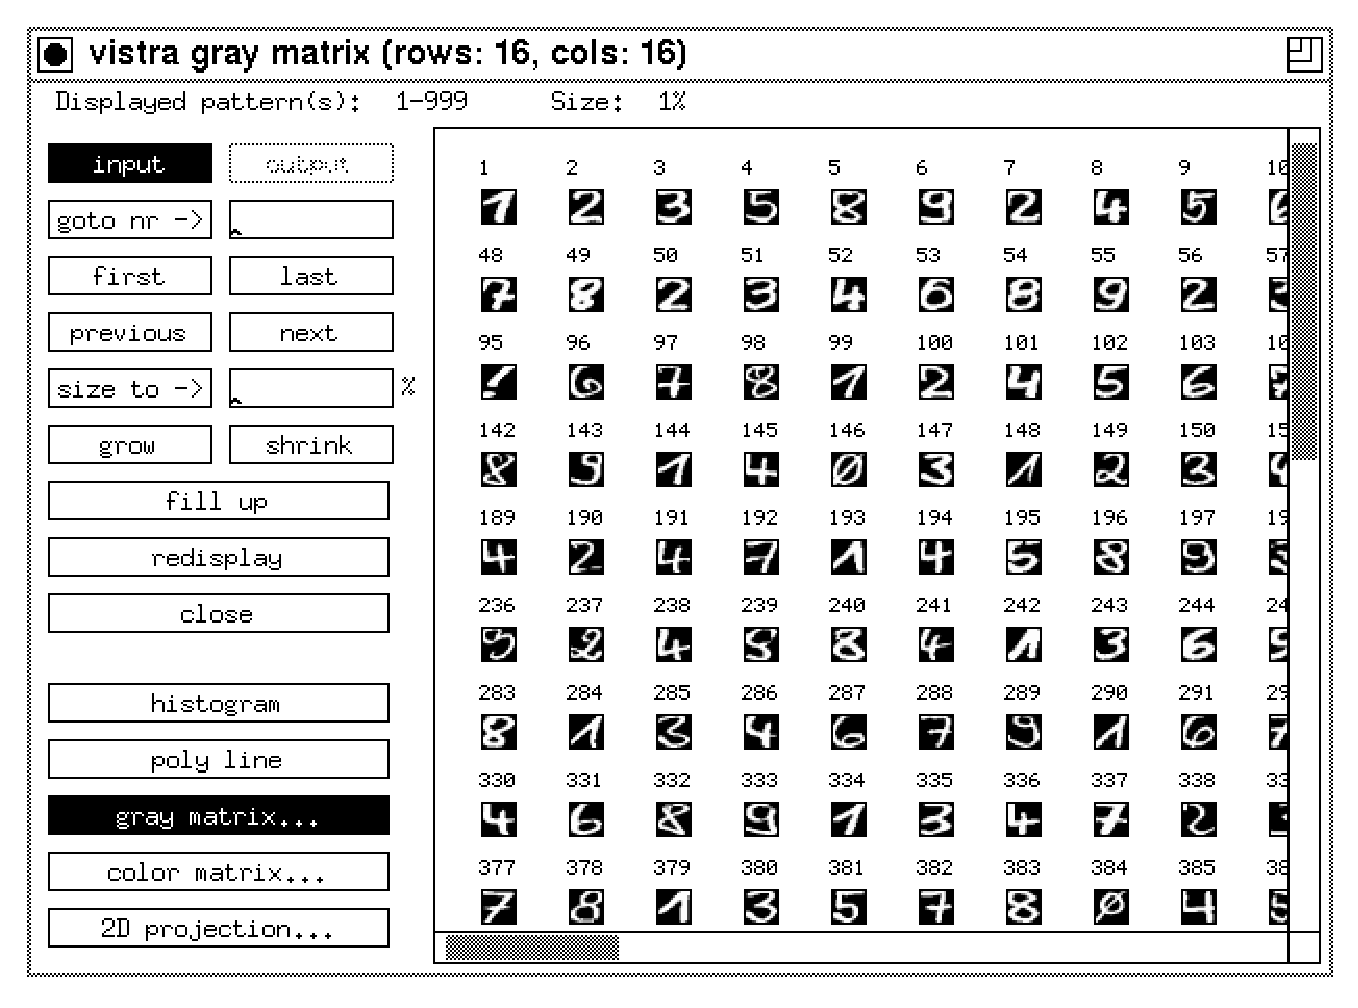
\psfig{file=fillup.ps,width=\textwidth,height=10cm}}
\caption{\label{fillup} Gleichzeitige Darstellung mehrerer Vektoren}
\end{figure}

{\bf WICHTIG:} Auch w"ahrend ein oder mehrere Graphik-Fenster ge"offnet 
sind, k"onnen die Vektoren im Hauptfenster weiterhin bearbeitet
bzw.~transformiert werden.
Aus diesem Grund ist es m"oglich, da"s ein Graphik-Fenster eine 
"`alte Version"' eines Vektors wiedergibt. 
Um sicherzustellen, da"s die Darstellung auf dem neuesten Stand ist,
sollte ein "`redisplay"' durchgef"uhrt werden oder irgendein anderer
Button gedr"uckt werden, der ein Neuzeichnen der Graphik bewirkt
(z.B.~"`next"', "`grow"' etc.). 

\subsection{Die Darstellungsarten}

\subsubsection*{Histogramm}

Ein Histogramm stellt eine Art "`Treppenfunktion"' in einem 
zweidimensionalen Koordinatensystem dar. 
Dabei liefert jedes Element $v_{i}$ des Vektors den Funktionswert 
f"ur den Bereich $[i\!-\!1,i]$ der x-Achse.
Abbildung~\ref{histo} zeigt ein Graphik-Fenster, das ein
Histogramm wiedergibt.
Der dargestellte Vektor besitzt 32 Dimensionen und ist das Ergebnis
einer vorausgegangen Fourier-Transformation.

\begin{figure}[ht]
\centerline{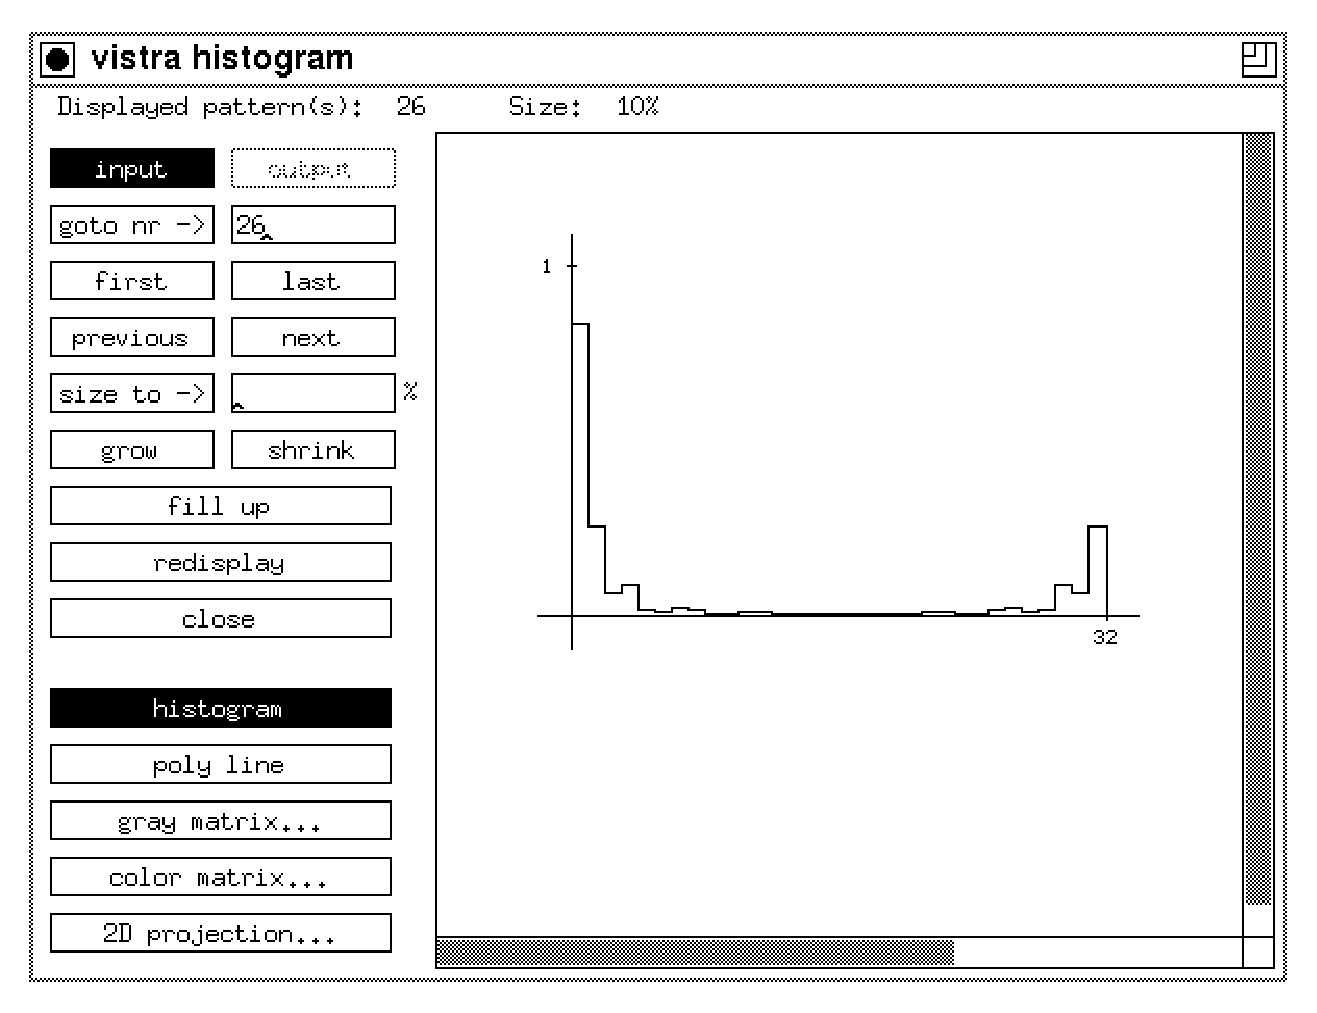
\psfig{file=histo.ps,width=\textwidth,height=10cm}}
\caption{\label{histo} Histogramm-Darstellung eines Vektors}
\end{figure} 

W"ahrend die H"ohe des Histogramms konstant bleibt, kann die Breite
"uber die entsprechenden Buttons des Graphik-Fensters ("`size to --$>$"',
"`grow"' oder "`shrink"') ver"andert werden.
Um die minimale Breite zu erhalten, gibt man als Gr"o"se "`0\%"' an.
Eine L"angeneinheit der x-Achse ist dann 1~Pixel breit.
 
\subsubsection*{Linienzug}

Ein Linienzug ist einem Histogramm sehr "ahnlich. 
Auch er wird in ein zweidimensionales Koordinatensystem gezeichnet.
Die Vektorelemente $v_{i}$ liefern dabei die Punkte $(i,v_{i})$, die
durch Linien verbunden werden.
Abbildung~\ref{poly} zeigt eine Linienzug-Darstellung des Vektors aus
Abbildung~\ref{histo}.

\begin{figure}[ht]
\centerline{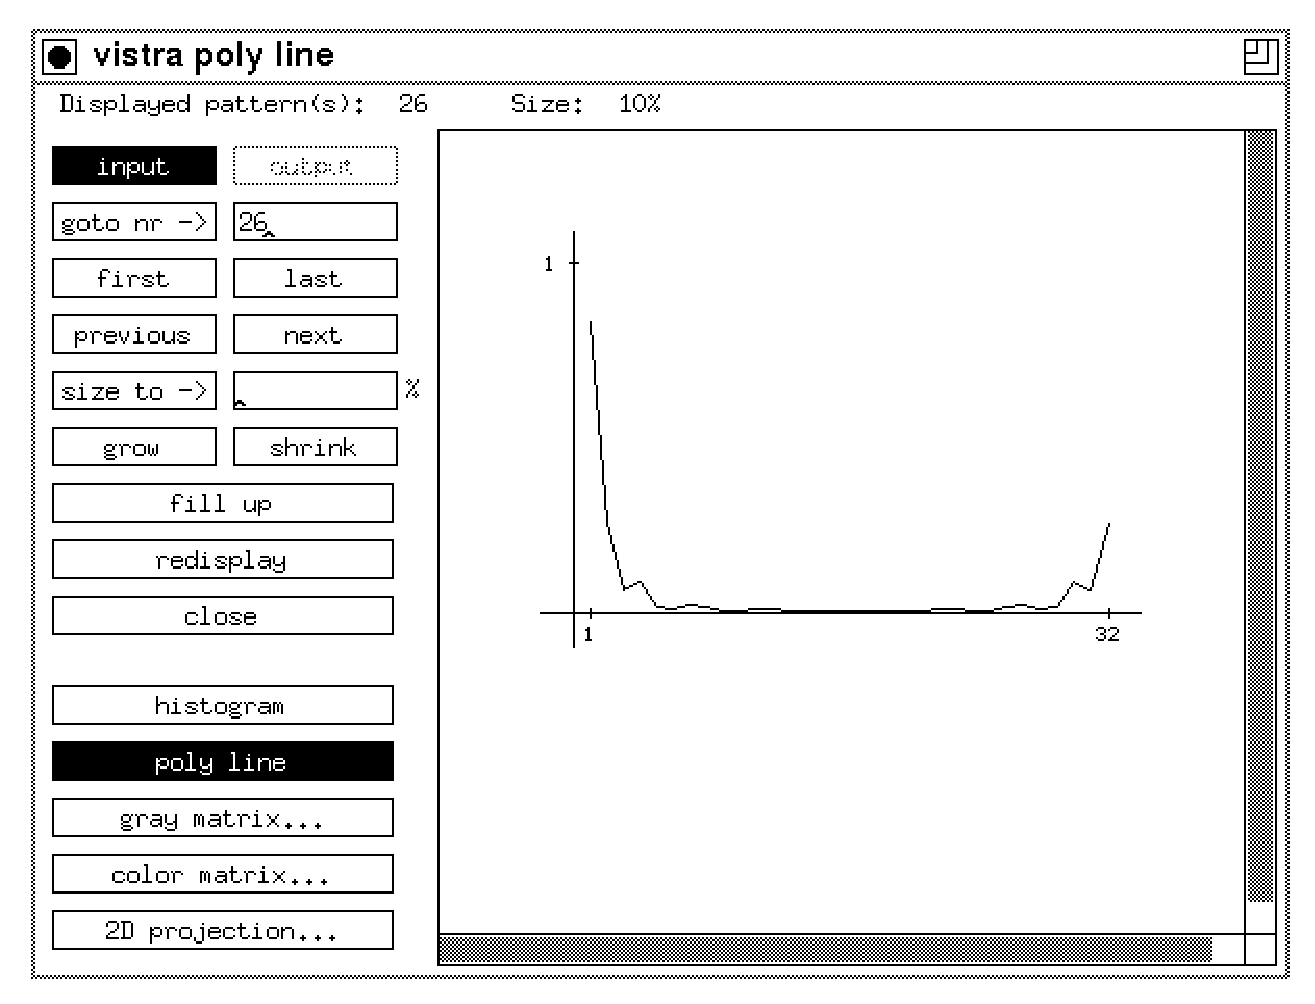
\psfig{file=poly.ps,width=\textwidth,height=10cm}}
\caption{\label{poly} Linienzug-Darstellung eines Vektors}
\end{figure} 

Die x-Achse kann "uber die entsprechenden Buttons des Graphik-Fensters
gedehnt oder geschrumpft werden.
Eine L"angeneinheit der x-Achse ist im Minimalfall genau ein Pixel breit. 

\subsubsection*{Grauwertbild}

Abbildung~\ref{grayMat} zeigte bereits ein Grauwertbild eines Vektors.
Der dargestellte Vektor besitzt 256 Dimensionen, die in eine Matrix
mit 16~Zeilen und 16~Spalten eingeteilt wurden.
Jedes Vektorelement wird durch ein Quadrat repr"asentiert, das in einem
bestimmten Grauton gezeichnet ist.
Das kleinste Element aller Eingabevektoren (bzw.~Ausgabevektoren)
erh"alt dabei die geringste Intensit"at und wird daher schwarz dargestellt.
Das gr"o"ste Element erh"alt die h"ochste Intensit"at und erscheint wei"s.
Werte dazwischen werden je nach Gr"o"se in einem Grauton dargestellt. 

Die Anzahl der Zeilen~bzw.~Spalten der Matrix wird vom Benutzer festgelegt. 
Die Anzahl der Zellen mu"s jedoch mindestens so gro"s wie die Dimensionalit"at
des abzubildenden Vektors sein.
Die ersten Elemente des Vektors werden durch die erste Zeile der Matrix
repr"asentiert, die n"achsten durch die zweite Zeile etc.
"`"Ubersch"ussige"' Zellen werden wei"s dargestellt. 

Die Elemente $v_{1}, \ldots, v_{7}$ eines 7-dimensionalen Vektors w"urden
wie folgt auf eine 3x3-Matrix verteilt werden:

\hspace*{2cm}
\begin{tabular}{|c|c|c|}
\hline $v_{1}$ & $v_{2}$ & $v_{3}$ \\
\hline $v_{4}$ & $v_{5}$ & $v_{6}$ \\
\hline $v_{7}$ & & \\ \hline
\end{tabular}    
 
Die Gr"o"se der quadratischen Zellen kann "uber die entsprechenden Buttons
des Graphik-Fensters ver"andert werden.
Die Minimalgr"o"se betr"agt ein Pixel. 

\subsubsection*{Farbbild}

Die Darstellung eines Vektors als Farbbild erfolgt analog der
Grauwert-Darstellung.
Einziger Unterschied ist die Verwendung des gesamten Farbspektrums
anstelle von Graut"onen.

\subsubsection*{2D-Projektion}

Die 2D-Projektion ist die einzige Darstellungsart, in der
{\it alle} Vektoren in einer einzigen Graphik wiedergegeben sind.
Jeder Vektor wird als ein Punkt in ein zweidimensionales Koordinatensystem
eingetragen.
Der Benutzer legt fest, welche Dimension der Vektoren die x-Werte und
welche die y-Werte liefert.

Abbildung~\ref{proj2D} zeigt ein Beispiel, in dem die Dimensionen~2 und 1
von insgesamt 10~000 Vektoren abgebildet sind.
Die Gr"o"se des Schaubilds kann "uber die entsprechenden Buttons des 
Graphik-Fensters variiert werden.

\begin{figure}[ht]
\centerline{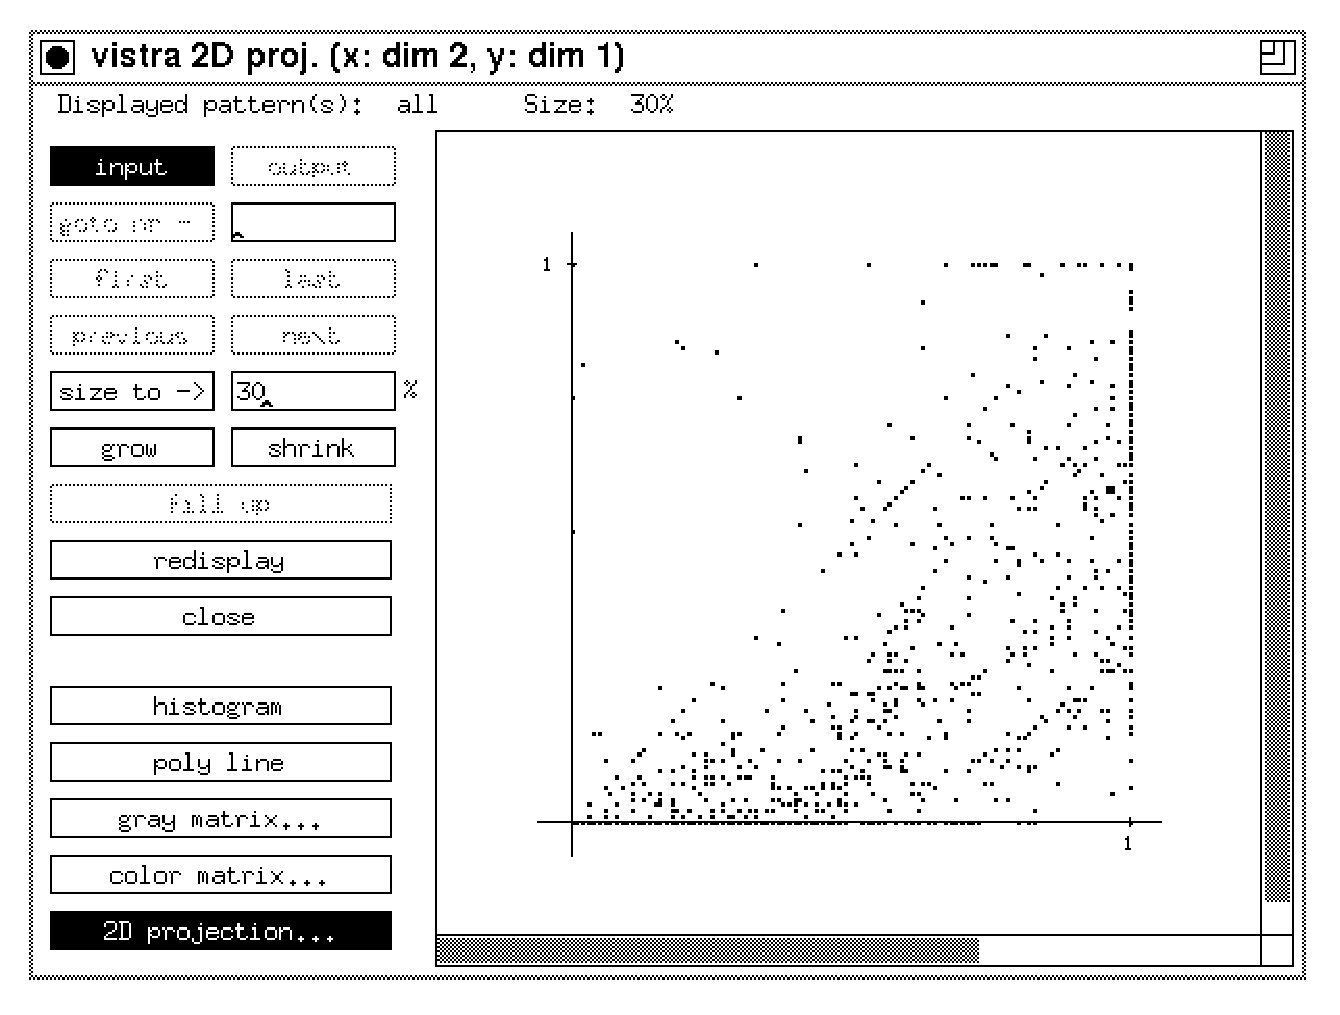
\psfig{file=proj2D.ps,width=\textwidth,height=10cm}}
\caption{\label{proj2D} Projektion zweier Dimensionen}
\end{figure}
 
\subsection{Das Statistik-Fenster}

Das Statistik-Fenster liefert allgemeine und statistische Informationen
"uber die geladenen Trainingsvektoren.
Abbildung~\ref{statistics} zeigt ein Beispiel.

\begin{figure}[ht]
\centerline{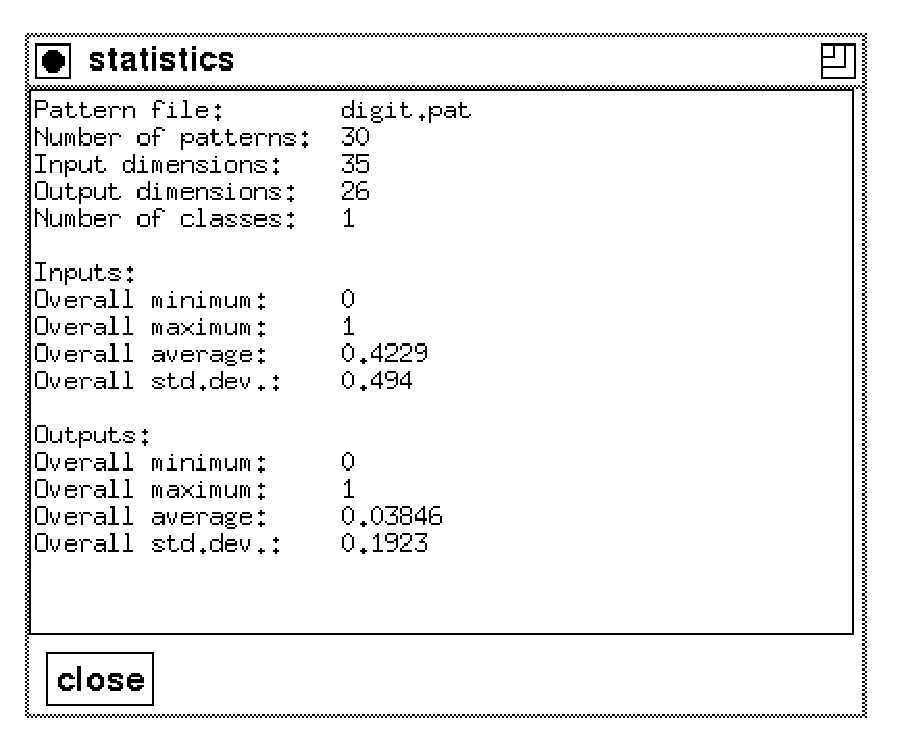
\psfig{file=stat.ps,width=10cm,height=8cm}}
\caption{\label{statistics} Das Statistik-Fenster}
\end{figure}

Der erste Teil zeigt allgemeine Informationen zu die Trainingsvektoren.
Die weiteren Abschnitte enthalten statistische Daten "uber 
die Eingabe- und Ausgabevektoren, wie sie auch "uber die "`Load"'-Men"us
des Hauptfensters berechnet werden k"onnen.  

Das Statistik-Fenster mu"s "uber "`close"' geschlossen werden, bevor
im Hauptfenster weitergearbeitet werden kann.

\subsection{Das Kovarianzmatrix-Fenster}

Das Kovarianzmatrix-Fenster zeigt eine Matrix, die alle Kovarianzen
zwischen je zwei Dimensionen der im Hauptfenster befindlichen Vektoren
enth"alt.
Stellt $nvecs$ die Anzahl der Vektoren und $ndims$ die Anzahl der
Dimensionen dar, so wird eine 
$ndims\times\/ndims$-Matrix $cov$ berechnet, in der das
Element $cov_{ij}$ die Kovarianz der Dimensionen $i$ und $j$ enth"alt. \\
Sei $avg_{i}$ der Mittelwert der Dimension $i$
($avg_{i} = \frac{1}{nvecs} \sum_{k=1}^{nvecs} v_{ki}$,  
$v_{k}$: $k$-ter Vektor), so berechnet sich $cov_{ij}$ wie folgt:

\[ cov_{ij} = \frac{1}{nvecs} \sum_{k=1}^{nvecs} 
(v_{ki} - avg_i)(v_{kj} - avg_j) 
\]    

F"ur $i=j$ erh"alt man aus obiger Formel:
\begin{displaymath}
cov_{ii} = \frac{1}{nvecs} \sum_{k=1}^{nvecs} 
(v_{ki} - avg_i)^{2}
\end{displaymath}
$cov_{ii}$ stellt also gerade die Varianz $\sigma^{2}_{i}$
der Dimension $i$ dar.
Die Matrix $cov$ ist au"serdem spiegelsymmetrisch, da f"ur alle $i,j$
gilt: $cov_{ij} = cov_{ji}$.

Abbildung~\ref{covariances} zeigt das Kovarianzmatrix-Fenster, das
die Kovarianzen f"ur folgende Vektoren enth"alt:

\nopagebreak
\begin{tabular}{l@{\hspace{1cm}}l}
{\sl Vektor~1:} & {\tt 0 2 1} \\
{\sl Vektor~2:} & {\tt 3 2 2} \\
{\sl Vektor~3:} & {\tt 1 2 3} \\
{\sl Vektor~4:} & {\tt 0 2 2} \\
\end{tabular}

\begin{figure}[ht]
\centerline{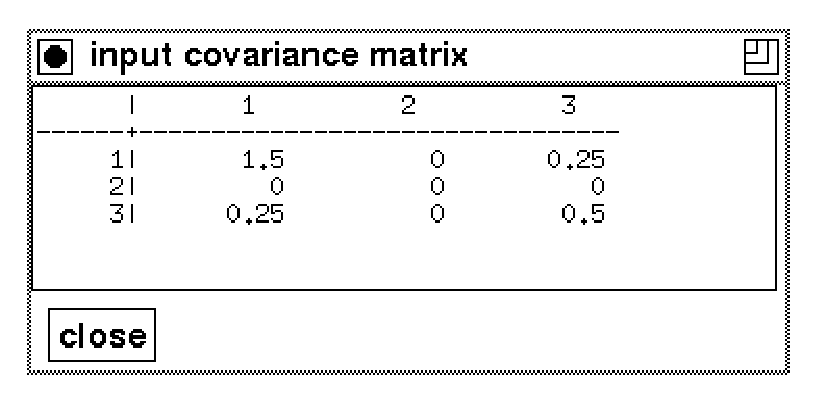
\psfig{file=cov.ps,width=8cm,height=4cm}}
\caption{\label{covariances} Das Kovarianzmatrix-Fenster}
\end{figure}

\subsection{Das Vektoren-Fenster}
\label{ssw}

Das Vektoren-Fenster kann nur ge"offnet werden, wenn Eingabe- und 
Ausgabevektoren vorhanden sind. 
Werden im Hauptfenster die Eingabevektoren (Ausgabevektoren) bearbeitet, 
so enth"alt das Vektoren-Fenster die Ausgabevektoren (Eingabevektoren).
Die Vektoren k"onnen im Vektoren-Fenster nur gelesen werden, 
Transformationen sind nur im Hauptfenster m"oglich.
Abbildung~\ref{vektorfenster} zeigt ein Vektoren-Fenster, in dem
momentan die Dimensionen 17 bis 22 der Vektoren 1 bis 22 angezeigt werden.
Der Titel des Fensters besagt, da"s es sich hierbei um die
Eingabevektoren handelt. 
"Uber den "`close"'-Button wird das Fenster wieder geschlossen. 

\begin{figure}[ht]
\centerline{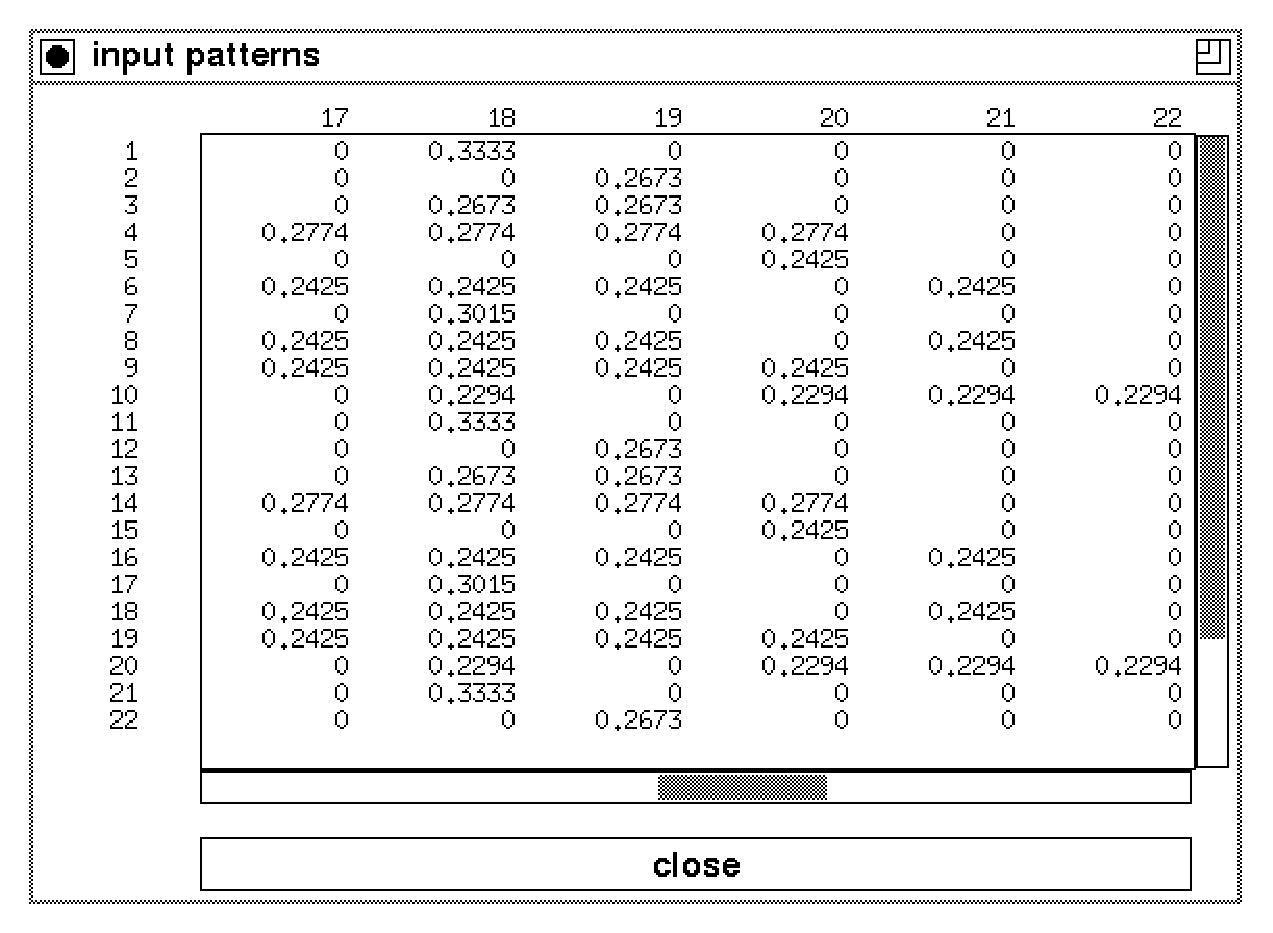
\psfig{file=readsh.ps,width=\textwidth,height=8cm}}
\caption{\label{vektorfenster} Das Vektoren-Fenster}
\end{figure}




 \clearpage
\clearpage \section{Batch-Modus und LOG-Dateien}
\label{log}

Der Aufruf von Vistra im Batch-Modus wurde bereits in Abschnitt~\ref{call}
behandelt.
Dieses Kapitel beschreibt, wie LOG-Dateien zur Spezifikation eines 
durchzuf"uhrenden Jobs zu verwenden sind.

Eine LOG-Datei stellt eine Liste von Kommandos zur Transformation
von Trainingsvektoren dar.
Alle Transformationen, die interaktiv durchgef"uhrt werden, k"onnen 
mithilfe von LOG-Dateien auch im Stapelbetrieb durchgef"uhrt werden.
F"ur jede Transformation steht daf"ur ein entsprechendes Batch-Kommando
zur Verf"ugung.
Der Batch-Modus von Vistra erh"alt als Eingabe eine Trainingsvektor-Datei
und eine LOG-Datei, arbeitet die Befehle der LOG-Datei der Reihe nach
ab und schreibt die transformierten Trainingsvektoren wieder in eine
Ausgabe-Datei.  

Dem Batch-Modus fallen zwei Aufgaben zu:
\begin{itemize}
\item Transformationen k"onnen sowohl interaktiv "uber die X-Windows 
Oberfl"ache als auch als Job im Stapelbetrieb durchgef"uhrt werden.
Dazu ist eine LOG-Datei von Hand zu erstellen.
\item Der Batch-Modus erm"oglicht eine Trennung in
Trainings- und Testdaten oder ganz allgemein eine Aufteilung von
Trainingsvektoren in separate Dateien.
Die Transformationen, die interaktiv auf einen Satz der Trainingsvektoren 
angewandt werden, k"onnen in einer LOG-Datei festgehalten
werden, indem das Flag "`Write to log file"' des "`File"'-Men"us
gesetzt wird.
Sp"ater k"onnen die anderen Dateien durch Angabe dieser LOG-Datei 
im Batch-Modus auf die gleiche Weise umgewandelt werden.
\end{itemize}  
   
\subsection{Das Format von LOG-Dateien}

LOG-Dateien besitzen eine Zeilenstruktur.
Jede Zeile enth"alt eine Anweisung bzw. eine durchzuf"uhrende 
Transformation und besteht
aus ein oder mehreren W"ortern bzw. Zahlen, die
durch Blanks oder Tabulatoren getrennt sind.
Die Syntax einer Befehlszeile ist:

{\tt ('i'|'I'|'o'|'O') <command> [ <arg1> <arg2> ... ]}  

oder

{\tt \% <comment>}

Das erste Wort einer Zeile mu"s also immer ein einzelnes Zeichen sein.
Ein {\tt i} bzw. {\tt I} bedeutet, da"s die Anweisung auf die Eingabevektoren
anzuwenden ist, ein {\tt o} bzw. {\tt O}, da"s sie sich auf die
Ausgabevektoren bezieht. 
Generell wird in LOG-Dateien nicht zwischen Gro"s- und
Kleinschreibung unterschieden. \\  
{\tt \%} leitet eine Kommentarzeile ein. 
Alle Zeichen dieser Zeile werden von Vistra ignoriert.   

{\tt <command>} steht f"ur ein Schl"usselwort, das angibt, welche
Aktion bzw. Transformation durchzuf"uhren ist.

Manche Anweisungen ben"otigen zur genaueren Spezifikation einen oder
mehrere Parameter, die in obiger Syntax durch die Liste 
{\tt <arg1> <arg2> ...} repr"asentiert werden. 
Parameter k"onnen sowohl Strings als auch Zahlen sein.
 
F"ur jede Aktion, die im interaktiven Modus
Trainingsvektoren ver"andert, steht ein entsprechendes Batch-Kommando
zur Verf"ugung.
Neben Kommandos f"ur die Transformationen des "`Transform"'-Men"us und
des "`Remove"'-Men"us"' existieren auch f"ur das Laden der vertikalen
und horizontalen Skalarfelder (also f"ur jeden Men"upunkt des "`Load"'-Men"us)
sowie f"ur die Vektor--Skalar Operationen ("`add"', "`subtract"', "`multiply"',
"`divide"' und "`replace\ldots"') entsprechende Batch-Anweisungen.
W"ahrend eine LOG-Datei abgearbeitet wird, merkt sich Vistra neben den
aktuellen Werten der Trainingsvektoren auch die Inhalte der vertikalen
und horizontalen Skalarfelder zu den verschiedenen Zeitpunkten.

{\bf Beispiel:} \\
Mithilfe einer LOG-Datei sollen die Elemente der Trainingsvektoren auf
den Wertebereich [-1,1] skaliert werden.
Anschlie"send ist von jedem Vektorelement der statistische Mittelwert
der zugeh"origen Dimension abzuziehen. 
Zum Schlu"s soll noch eine Hauptachsentransformation (PCA) durchgef"uhrt
werden. 

\begin{samepage}
Diese Transformationen k"onnten im Batch-Modus durch folgende LOG-Datei
vollzogen werden:
\begin{verbatim}
i scale -1 1
% Mittelwerte der Dimensionen sollen 0 sein
i loadHoriz avg
i subtract horiz
% zum Schluss: Hauptachsentransformation
i pca
\end{verbatim}  
\end{samepage}
 
Tabelle~\ref{batchcommands} zeigt alle Batch-Anweisungen plus zugeh"orige
Parameter.

\begin{table}
\begin{tabular}{c|c|p{7.5cm}}
{\tt <command>} & {\tt <arg1> <arg2> ...} & {\bf Aktion} \\ \hline
{\tt pca} & & Hauptachsentransformation \\
{\tt fft} & & 1-dimensionale diskrete Fourier Trans\-for\-ma\-tion \\
{\tt hlog} & & halblogarithmische Transformation \\
{\tt scale} & {\it min\quad max} & skaliere aufs Intervall 
[{\it min}, {\it max}] \\
{\tt normalize} & & normalisiere auf L"ange 1 \\
{\tt randomize} & & mische die Vektoren willk"urlich \\
{\tt classExpand} & & erweitere mit Klassenvektor \\
{\tt outputExpand} & & erweitere mit Ausgabevektor \\
{\tt refreshClasses} & & berechne die Klassen aus den
Aus\-ga\-be\-vek\-toren \\
{\tt rmDimRange} & {\it from\quad to} & entferne die Dimensionen {\it from} 
bis {\it to} \\
{\tt rmConstDims} & & entferne alle konstanten Dimensionen \\
{\tt rmDims} & $dim_1 \ldots dim_n$ & entferne die Dimensionen 
$dim_1, \ldots, dim_n$ \\ 
{\tt loadVert} & {\it loadparams} & lade die vertikalen Skalarfelder 
je nach {\it loadparams} mit bestimmten Werten (siehe unten) \\
{\tt loadHoriz} & {\it loadparams} & lade die horizontalen Skalarfelder 
je nach {\it loadparams} mit bestimmen Werten (siehe unten) \\
{\tt add} & {\it direction} & addiere die vertikalen 
({\it direction} = {\tt vert})
bzw. die horizontalen ({\it direction} = {\tt horiz}) Skalare zu den 
zugeh"origen Vektoren bzw. Dimensionen \\
{\tt subtract} & {\it direction} & subtrahiere die vertikalen 
({\it direction} = {\tt vert}) bzw. die horizontalen 
({\it direction} = {\tt horiz}) 
Skalare von den zugeh"origen Vektoren bzw. Dimensionen \\
{\tt multiply} & {\it direction} & multipliziere die vertikalen 
({\it direction} = {\tt vert}) bzw. die horizontalen 
({\it direction} = {\tt horiz}) 
Skalare mit den zugeh"origen Vektoren bzw. Dimensionen \\
{\tt divide} & {\it direction} & dividiere die Vektoren 
({\it direction} = {\tt vert})
bzw. die Dimensionen ({\it direction} = {\tt horiz}) durch die zugeh"origen 
vertikalen bzw. horizontalen Skalare \\
{\tt replace} & {\it direction\quad nr} & ersetze den Vektor Nummer~{\it nr} 
({\it direction} = {\tt horiz}) bzw. die Dimension~{\it nr} 
({\it direction} = {\tt vert}) durch die horizontalen 
bzw. vertikalen Skalare \\
{\tt addConst} & {\it num} & addiere {\it num} zu jedem Vektorelement \\
{\tt subConst} & {\it num} & subtrahiere {\it num} von jedem Vektorelement \\
{\tt multConst} & {\it num} & multipliziere jedes Vektorelement mit 
{\it num} \\
{\tt divConst} & {\it num} & dividiere jedes Vektorelement durch {\it num} \\ 
\end{tabular}
\caption{\label{batchcommands} Die Batch-Anweisungen}
\end{table}
  
Durch die Batch-Anweisungen {\tt loadVert} und {\tt loadHoriz} k"onnen
die vertikalen bzw. horizontalen Skalarfelder mit Werten geladen werden.
Unter anderem stehen alle Funktionen zur Verf"ugung, die auch interaktiv "uber
das "`Load"'-Men"u aufgerufen werden k"onnen. 

{\it loadparams} aus Tabelle~\ref{batchcommands} kann folgende Werte
annehmen: 

\nopagebreak
\begin{tabular}{c|c}
{\it loadparams} & {\bf entspricht "`Load"'-Men"upunkt\ldots} \\ \hline
{\tt min} & "`minimum"' \\
{\tt max} & "`maximum"' \\
{\tt avg} & "`average"' \\
{\tt length} & "`length"' \\
{\tt sum} & "`sum"' \\
{\tt stddev} & "`standard deviation"' \\
{\tt pattern} {\it nr} & "`pattern\ldots"' \\
{\tt overallMin} & "`overall minimum"' \\
{\tt overallMax} & "`overall maximum"' \\
{\tt overallAvg} & "`overall average"' \\
{\tt overallStddev} & "`overall std dev"' \\
{\tt const} {\it number} & "`const\ldots"' \\
{\tt values} $val_1 \ldots val_n$ & --- \\
{\tt dim} \enspace $nr$ \enspace $value$ & --- \\  
\end{tabular} 

F"ur die Anweisung {\tt const} gibt {\it number} die zu ladende Konstante an.
Die Anweisung {\tt pattern} l"adt den Vektor Nummer {\it nr}
in die horizontalen Skalarfelder ({\tt <command> = loadHoriz})
bzw. die {\it nr}-te Dimension in die vertikalen Felder 
({\tt <command> = loadVert}). \\
Durch {\tt values} k"onnen die Werte, mit denen die vertikalen bzw.
horizontalen Skalarfelder geladen werden sollen, direkt angegeben werden.
Diese Werte wurden in obiger Tabelle mit $val_1 \ldots val_n$ bezeichnet.
$n$ mu"s dabei genau der Anzahl der betreffenden Skalarfelder
entsprechen. \\
Wie f"ur {\tt values} gibt es auch f"ur die Anweisung {\tt dim} keine
Entsprechung im "`Load"'-Men"u.
Mit {\tt dim} wird das $nr$-te vertikale ({\tt <command> = loadVert})
bzw. das $nr$-te horizontale Skalarfeld ({\tt <command> = loadHoriz})
auf den Wert $value$ gesetzt.
{\tt dim} entspricht im interaktiven Modus somit einer "Anderung 
eines Skalarfeldes von Hand.
F"ur jedes ge"anderte Feld wird eine {\tt dim}-Anweisung in die LOG-Datei
geschrieben.   
 
\subsubsection*{Fehlerbehandlung im Batch-Modus}

Trifft Vistra in der LOG-Datei auf eine Zeile mit fehlerhafter Syntax,
so wird eine Warnung auf stdout ausgegeben und mit der 
n"achsten Zeile fortgefahren.
Gleiches gilt f"ur Anweisungen, die aus anderen Gr"unden 
nicht ausgef"uhrt werden k"onnen.
Eine halblogarithmische Transformation ben"otigt beispielsweise Vektoren
mit einer quadratischen Anzahl von Dimensionen.
Ein weiteres Beispiel ist die {\tt loadVert values}-Anweisung, die
eine Warnung erzeugt, wenn die Anzahl der Werte nicht der Anzahl
der Trainingsvektoren entspricht. 

\subsection{LOG-Anweisungen der interaktiven Aktionen}

Dieser Abschnitt besch"aftigt sich mit der Frage, welche LOG-Anweisungen
f"ur die Aktionen, die interaktiv im Hauptfenster von Vistra 
durchgef"uhrt werden, in die LOG-Datei geschrieben werden, solange 
"`Write to log file"' gesetzt ist.
Dabei ist zu beachten, da"s eine Trennung von Trainingsvektoren nur
dann sinnvoll unterst"utzt wird, wenn ein und derselbe Vektor durch
Ausf"uhrung der LOG-Datei in genau der gleichen Weise ver"andert wird wie 
durch die interaktiv durchgef"uhrten Transformationen.

Vektor-Transformationen, deren Ergebnisse nur vom jeweiligen Vektor 
abh"angen, bereiten unter diesem Gesichtspunkt keine Probleme
(z.B. liefert eine Fourier Transformation auf den gleichen Vektor angewandt
immer das gleiche Resultat).
Schwierigkeiten machen jedoch Aktionen, die von {\it allen} geladenen
Vektoren abh"angen.
Darunter f"allt beispielsweise das Entfernen konstanter Dimensionen.
Eine Dimension, die f"ur eine Menge von Vektoren konstant ist, mu"s
nicht auch f"ur andere Vektormengen konstant sein.
W"urde in diesem Fall einfach nur {\tt rmConstDims} in die LOG-Datei
geschrieben, so k"onnten den Vektoren einer Datei evtl. ganz andere Dimensionen
entfernt werden als den Trainingsvektoren einer anderen Datei. 
Abhilfe kann nur geschaffen werden, wenn die LOG-Datei  
die tats"achlich entfernten Dimensionen explizit enth"alt (mithilfe
von {\tt rmDims}).      

"Ahnlich verh"alt es sich, wenn z.B. die horizontalen Skalarfelder 
mit den Minima der einzelnen Dimensionen geladen werden sollen.
Die Minima k"onnen je nach Vektormenge anders ausfallen, weshalb auch
hier anstelle von {\tt loadHoriz min} 
das Minimum jeder Dimension explizit in die LOG-Datei geschrieben wird.

Folgende Tabelle enth"alt in der linken Spalte die 
interaktiven Aktionen und in der rechten die daf"ur geschriebenen 
LOG-Anweisungen:

\begin{tabular}{l|l}
{\bf Men"upunkt/Button} & {\bf geschriebene LOG-Anweisung(en)} \\ \hline
"`HLOG"' & {\tt hlog} \\
"`FFT"' & {\tt fft} \\
"`PCA"' & {\tt pca} \\
"`Normalize"' & {\tt normalize} \\
"`Scale"' & {\tt multConst} {\it stretch} \\
& {\tt addConst} {\it shift} \\
"`Randomize"' & {\tt randomize} \\
"`Expand with class vector"' & {\tt classExpand} \\
"`Expand with output vector"' & {\tt outputExpand} \\
"`Refresh class numbers"' & {\tt refreshClasses} \\
"`Remove dimensions"' & {\tt rmDimRange} {\it from to} \\
"`Remove constant dims"' & {\tt rmDims} $dim_1 \ldots dim_n$ \\
"`add"' & {\tt add} {\it direction} \\
"`subtract"' & {\tt subtract} {\it direction} \\
"`multiply"' & {\tt multiply} {\it direction} \\
"`divide"' & {\tt divide} {\it direction} \\
"`replace"' & {\tt replace} {\it nr} \\
\end{tabular}

Eine Skalierung eines Wertebereichs auf einen anderen kann auf
eine Multiplikation und eine Addition zur"uckgef"uhrt werden.
Der betreffende Faktor bzw. Summand ist oben als {\it stretch} bzw.
{\it shift} bezeichnet. \\
{\it direction} steht entweder f"ur {\tt vert} oder f"ur {\tt horiz}.

In obiger Tabelle fehlen die Aktionen des "`Load"'-Men"us.
Bei ihnen h"angen die geschriebenen LOG-Anweisungen davon ab, ob die vertikalen
oder die horizontalen Skalarfelder geladen wurden:

\begin{tabular}{l|l|l}
{\bf "`Load"'-Men"upunkt} & {\bf vertikal} & {\bf horizontal} \\ \hline
"`minimum"' & {\tt loadVert min} & {\tt loadHoriz values} {\it valueList} \\
"`maximum"' & {\tt loadVert max} & {\tt loadHoriz values} {\it valueList} \\
"`average"' & {\tt loadVert avg} & {\tt loadHoriz values} {\it valueList} \\
"`length"' & {\tt loadVert length} & {\tt loadHoriz values} {\it valueList} \\
"`standard deviation"' & {\tt loadVert stddev} & {\tt loadHoriz values} 
{\it valueList} \\
"`sum"' & {\tt loadVert sum} & {\tt loadHoriz values} {\it valueList} \\
"`pattern"' & {\tt loadVert values} {\it valueList} &
{\tt loadHoriz values} {\it valueList} \\
"`overall minimum"' & {\tt loadVert const} {\it value} &
{\tt loadHoriz const} {\it value} \\   
"`overall maximum"' & {\tt loadVert const} {\it value} &
{\tt loadHoriz const} {\it value} \\   
"`overall average"' & {\tt loadVert const} {\it value} &
{\tt loadHoriz const} {\it value} \\   
"`overall std dev"' & {\tt loadVert const} {\it value} &
{\tt loadHoriz const} {\it value} \\   
"`const"' & {\tt loadVert const} {\it value} & 
{\tt loadHoriz const} {\it value} \\ 
\end{tabular}

{\it valueList} repr"asentiert hierbei eine Liste von Zahlen, die jeweils 
durch ein Blank voneinander getrennt sind.
Eine letzte M"oglichkeit zur Manipulation der Skalarfelder ist 
das direkte "Andern eines Feldinhalts von Hand mithilfe der Tastatur.
In diesem Fall wird einer der folgenden beiden Anweisungen in die
LOG-Datei geschrieben (je nachdem, ob es sich um ein vertikales oder
ein horizontales Skalarfeld handelt):

{\tt loadVert dim} \enspace $nr$ \enspace $value$ \qquad oder \\
{\tt loadHoriz dim} \enspace $nr$ \enspace $value$  

Das $nr$-te vertikale bzw. horizontale Skalarfeld wird hierdurch auf
den Wert $value$ gesetzt. \clearpage
\clearpage \section{Datei-Formate}
\label{formate}

Dieses Kapitel beschreibt, welche Formate die LVQ-, N01- und 
Symboltabellen-Dateien haben bzw. haben
m"ussen, wenn sie von Vistra geschrieben bzw. gelesen werden
(siehe auch \cite{bayer}).
Das Format der LOG-Dateien wurde bereits in Kapitel~\ref{log} erl"autert.
Formatbeschreibungs-Dateien sind Thema des Kapitels~\ref{fdl}, 
in der die Syntax von FDL (Format Description Language) beschrieben
wird und einige Beispiele f"ur benutzerdefinierte ASCII-Dateiformate
gegeben werden.

\subsection{Das LVQ-Format}
\label{lvq}

Das LVQ-Format ist ein sehr einfaches Trainingsvektor-Format, das eine Menge von
Eingabevektoren enth"alt und jedem dieser Vektoren ein Klassensymbol
zuordnet.

Das LVQ-Format setzt sich aus einem Kopf und einem Rumpf zusammen.
Der Kopf besteht lediglich aus einer Zeile, die die Dimensionalit"at der
Eingabevektoren enth"alt.
Der Rumpf besitzt pro Eingabevektor eine Zeile, in der die Elemente
des jeweiligen Vektors gefolgt von seinem Klassensymbol aufgef"uhrt sind.

Folgendes Beispiel zeigt ein LVQ-File, das zweidimensionale
Trainingsvektoren enth"alt, die das xor-Problem definieren:

\nopagebreak
\begin{verbatim}
2
0 0 NULL
0 1 EINS
1.0 0.0 EINS
1 1.0 NULL
\end{verbatim}
   
\subsection{Das N01-Format}
\label{n01}
Das N01-Format ist ein bin"ares Format, das geschaffen wurde, um das
Einlesen bzw. Schreiben von Trainingsvektor-Dateien zu beschleunigen.
Bei sehr gro"sen Vektor-Dateien ist es daher empfehlenswert, 
anstelle eines ASCII-Formats dieses Format zu verwenden.

Die ersten 32 Bytes stellen den Kopf des N01-Formats dar.
Er hat folgende Gestalt:

\nopagebreak
\begin{tabular}[t]{l|l|l}
{\bf Bytes} & {\bf C-Typ} & {\bf Inhalt} \\ \hline
0~--~3 & char[4] & String ''N01'' mit abschlie"sender '$\backslash0$' \\
4~--~7 & unsigned int & Dimensionalit"at der Eingabevektoren \\
8~--~11 & unsigned int & Dimensionalit"at der Ausgabevektoren \\
12~--~15 & unsigned int & Anzahl der Trainingsvektoren \\
16~--~19 & unsigned int & Offset der Eingabedaten \\
20~--~23 & unsigned int & Offset der Ausgabedaten \\
24~--~27 & unsigned int & Offset der Klassennummern \\
28~--~31 & unsigned int & Anzahl unterschiedl.~Klassen 
\end{tabular}  

Die Offsets geben die File-Positionen innerhalb der N01-Datei an, an denen
die Eingabevektoren, Ausgabevektoren oder Klassennummern beginnen.
Die Eingabe- bzw. Ausgabevektoren sind als Felder von aufeinanderfolgenden
Flie"skommazahlen von jeweils 4 Bytes (C-Typ: {\tt float}) gespeichert.
In diesen Feldern erscheinen zun"achst alle Elemente des ersten 
Eingabe- bzw. Ausgabevektors, gefolgt von den Elementen des zweiten etc.
Die Klassennummern sind in einem Feld aufeinanderfolgender
Integer von jeweils 4 Bytes L"ange untergebracht (C-Typ: {\tt unsigned int}).
Die L"ange des Felds entspricht der Anzahl der Trainingsvektoren.

Das N01-Format wurde urspr"unglich f"ur DEC Workstations eingef"uhrt,
weshalb deren Maschinencodierung von {\tt float} bzw. {\tt unsigned} Typen
verwendet wird.
Hierbei erscheint das niederwertigste Byte als erstes,
das h"oherwertigste als letztes Byte innerhalb der Datei.

Vistra kann N01-Formate jedoch in jedem Fall lesen und schreiben
(unabh"angig davon, ob es auf einer SUN oder einer DEC l"auft).
Das Programm stellt fest, ob die Maschinencodierung des Rechners, auf dem
es l"auft, mit der DEC-Codierung "ubereinstimmt.
Ist dies nicht der Fall (wie bei den Maschinen der Marke SUN), so
werden alle Daten nach dem Einlesen bzw. vor dem Schreiben der N01-Datei
in geeigneter Weise konvertiert. 
    
\subsection{Das Format der Symboltabellen}
\label{symtab}

Symboltabellen-Dateien haben eine Zeilenstruktur.
Jede Zeile enth"alt genau ein Symbol, wobei 
die $i$-te Zeile der Datei das Klassensymbol zur Klassennummer $i$ enth"alt.

Abh"angig davon, ob die geladenen Trainingsvektoren explizite
Klassensymbole besitzen (die durch Strings repr"asentiert werden) oder nicht,
ist der Inhalt der einzelnen Zeilen verschieden.

Existieren explizite Klassensymbole, so werden diese als 
Zeileninhalte verwendet.
Wurde z.B.~ein LVQ-File wie das aus Kapitel~\ref{lvq} geladen, so existieren
solche Klassensymbole. \\ 
\begin{samepage} Die Symboltabellen-Datei s"ahe wie folgt aus:
\begin{verbatim}
NULL
EINS
\end{verbatim}
\end{samepage}

Existieren keine expliziten Klassensymbole, so werden die Ausgabevektoren
als solche betrachtet.
Identische Vektoren stellen dasselbe Klassensymbol dar.
Eine Zeile der Sym\-bol\-tabel\-len-Datei besteht dann gerade aus den Elementen
eines Ausgabevektors und die
Anzahl der Zeilen der Symboltabelle entspricht genau der Anzahl der
unterschiedlichen Ausgabevektoren.
Die Ausgabevektoren werden in der Reihenfolge ausgegeben, in der sie 
zum ersten Mal in den Trainingsvektoren auftauchen.

\begin{samepage}
Eine Symboltabelle f"ur Trainingsvektoren mit zweidimensionalen 
Ausgabevektoren, die keine expliziten Klassensymbole besitzen, k"onnte
wie folgt aussehen:
\begin{verbatim}
0.1 0.9
0.9 0.9
0.9 0.1
0.1 0.1
\end{verbatim}
\end{samepage}
 \clearpage
\clearpage \section{Hinzuf"ugen neuer ASCII-Formate f"ur Vektordateien}
\label{fdl}

Vistra kann um benutzerdefinierte ASCII-Formate f"ur 
Trainingsvektor-Dateien erweitert werden.
Dazu sind folgende drei Schritte notwendig:

\begin{enumerate}
\item Erzeugen einer ASCII-Datei, die das neue Format in der 
Formatbeschreibungssprache FDL definiert.
Der Name dieser Datei mu"s auf {\tt .fmt} enden.
\item Kopieren der FDL-Datei in das Verzeichnis, das durch die 
Environment-Variable VISTRAFORMATS gegeben ist.
\item Neustarten von Vistra, um das neue Format einzubinden.
\end{enumerate}

\subsection{Die Formatbeschreibungssprache FDL}

Die Beschreibung eines Formats in FDL "ahnelt von der Struktur her 
einer Auspr"agung dieses Formats.

Der erste Unterschied besteht jedoch darin, da"s in der FDL-Beschreibung Angaben
"uber Dimensionen, die Anzahl der Vektoren etc. durch bestimmte
Steuersymbole, den sogenannten {\it Deskriptoren}, ersetzt werden.
Auch f"ur Klassensymbole, Eingabe- und Ausgabevektoren existieren
entsprechende Deskriptoren. \\ 
Der zweite Unterschied ist, da"s Wiederholungen (z.B.~eine Aufz"ahlung
aller Eingabevektoren) durch Schleifenkonstrukte dargestellt werden.

Zur Veranschaulichung soll eine FDL-Beschreibung des LVQ-Formats dienen.
Vistra be\-n"o\-tigt zwar keine FDL-Beschreibung dieses Standard-Formats, da
Lese- und Schreibroutinen festcodiert vorliegen.
Als einf"uhrendes Beispiel f"ur FDL ist sie jedoch sehr geeignet.   

\subsubsection*{Beispiel~1: FDL-Spezifikation des LVQ-Formats}
\begin{samepage} Eine FDL-Beschreibung des LVQ-Formats lautet:
\begin{verbatim}
%e <
{ %i %c < }
\end{verbatim}  
\end{samepage}
Die erste Zeile enth"alt zwei Deskriptoren.
{\tt \%e} gibt an, da"s an dieser Stelle die Dimensionalit"at der 
Eingabevektoren erscheint.
Der zweite Deskriptor {\tt <} bedeutet "`new-line"', d.h. "uberall wo
dieser Deskriptor auftaucht mu"s in der Vektor-Datei eine neue Zeile
beginnen.

Die zweite Zeile der obigen FDL-Beschreibung enth"alt eine 
{\it repetition}-Schleife.
Anfang bzw. Ende der Schleife sind durch {\tt \{} bzw. {\tt \}} markiert.
Der Rumpf besteht aus einer Liste von einem oder mehreren Deskriptoren,
in diesem Fall aus den Deskriptoren {\tt \%i}, {\tt \%c} und {\tt <}.  
Das {\it repetition}-Konstrukt repr"asentiert eine null- oder mehrmalige
Wiederholung der Deskriptoren innerhalb des Rumpfs.
Im Beispiel bedeutet dies, da"s in der Vektor-Datei zun"achst der
erste Eingabevektor gefolgt vom zugeh"origen Klassensymbol erscheint,
anschlie"send der zweite Eingabevektor mit zugeh"origem Klassensymbol
usw. 
Nach jedem Klassensymbol mu"s eine neue Zeile begonnen werden.

Neben Deskriptoren und {\it repetition}-Schleifen gibt es als letztes
FDL-Sprachmittel noch die sogenannten {\it matchOne}-Schleifen.
Eine {\it matchOne}-Schleife steht f"ur das null- oder mehrmalige
Ausw"ahlen einer Alternative.
Sie wird durch die Zeichen {\tt [} und {\tt ]} begrenzt und enth"alt im 
Rumpf eine oder mehrere Listen von Deskriptoren, die die
verschiedenen Alternativen darstellen und durch {\tt |} getrennt sind.
Die {\it matchOne}-Schleife wird verst"andlicher, wenn man sich ein
Beispiel ansieht.

\subsubsection*{Beispiel~2:}
Folgendes Format f"ur eine Vektor-Datei w"are denkbar:
\begin{itemize}
\item jede Zeile enth"alt einen Eingabevektor, einen Ausgabevektor oder
einfach einen Kommentar
\item eine Zeile, die einen Eingabevektor enth"alt, beginnt mit {\tt input:}
und wird gefolgt von den Vektorelementen
\item bei Ausgabevektoren beginnt die Zeile mit {\tt output:}
\item es spielt keine Rolle, ob zuerst die Eingabevektoren oder die
Ausgabevektoren erscheinen. 
Ein- und Ausgabevektoren d"urfen auch beliebig abwechseln.
\end{itemize}  
\begin{samepage}
Das Format w"urde in FDL wie folgt aussehen:
\begin{verbatim}
[ input:  %i < | 
  output: %o < | 
  * 
]
\end{verbatim}
\end{samepage}
Der {\tt *} ist ein Deskriptor, der f"ur einen beliebigen String bis
einschlie"slich dem
n"achsten {\it new-line}-Zeichen steht und im Beispiel~2 somit die
Kommentar-Zeilen repr"asentiert. \\
{\tt \%o} repr"asentiert einen Ausgabevektor. 

Folgende Vektor-Dateien des xor-Problems w"aren zul"assige
Auspr"agungen des Bei\-spiel-Formats~2:

\nopagebreak
\parbox[t]{6cm}{
{\sl Auspr"agung~1} \\[1ex]
{\tt Ausgabe-Muster \\
output: 0 \\
output: 1 \\
output: 1 \\
output: 0.0 \\ 
\\
Eingabe-Muster \\
input: 0.0 0.0 \\
input: 0 1 \\
input: 1.0 0 \\
und noch eins... \\
input: 1 1 }} 
\parbox[t]{6cm}{{\sl Auspr"agung~2} \\[1ex] 
{\tt die ersten 2 abwechselnd \\
input:   0  0 \\
output:  0 \\
input:   0  1 \\
output:  1 \\
die letzten 2 getrennt \\
input:   1  0 \\
input:   1  1 \\
output:  1 \\
output:  0 }
}

Bei der {\it matchOne}-Schleife ist zu beachten, da"s Vistra beim
Einlesen die Alternativen des Rumpfs in der Reihenfolge durchprobiert,
in der sie angegeben sind.
Ein {\tt *}, der eine Kommentarzeile repr"asentiert, sollte daher
stets die letzte Alternative darstellen, da dieser Deskriptor auf
jede Zeile der Vektordatei pa"st.
Im obigen Beispiel w"urden folglich auch die Zeilen mit den Vektoren
als Kommentarzeilen betrachtet und einfach "uberlesen werden.

\subsubsection*{Beispiel~3: das PAT-Format}

Als weiteres Beispiel dient ein Format, das vom SNNS (Stuttgarter
Neuronale Netze Simulator) der Universit"at Stuttgart f"ur die 
Trainingsvektoren verwendet wird. \\
Das PAT-Format kann textuell folgenderma"sen beschrieben werden:

\nopagebreak
\begin{itemize}
\item die Datei gliedert sich in einen Kopf und einen Rumpf
\item die ersten zwei Zeilen des Kopfs k"onnten wie folgt aussehen:
\begin{verbatim}
SNNS pattern definition file V1.4 
generated at Mon May 13 10:22:34 1993 
\end{verbatim}
Die erste Zeile enth"alt eine SNNS-Kennung plus Versionsnummer.
Die zweite Zeile gibt Datum und Uhrzeit an, zu der die Vektordatei
erzeugt wurde. 
\item Anschlie"send kann der Kopf folgende drei Muster enthalten:
\begin{itemize}
\item {\tt No. of patterns :} {\it numberOfPatterns}
\item {\tt No. of input units :} {\it inputDimension}
\item {\tt No. of output units :} {\it outputDimension}
\end{itemize} 
Dabei stehen die kursiv gedruckten W"orter f"ur Zahlen der 
entsprechenden Bedeutung.
\item der Rumpf besteht aus {\it numberOfPatterns} Bl"ocken der 
folgenden Form:
\begin{itemize}
\item ein Kommentar, der mit {\tt \#} beginnt
\item eine Zeile mit {\it inputDimension} Werten, die die Elemente
eines Eingabevektors darstellen 
\item eine Zeile mit {\it outputDimension} Werten, die die Elemente
des zugeh"origen Ausgabevektors darstellen 
\end{itemize}
\end{itemize}

Das xor-Problem k"onnte im PAT-Format wie folgt aussehen:

\nopagebreak
\begin{verbatim}
SNNS pattern definition file V1.4 
generated at Mon May 13 10:22:34 1993 

No. of patterns : 4
No. of input units : 2
No. of output units : 1
#1
0 0
0
#2
0 1
1
#3
1.0 0.0
1.0
#4
1 1
0
\end{verbatim}

Folgende Beschreibung in FDL w"are m"oglich:

\nopagebreak
\begin{verbatim}
SNNS pattern definition file V1.4 * 
generated at * \
[ No. of patterns : %n \ |
  No. of input units : %e \ |
  No. of output units : %a \ |
  *
]
{ #* 
  %i %o <
}
\end{verbatim}

Obige Beschreibung l"a"st durch den Deskriptor {\tt *} zu, da"s hinter
der Versionsnummer in der ersten Zeile noch weitere Zeichen stehen d"urfen.
Der {\tt *} in der zweiten Zeile ersetzt das Datum und die Uhrzeit.
Dabei wurde der Umstand ausgen"utzt, da"s der SNNS die Uhrzeit 
beim Einlesen von PAT-Dateien einfach ignoriert.
Eine Vektordatei, die durch Vistra mithilfe der obigen FDL-Spezifikation
geschrieben wird, kann aus diesem Grund auch ohne Zeitangabe vom SNNS
korrekt eingelesen werden.  

Desweiteren enth"alt obige FDL-Beschreibung von PAT zwei Deskriptoren, die
noch nicht erl"autert wurden.
{\tt \%n} repr"asentiert eine ganze Zahl $\geq 1$, die die Anzahl der 
Trainingsvektoren angibt, die in der Vektor-Datei enthalten sind.

Zur Erl"auterung des Deskriptors {\tt $\backslash$}, 
mu"s man mehr
"uber die Verwendung der FDL-Be\-schreib\-ungen durch Vistra wissen. \\
Vistra benutzt die FDL-Spezifikationen von Formaten sowohl zum Lesen
als auch zum Schreiben von Vektor-Dateien im betreffenden Format.
Dabei wird jeder Deskriptor bzw. jede Schleife als Anweisung f"ur
einen Interpreter betrachtet.
Es existiert jeweils ein Interpreter f"ur das Schreiben und f"ur das Lesen.
Je nach Deskriptor f"uhren die Interpreter unterschiedliche Aktionen 
auf der zu lesenden bzw. zu schreibenden Vektor-Datei aus.

Der Deskriptor {\tt $\backslash$} wird beim Lesen von Vektor-Dateien ignoriert.
Er stellt lediglich beim Schreiben eine Anweisung f"ur den Interpreter
dar.
Sie lautet: "`beginne eine neue Zeile"'.
Der Deskriptor {\tt <} hat beim Schreiben einer Datei genau die gleiche
Wirkung, im Gegensatz zu {\tt $\backslash$} jedoch auch beim Lesen 
eine Bedeutung, 
die wie folgt lautet: "`teste, ob das n"achste Wort in einer neuen Zeile
beginnt; falls nicht, erzeuge einen Fehler"'.

\subsection{Die Syntax von FDL}

Die Syntax von FDL kann in BNF-Notation wie folgt beschrieben werden:

\begin{tabular}[t]{lll}
{\it fdl\_description} & ::= & {\it stmt\_list} \\
{\it stmt\_list} & ::= & {\it fdl\_stmt stmt\_list} $|$ {\it fdl\_stmt} \\
{\it fdl\_stmt} & ::= & {\it descriptor\_list $|$ matchOne\_loop $|$
repetition\_loop} \\
{\it repetition\_loop} & ::= & {\bf '\{'} {\it descriptor\_list} {\bf '\}'} \\
{\it matchOne\_loop} & ::= & {\bf '['} {\it alternatives} {\bf ']'} \\
{\it alternatives} & ::= & {\it descriptor\_list} {\bf '$|$'} 
            {\it alternatives} $|$ {\it descriptor\_list} \\
{\it descriptor\_list} & ::= & {\it descriptor descriptor\_list} $|$
            {\it descriptor} \\
{\it descriptor} & ::= & {\it any\_string} $|$ {\bf '?'} $|$ {\bf '*'} $|$
            {\bf '$<$'} $|$ {\bf '$\backslash$'} $|$ \\ 
& &         {\bf '\%e'} $|$ {\bf '\%E'} $|$ {\bf '\%a'} $|$ {\bf '\%A'} $|$ \\
& &         {\bf '\%i'} $|$ {\bf '\%I'} $|$ {\bf '\%o'} $|$ {\bf '\%O'} $|$ \\
& &         {\bf '\%c'} $|$ {\bf '\%C'} $|$ {\bf '\%n'} $|$ {\bf '\%N'}
\end{tabular}
       
Die Terminale dieser Grammatik sind fettgedruckt.
Um sie besser von den Nichtterminalen in obiger Grammatik zu unterscheiden,
wurden sie zus"atzlich in einfache Anf"uhrungszeichen eingeschlossen, die
jedoch in einer FDL-Beschreibung wegzulassen sind.

\begin{sloppypar}
Eine FDL-Beschreibung besteht aus einer Liste von Deskriptoren, 
{\it repetition-} und {\it matchOne-}Schleifen, wobei die Schleifen
nicht geschachtelt werden d"urfen.
Die Terminale der Grammatik k"onnen durch null oder mehrere Blanks, 
Tabulatoren oder Newlines getrennt sein.
\end{sloppypar}

Das Nichtterminal {\it any\_string} steht f"ur einen beliebigen String,
der kein Terminal enth"alt.
Soll ein String ein Zeichen enthalten, das ein Terminal der Grammatik
ist, so mu"s diesem ein {\tt \%}-Zeichen vorangestellt werden, damit es nicht
als Grammatik-Symbol fehlinterpretiert wird.

\begin{samepage} Hier die Liste aller Zeichenkombinationen, 
die die Terminale der Grammatik als einfaches Textzeichen repr"asentieren:
\begin{verbatim}
%{ = {   %} = }   %[ = [   %| = |   %] = ] 
%? = ?   %* = *   %< = <   %\ = \   %% = % 
\end{verbatim}    
\end{samepage}

\subsection{Zusammenfassung der Deskriptoren}

Tabelle~\ref{descriptors} enth"alt eine vollst"andige Liste aller 
FDL-Deskriptoren.

\begin{table}[thb]
\begin{tabular}{l|p{5.8cm}|p{5.8cm}}
{\bf Deskriptor} & {\bf steht f"ur\ldots} & {\bf geschrieben wird\ldots} \\
\hline
{\it any\_string} & {\it any\_string} & {\it any\_string} \\
{\tt ?} & ein beliebiges Wort &
'? ' \\
{\tt *} & alle Zeichen bis einschlie"slich dem n"achsten Zeilenende & 
'$\backslash$n' \\
{\tt <} & ein Zeilenende & '$\backslash$n' \\
{\tt $\backslash$} & --- (der Deskriptor {\tt $\backslash$} wird beim
Einlesen ignoriert und hat nur f"ur das Schreiben von 
Trai\-nings\-vek\-tor-Dateien eine Bedeutung) & '$\backslash$n' \\
{\tt \%e}, {\tt \%E} & eine ganze Zahl $\geq 1$, die die Dimensionalit"at der
Ein\-gabe\-vek\-toren spezifiziert & die Dimensionalit"at der 
Ein\-gabe\-vektoren \\
{\tt \%a}, {\tt \%A} & eine ganze Zahl $\geq 0$, die die Dimensionalit"at der
Ausgabevektoren spezifiziert. 0 bedeutet, da"s keine Ausgabevektoren
existieren. & die Dimensionalit"at der Ausgabevektoren oder '0', falls 
keine vorhanden \\
{\tt \%i}, {\tt \%I} & einen Eingabevektor. Die Vektorelemente m"ussen durch
ein oder mehrere Newlines, Tabulatoren oder Blanks getrennt sein. 
& ein Eingabevektor \\
{\tt \%o}, {\tt \%O} & einen Ausgabevektor. Die Vektorelemente m"ussen durch
ein oder mehrere Newlines, Tabulatoren oder Blanks getrennt sein.
  & ein Ausgabevektor, falls einer 
existiert, sonst eine Klassennummer. \\
{\tt \%c}, {\tt \%C} & ein Wort, das ein Klassensymbol darstellt. &
ein Klassensymbol, falls eines existiert, sonst eine Klassennummer. \\
{\tt \%n}, {\tt \%N} & eine ganze Zahl $\geq 1$, die die 
Anzahl der Trainingsvektoren
spezifiziert. & die Anzahl der Trainingsvektoren     
\end{tabular}  
\caption{\label{descriptors} Die FDL-Deskriptoren}
\end{table}

Die zweite Spalte der Tabelle gibt an, was durch die jeweiligen Deskriptoren
repr"asentiert wird.
Trifft der Interpreter beim Einlesen einer Trainingsvektor-Datei auf
einen Deskriptor, so wird "uberpr"uft, ob die dem aktuellen Dateizeiger 
folgenden Zeichen der Vektor-Datei zum Deskriptor passen oder nicht.
Passen sie, werden diese Zeichen eingelesen und in
internen Programmvariablen gespeichert (f"ur {\tt \%n} wird z.B. eine
positive ganze Zahl eingelesen, die die Anzahl der Trainingsvektoren
spezifiziert und die die weiteren Aktionen des Interpreters beeinflu"st)
oder die Zeichen werden einfach "uberlesen (z.B. bei {\tt *}).   
Pa"st der Inhalt der Vektor-Datei nicht zum Deskriptor, so wird
eine Fehlermeldung generiert, die die darauf hinweist, da"s die einzulesende
Vektor-Datei ein falsches Format besitzt und die Trainingsvektoren
nicht eingelesen werden k"onnen.

Die dritte Spalte beschreibt, was beim Schreiben einer Trainingsvektor-Datei
anstelle eines Deskriptors ausgegeben wird.

Die beiden n"achsten Abschnitte stellen die Vorgehensweise der
FDL-Interpreter beim Lesen bzw. Schreiben von Trainingsvektor-Dateien
detailliert dar. 

\newpage
\subsection{Der Lese-Interpreter}

Wie bereits erw"ahnt, besteht eine FDL-Beschreibung aus einer 
Folge von {\it Deskriptoren, repetition-}Schleifen und 
{\it matchOne-}Schleifen.
Diese FDL-Konstrukte sind als Anweisungen f"ur einen Interpreter 
zu verstehen, der das Einlesen von Trainingsvektor-Dateien 
steuert, die in einem benutzerdefinierten Format vorliegen. 
Abbildung~\ref{lesen} zeigt ein Programmschema, das die Arbeitsweise 
des Lese-Interpreters vereinfacht darstellt. 

\begin{figure}[ht]
\centerline{\fbox{\parbox{15cm}{
{\bf for each} $fdl\_stmt$ {\bf do} \\
\hspace*{0.5cm} {\bf switch(}$fdl\_stmt${\bf )} \\
\hspace*{1cm} $fdl\_stmt = desc$: \\
\hspace*{2cm} {\bf if} Deskriptor $desc$ pa"st auf den 
Vektordatei-Inhalt {\bf then} \\ 
\hspace*{2.5cm} lese alle Zeichen ein, die durch den Deskriptor abgedeckt 
werden \\
\hspace*{3cm} (siehe Spalte~2 der Tabelle~\ref{descriptors}); \\
\hspace*{2.5cm} speichere dabei gelesene Vektoren, Dimensionsangaben etc.; \\
\hspace*{2.5cm} "uberpr"ufe die Konsistenz der Angaben und erzeuge ggf. \\
\hspace*{3cm} eine Fehlermeldung; \\
\hspace*{2cm} {\bf else} Fehler \\
\hspace*{1cm} $fdl\_stmt = \{\ desc_{1}\ desc_{2}\ \ldots\ desc_{n}\ \}$: \\ 
\hspace*{2cm} $exitLoop$ := FALSE; \\
\hspace*{2cm} {\bf while not} $exitLoop$ {\bf do} \\
\hspace*{2.5cm} {\bf if} $desc_{1}$ pa"st auf den Vektordatei-Inhalt
{\bf then} \\ 
\hspace*{3cm} lese $desc_{1}, \ldots , desc_{n}$ ein; \\
\hspace*{3cm} {\bf if} alle Vektoren, Dimensionsangaben oder Klassen 
eingelesen {\bf then} \\
\hspace*{3.5cm} $exitLoop$ := TRUE; \\  
\hspace*{2.5cm} {\bf else} $exitLoop$ := TRUE; \\
\hspace*{2cm} {\bf endwhile} \\ 
\hspace*{1cm} $fdl\_stmt = [\ alt_{1}\ |\ alt_{2}\ |\ \ldots\ |\ alt_{n}\ ]$: \\ 
\hspace*{2cm} {\bf while} der erste Deskriptor hinter der Schleife 
(also nach '$]$') nicht \\
\hspace*{2cm} zum Vektordatei-Inhalt pa"st {\bf do} \\
%\hspace*{2.5cm} $altMatched$ := FALSE; \\
%\hspace*{2.5cm} $i$ := 1; \\
%\hspace*{2.5cm} {\bf while not} $altMatched$ {\bf and} $i \leq n$ {\bf do} \\
\hspace*{2.5cm} vergleiche zuerst $alt_1$, dann $alt_2$ etc. mit dem 
Vektordatei-Inhalt; \\ 
\hspace*{2.5cm} lese erste Deskriptor-Liste $alt_i$ ein, die pa"st; \\ 
\hspace*{2.5cm} {\bf if} keine Alternative pa"st {\bf then} Fehler; \\
\hspace*{2cm} {\bf endwhile} \\ 
\hspace*{0.5cm} {\bf endswitch} \\    
{\bf endfor} \\
"uberpr"ufe, ob \\
\hspace*{0.5cm} -- die Vektor-Datei vollst"andig gelesen wurde \\
\hspace*{0.5cm} -- mindestens ein Eingabevektor gelesen wurde \\
\hspace*{0.5cm} -- die Angabe "uber die Anzahl der Trainingsvektoren (\%n) mit
der \\
\hspace*{1cm} Anzahl gelesener Eingabevektoren "ubereinstimmt \\
\hspace*{0.5cm} -- Klassensymbole oder Ausgabevektoren gelesen wurden \\
\hspace*{0.5cm} -- die Anzahl gelesener Klassensymbole bzw. Ausgabevektoren
mit der Anzahl von \\ 
\hspace*{1cm} Eingabevektoren "ubereinstimmt 
(sofern Klassen bzw. Ausgabevektoren vorhanden) \\
Trifft einer dieser Punkte nicht zu, so erzeuge einen Fehler 
}}}
\caption{\label{lesen} Die Arbeitsweise des Lese-Interpreters}
\end{figure}

Konsistenzpr"ufungen finden nicht nur zum Schlu"s statt, sondern 
auch w"ahrend des Interpretierens von Deskriptoren, die mit {\tt \%} beginnen.
Diese Deskriptoren repr"asentieren Daten, die von Vistra intern gespeichert
werden.
Wird eine Konsistenzbedingung verletzt, so wird der Lesevorgang abgebrochen
und eine Fehlermeldung erzeugt, die die Art der Konsistenzverletzung
spezifiziert und die Zeile in der Trainingsvektor-Datei angibt, in der
der Fehler festgestellt wurde. 

Beim Interpretieren von {\tt \%e} bzw. {\tt \%a} wird "uberpr"uft, ob die
Angaben "uber die Dimensionalit"at der Eingabevektoren bzw. der Ausgabevektoren
mit fr"uher gelesenen Werten f"ur {\tt \%e} bzw. {\tt \%a} "ubereinstimmen.
Au"serdem werden die Angaben auch noch mit der Dimensionalit"at bereits
gelesener Eingabe- bzw. Ausgabevektoren verglichen.

Wird "uber {\tt \%n} die Anzahl der Trainingsvektoren eingelesen, so
wird dieser Wert mit evtl. vorher gemachten Angaben verglichen.
Au"serdem wird sichergestellt, da"s die Anzahl bisher gelesener 
Vektoren oder Klassen diesen Wert nicht "ubersteigt.

Beim Einlesen von Vektoren "uber die Deskriptoren {\tt \%i} oder {\tt \%o}
sind zwei F"alle zu unterscheiden.
Ist die Dimensionalit"at $d$ der Vektoren bereits bekannt (weil 
bereits ein entsprechender Vektor gelesen wurde oder bereits eine
{\tt \%e}- bzw. {\tt \%a}-Angabe gemacht wurde), so werden die n"achsten $d$
durch Whitespace getrennte Zahlen gelesen.
Ist die Dimensionalit"at unbekannt, so werden alle aufeinanderfolgenden
Zahlen der Vektor-Datei gelesen bis eine Zeichenfolge angetroffen wird,
die keine Zahl darstellt.  

%\newpage
\subsection{Der Schreib-Interpreter} 

Wie f"ur das Einlesen existiert auch f"ur das Schreiben von Trainingsvektoren
ein FDL-Interpreter.

Sehr einfach beschrieben, arbeitet der Interpreter wie folgt:

\nopagebreak
\begin{itemize}
\item F"ur einen {\it Deskriptor} wird eine Folge von Zeichen in die
Ausgabedatei geschrieben (siehe dritte Spalte der Tabelle~\ref{descriptors}).
\item Eine {\it repetition-}Schleife wird solange wiederholt, bis
kein Deskriptor des Schleifenrumpfs neue Daten mehr liefert.
Unter neuen Daten sind dabei bisher noch nicht geschriebene Eingabevektoren
({\tt \%i}), Ausgabevektoren ({\tt \%o}) oder Klassen ({\tt \%c}) zu verstehen 
bzw. bisher noch nicht 
geschriebene Angaben "uber die Anzahl von Trainingsvektoren ({\tt \%n}),
Eingabe-Dimensionen ({\tt \%e}) oder Ausgabe-Dimensionen ({\tt \%a}). 
\item Eine {\it matchOne-}Schleife wird solange wiederholt, 
bis in einem Schleifendurchlauf keine Alternative mehr geschrieben wurde.
Dabei werden die Alternativen (Deskriptor-Listen) in der Reihenfolge, in 
der sie aufgef"uhrt sind, geschrieben, sofern sie neue Daten liefern.       
\end{itemize}

Abbildung~\ref{schreiben} enth"alt eine vereinfachte Darstellung der
Arbeitsweise des Schreib-Inter\-pre\-ters in Form eines Programmschemas.

\begin{figure}[ht]
\centerline{\fbox{\parbox{15cm}{
{\bf for each} $fdl\_stmt$ {\bf do} \\
\hspace*{0.5cm} {\bf switch(}$fdl\_stmt${\bf )} \\
\hspace*{1cm} $fdl\_stmt = desc$: \\
\hspace*{2cm} schreibe Deskriptor $desc$ gem"a"s Spalte~3 der
Tabelle~\ref{descriptors}; \\
\hspace*{1cm} $fdl\_stmt = \{ desc_{1}\ desc_{2}\ \ldots\ desc_{n}\ \}$: \\
\hspace*{2cm} {\bf while} Liste $desc_{1} \ldots desc_{n}$ neue Daten
liefert {\bf do} \\
\hspace*{2.5cm} schreibe $desc_{1} \ldots desc_{n}$ gem"a"s Spalte~3 der
Tabelle~\ref{descriptors}; \\
\hspace*{2cm} {\bf endwhile} \\ 
\hspace*{1cm} $fdl\_stmt = [\ alt_{1}\ |\ alt_{2}\ |\ \ldots\ |\ alt_{n}\ ]$: \\ 
\hspace*{2cm} {\bf do} \\
\hspace*{2.5cm} $descriptor\_written =$ FALSE; \\
\hspace*{2.5cm} {\bf for} $alt := alt_{1}$ {\bf to} $alt_{n}$ {\bf do} \\
\hspace*{3cm} {\bf if} $alt$ liefert neue Daten {\bf then} \\
\hspace*{3.5cm} schreibe die Deskriptoren von $alt$ gem"a"s Spalte~3 der
Tabelle~\ref{descriptors}; \\
\hspace*{3.5cm} $descriptor\_written$ := TRUE; \\
\hspace*{3cm} {\bf endif} \\ 
\hspace*{2.5cm} {\bf endfor} \\
\hspace*{2cm} {\bf while} $descriptor\_written$ = TRUE; \\
\hspace*{0.5cm} {\bf endswitch} \\    
{\bf endfor} \\
"Uberpr"ufe, ob alle Eingabevektoren, Ausgabevektoren und Klassen geschrieben
wurden; \\
gebe ggf. eine entsprechende Warnung aus \\
}}}
\caption{\label{schreiben} Die Arbeitsweise des Schreib-Interpreters}
\end{figure}





 \clearpage
\clearpage \newpage
\begin{thebibliography}{Bronstein 85}
\bibitem[Bayer 93]{bayer} H.~Bayer: {\it KPack (Version 3.1)
Benutzerhandbuch}, 1993.
\bibitem[Bronstein 85]{bronstein}
I.~N.~Bronstein, K.~A.~Semendjajew: {\it Taschenbuch der Mathematik};
Verlag Harri Deutsch, Thun und Frankfurt/Main, 1985.
\bibitem[Hertz 91]{hertz}
J.~Hertz, A.~Krogh, R.~G.~Palmer: {\it Introduction to the Theory
of Neural Computation}; Addison-Wesley, 1991.
\bibitem[J"ahne 91]{jaehne} 
B.~J"ahne: {\it Digitale Bildverarbeitung}; Springer-Verlag, Berlin, 1991.
\bibitem[Zell et al.~93]{zell}
A.~Zell et al.: {\it SNNS User Manual, Version 3.0}; 
Institut f"ur Parallele und Verteilte H"ochstleistungsrechner, 
Universit"at Stuttgart, 1993.
\end{thebibliography}
\addcontentsline{toc}{section}{Literatur}



\end{document}

